% ---------------------------------------------------------------------------
% IT5006 Fundamentals of Data Analytics
% Group Project Milestone 3: Integration and Communication
%   Deployment, Final Report and Presentation
%
% Compiles with pdfLaTeX. Build: pdflatex -> bibtex -> pdflatex x2
% Overleaf: upload the whole report/ folder and set this file as the main
% document; figures/ and refs.bib are picked up from their relative paths.
%
% Every number in this document is regenerated by src/phase3_stats.py into
% report/stats_phase3.txt (modelling, deployment and the pilot) and by
% src/report_stats.py into report/stats.txt (the exploratory analysis). Diff
% them against the manuscript before submitting.
% ---------------------------------------------------------------------------
\documentclass[12pt,a4paper]{article}

\usepackage{lmodern}      % scalable Type 1 font; required for microtype expansion
\usepackage[T1]{fontenc}
\usepackage[utf8]{inputenc}
\usepackage[margin=1in]{geometry}
\usepackage{graphicx}
\usepackage{booktabs}
\usepackage{longtable}
\usepackage{caption}
\usepackage{subcaption}
\usepackage{amsmath}
\usepackage{tikz}
\usetikzlibrary{arrows.meta,positioning,fit,backgrounds}
\usepackage{microtype}
\usepackage{xcolor}
\usepackage[numbers,sort&compress]{natbib}
\usepackage{titlesec}
\usepackage[hidelinks]{hyperref}

% Heading spacing a little tighter than the article default; the headings
% themselves are unchanged.
\titlespacing*{\section}{0pt}{2.4ex plus .6ex minus .3ex}{1.1ex plus .2ex}
\titlespacing*{\subsection}{0pt}{1.8ex plus .4ex minus .2ex}{0.7ex plus .1ex}

\graphicspath{{figures/}}
\captionsetup{font=footnotesize,labelfont=bf,skip=4pt}
\setlength{\parskip}{0.18em}
\setlength{\textfloatsep}{10pt plus 2pt minus 2pt}
\setlength{\intextsep}{10pt plus 2pt minus 2pt}
% Long typewriter identifiers cannot hyphenate; let a line stretch instead of
% running into the margin.
\setlength{\emergencystretch}{2.5em}
\setcounter{tocdepth}{1}
\bibliographystyle{plainnat}

% Footnotes lettered, with a visible rule, so the notes read as marginal
% commentary rather than as numbered citations.
\renewcommand{\thefootnote}{\alph{footnote}}
\renewcommand{\footnoterule}{\vspace*{4pt}\hrule width 0.45\columnwidth height 0.4pt\vspace*{4pt}}
\makeatletter
\renewcommand\@makefntext[1]{\parindent 1em\noindent\hb@xt@1.4em{\hss\@makefnmark}\footnotesize #1}
\makeatother

% Citation marks a little smaller than body text.
\let\oldcitep\citep
\renewcommand{\citep}[1]{{\footnotesize\oldcitep{#1}}}
\let\oldcitet\citet
\renewcommand{\citet}[1]{{\footnotesize\oldcitet{#1}}}

\newcommand{\code}[1]{\texttt{\small #1}}
% Winning entries in the results tables. Bold alone is ambiguous when a table
% carries both a per-family best and an overall best.
\newcommand{\best}[1]{\textbf{#1}}
% The number of checks in tests/test_leakage.py. Kept in one place; the test
% suite prints it, and the README quotes the same number.
\newcommand{\checkcount}{56}

% ---------------------------------------------------------------------------
\begin{document}

% ============================== COVER PAGE =================================
\begin{titlepage}
\centering
\vspace*{3.0cm}

{\Large\bfseries Group Project Milestone 3:\par}
\vspace{0.6em}
{\Large\bfseries Integration and Communication ---\\[2pt]
Deployment, Final Report and Presentation\par}

\vspace{1.2cm}
{\large Predicting Delivery Performance and Satisfaction Risk\\[3pt]
on the Olist Brazilian E-Commerce Marketplace\par}
\vspace{0.5em}
{\normalsize Two prediction moments, one decision chain, and a deployed
application\par}

\vspace{3.0cm}

{\large\bfseries Group 10\par}
\vspace{0.9em}

{\normalsize
\begin{tabular}{@{}l@{\hspace{1.5em}}l@{}}
Pan Pinyou  & A0329105L \\[3pt]
Li Yudan    & A0330335R \\[3pt]
Zhu Gengyu  & A0333773Y \\
\end{tabular}\par}

\vfill

{\large National University of Singapore\par}
\vspace{0.4em}
{\large IT5006 Fundamentals of Data Analytics\par}
\vspace{0.4em}
{\large AY2026/2027 Semester 1 \,$\cdot$\, Final report, November 2026\par}

\vspace{1.0cm}
{\normalsize
\textbf{Application:} \url{https://team10-it5006-olist.streamlit.app}\\[4pt]
\textbf{Repository:} {\small\url{https://github.com/gengyuzccc-cell/Team10_IT5006_Ecommerce_Analytics_AY2627Sem1}}\par}

\vspace{1.0cm}
\end{titlepage}

% ============================== CONTENTS ===================================
\tableofcontents
\clearpage

% ============================== BODY =======================================
\section*{Executive Summary}
\addcontentsline{toc}{section}{Executive Summary}
\label{sec:executive}

Olist is a Brazilian marketplace that places small sellers on large retail
platforms and manages fulfilment for them; its public dataset --- 99{,}441
orders in nine relational tables, 2016--2018 --- records each order from
checkout to delivery to review. This project asks two questions of it, at two
moments in an order's life, and turns the answers into decisions.
\textbf{Problem 1, at checkout:} how long will this order take, and will it miss
the date the customer was promised? \textbf{Problem 2, at delivery:} will this
parcel draw a one- or two-star review? The first serves the operations team,
which can re-quote a promise, warn a buyer or expedite a parcel; the second
serves customer experience, which can reach a customer before the review is
written. The two are halves of one chain: a late delivery raises the
probability of a low review from 9.2\% to 54.0\%, the strongest relationship in
the data.

Three disciplines run through the work. \emph{Leakage is defined per prediction
moment}, and a guard enforces the right feature set before any model is fitted
--- one forbidden column lifts the late flag's ROC-AUC from 0.589 to 1.000.
\emph{Time is respected}: the split is chronological and customer-disjoint,
cross-validation uses expanding windows, and the test window (July--August
2018) was scored once, for models already chosen. \emph{Complexity has to earn
its place}: three model families --- linear, tree-based, ensemble --- are run
as ladders from their simplest variant up, and every rung is compared with the
one below it.

The lead-time regression reaches a mean absolute error of \textbf{3.90 days},
41\% below a constant fitted on the past and 60\% below the platform's own
promised date. Thresholding that forecast against the promise gives a late-order
flag at 2.9 times the no-skill floor, where the best classifier trained on the
binary label reaches 1.2 times. The low-review model reaches ROC-AUC 0.749 and
PR-AUC 0.414, \textbf{3.75 times its floor}, on a target where always predicting
``satisfied'' scores 89\% accuracy and catches nothing. Read as a ranked list,
which is how a team with limited capacity uses it, contacting the riskiest 5\%
of deliveries reaches a would-be low reviewer two times in three.

Three recommendations follow, each with a stated cost. Operations should
re-quote every promise with the model's estimate and pre-warn buyers whose late
risk exceeds 11\%, both nearly free; it should \emph{not} expedite on the flag,
whose precision never clears the 0.30 a R\$12 intervention would need. Customer
experience should work each day's deliveries from the top of the review-risk
list to its capacity: at illustrative costs of R\$5 per contact and R\$40 per
low review the policy is worth about R\$1{,}466 per thousand delivered orders.
Because that figure assumes a contact prevents the review it reaches ---
something no historical data can show --- the report sizes the pilot that would
test it: a randomised hold-out inside the daily list, about six weeks at ten
contacts a day, with break-even at roughly one averted review in five.

Everything is deployed and reproducible. A Streamlit application at
\url{https://team10-it5006-olist.streamlit.app} serves the three models on
single orders and batch files, returns the ranked triage list, replays any day
of the held-out test window with the real outcomes revealable, and carries a
model card stating exactly which estimators are deployed. The repository holds
the source tables, ten executed notebooks, the fitted artifacts and the scripts
that regenerate every number in this document; a suite of \checkcount{}
validation checks ties the metadata, the pickled models, the result tables and
this text to one another. Both rounds of evaluator feedback are incorporated
throughout and answered point by point in Appendix~\ref{app:feedback}.

\section{Problem Definition and Stakeholder Context}
\label{sec:problem}

\subsection{Two problems, one decision chain}

The exploratory analysis of Section~\ref{sec:eda} left one finding standing
above the rest: a late delivery raises the probability of a 1--2 star review
from 9.2\% to 54.0\%, a 5.9-fold increase monotone in how late the parcel is.
The project turns that sentence into a pair of predictions placed at two points
in an order's life (Table~\ref{tab:problems}).

\begin{table}[htbp]
\centering
\caption{The two problems. They share one feature pipeline, one model-family
budget and one dataset; what separates them is \emph{when} the model runs.}
\label{tab:problems}
\footnotesize
\begin{tabular}{@{}p{1.9cm}p{6.2cm}p{6.2cm}@{}}
\toprule
 & \textbf{Problem 1 --- delivery performance} & \textbf{Problem 2 --- satisfaction risk} \\
\midrule
Question & How long will this order take, and will it miss its promise? &
Will this delivered order draw a 1--2 star review? \\[2pt]
Moment & \code{at\_checkout} --- the order has just been placed &
\code{at\_delivery} --- the parcel has arrived, the review is not yet written \\[2pt]
Stakeholder & Operations and logistics & Customer experience \\[2pt]
Task & \textbf{1A regression}: lead time in days, on MAE.
\textbf{1B classification}: delivered after the promised date, on PR-AUC against
its no-skill floor &
\textbf{Classification}: \code{review\_score} $\le 2$, on PR-AUC against its
floor and balanced accuracy \\[2pt]
Action & Re-quote the promise, warn the buyer, expedite freight &
Reach out before the review lands \\
\bottomrule
\end{tabular}
\end{table}

The brief permits two problems or one framed twice; we take two, because they
are halves of one decision chain: operations acts before the parcel ships,
customer experience after it arrives and before the customer writes anything,
and Problem 1's output is, in substance, Problem 2's most important input.
Problem 1 is the brief's \emph{dual framing}: one underlying quantity, two
outputs, so the late-order flag \emph{is} the regression's answer compared
against the promised date; five classifiers trained directly on the binary
label run alongside as a control arm (Section~\ref{sec:results-late}).

\subsection{How the stakeholders act on the output}
\label{sec:levers}

A prediction is only worth producing if someone changes a decision because of
it --- the lesson of the prescriptive delivery framework reviewed in
Section~\ref{sec:lit}, where the savings came from routing machine-learned
delivery outcomes into a scheduling decision \citep{kandula2021prescriptive}.
Table~\ref{tab:levers} states what each team does with each output and what
decides whether the action pays, and it shapes the evaluation: the cheap
operations levers apply to every order and are judged on the regression's
accuracy; the expensive one, and all of customer experience's work, are rationed
by capacity and are judged on what the top-$K$ of a ranked list delivers
(Section~\ref{sec:results-capacity}).

\begin{table}[htbp]
\centering
\caption{What each team does with the predictions, and what decides whether
the action pays. Costs are the stated assumptions of Section~\ref{sec:cost}.}
\label{tab:levers}
\footnotesize
\begin{tabular}{@{}p{2.0cm}p{3.6cm}p{1.35cm}p{6.9cm}@{}}
\toprule
\textbf{Who, when} & \textbf{Lever} & \textbf{Cost} & \textbf{Trigger, and the evidence behind it} \\
\midrule
Operations, at checkout & Re-quote the promised date with the model's estimate & none & every order; MAE 3.90 days against the promise's 9.79 (Section~\ref{sec:results-reg}) \\[2pt]
 & Pre-warn the buyer & near zero & $p_{\text{late}} \ge 0.11$ catches 82.6\% of the orders that will miss \\[2pt]
 & Expedite freight & R\$12 & only where precision clears 0.30, which it never does (Section~\ref{sec:results-capacity}); manual review of the top of the list \\[2pt]
 & Monitor sellers, routes, carrier & analyst time & track-record features and the weekly late series (Figure~\ref{fig:lateness}) as early warning \\[2pt]
\midrule
Customer experience, at delivery & Contact the customer before the review is written & R\$5 & the day's deliveries ranked by $p_{\text{low}}$, worked top-down to capacity $K$; at 5\% of deliveries, two contacts in three reach a would-be 1--2 star reviewer \\
\bottomrule
\end{tabular}
\end{table}

\subsection{Targets, and what the review score measures}

All three targets come from the provided tables alone. \emph{Lead time} is the
time from purchase (\code{order\_purchase\_\allowbreak timestamp}) to arrival
(\code{order\_delivered\_\allowbreak customer\_date}), in days, defined for the
97.0\% of orders that reached the customer. \emph{Late} is delivery strictly after
\code{order\_estimated\_delivery\_date}, which carries no time component, so
lateness is accurate to about a day. \emph{Low review} is \code{review\_score}
$\le 2$, defined for the 99.2\% carrying a review. Undefined rows are \code{NaN}
and excluded, never imputed to a negative label: the event has not happened
rather than gone missing, and a silent customer is not a satisfied one.

The target of Problem 2 is a platform rating, not the \emph{perceived quality}
of the survey literature, and the distinction --- which the Phase 1 evaluation
asked for --- matters for what the model claims. Perceived service quality is
measured by instruments such as E-S-QUAL \citep{parasuraman2005esqual} and
e-LSQ \citep{rao2011elsq}: self-reported and retrospective. A star rating is a
behavioural trace left by the customers who choose to write one, and its
J-shaped distribution --- 57.8\% five stars here, with a second mode at one
star --- is the signature of acquisition and under-reporting biases
\citep{hu2009jshaped, hu2017selfselection}; a rating also moves with the
product, its price and the seller's communication
\citep{dellarocas2003digitization}. Problem 2 therefore predicts the
\emph{rating}, the observable the customer-experience team is measured on, and
claims nothing about latent satisfaction; the consequence, that part of the
residual is unobserved product and seller effects, is carried into
Section~\ref{sec:limitations}.

\subsection{Success criteria, registered in advance}
\label{sec:bands}

Expected ranges for all six headline metrics were written into
\code{config.EXPECTED\_BANDS} \emph{before} any model was tuned, from the
Phase 1 results and untuned scoping probes (Appendix~\ref{app:bands}). They are
the targets the work is judged against and they are a leak alarm: here the
signature of leakage is not a subtle improvement but an implausible one
(Section~\ref{sec:leakage}), so a result landing far \emph{above} its band is
investigated before it is reported. All six landed inside; none above. The
ceiling was stated as plainly as the target: the largest swings in lateness are
shocks to carrier capacity and to the platform's own promising policy
(Section~\ref{sec:eda-lateness}), none of which is an attribute of an order, so
a late-delivery classifier reporting 95\% accuracy here would be the
majority-class rule or a leak.

\section{Literature Review}
\label{sec:lit}

This review was revised after the Phase 1 evaluation, which asked for four
things the first version lacked: a distinction between survey-based perceived
quality and platform ratings, applied rather than foundational citations for the
model choices with a justification within the tree family, literature support
for the features, and an evaluation aligned with a team's limited capacity.
Each is addressed in the subsection it belongs to.

\subsection{Fulfilment, delivery promises and satisfaction}

The e-commerce service-quality literature is direct about which lever matters.
\citet{parasuraman2005esqual} decompose electronic service quality into
efficiency, \emph{fulfilment}, system availability and privacy, and find
fulfilment --- the accuracy of delivery promises and the condition in which
goods arrive --- among the strongest contributors to perceived quality;
\citet{rao2011elsq} sharpen this into logistics terms across 260 online
retailers. Both measure a survey construct. What a marketplace observes is a
rating, and ratings are not surveys: they are written by a self-selected
minority, J-shaped by acquisition and under-reporting biases
\citep{hu2009jshaped, hu2017selfselection}, and moved by product, price and
seller behaviour as much as by service \citep{dellarocas2003digitization}.
Transactional evidence bridges the two: across more than 15 million marketplace
orders, \citet{deshpande2023logistics} trace a chain --- logistics performance
drives the rating a customer leaves, and that rating moves seller sales. That
chain makes a low-review model a commercial instrument rather than a
diagnostic, and the rating is the construct this project predicts.

The promise itself is a second decision variable. \citet{cui2024promise} show
that committing to a faster delivery date raises sales but increases returns and
depresses retention, so an estimated delivery date is a business decision, not a
forecast, and should not be expected to behave like one. Prediction pays only
when it feeds a decision: \citet{kandula2021prescriptive} route machine-learned
delivery outcomes into a scheduling optimiser and report cost savings of up to
10.2\%, the pattern Table~\ref{tab:levers} follows. The same literature warns
what is \emph{not} observable in an order table --- product expectations, seller
communication, returns handling --- and any ceiling reported here must be read
against that omission.

\subsection{Model families for tabular transactional data}

Regularised linear and logistic models are the natural baseline for structured
data of this size: cheap, interpretable and, as Section~\ref{sec:results}
shows, revealing about distribution shift. Within the tree family the
literature knows three ways to improve on one tree: a random forest bags
decorrelated trees to cut variance \citep{breiman2001rf}; boosting fits trees to
residuals with shrinkage to cut bias \citep{friedman2001gbm}. Across the large
empirical comparisons --- ten algorithms on eleven problems
\citep{caruana2006empirical}, 179 classifiers on 121 datasets
\citep{fernandezdelgado2014hundreds}, 45 tabular benchmarks against deep
architectures \citep{grinsztajn2022tabular, shwartzziv2022tabular} and 41
classifiers on business credit data \citep{lessmann2015benchmarking} ---
boosted and bagged tree ensembles are the consistent top tier, boosting usually
ahead by a small margin. In e-commerce and logistics the same family is the
working choice: quantile regression forests for delivery times at JD.com
\citep{salari2022delivery}, tree models for late supplier deliveries
\citep{baryannis2019risk}, and random forests or boosted trees in the published
studies on this very dataset \citep{fouad2023satisfaction,
wangkiat2023satisfaction, gopinadh2025satisfaction}, none of which controls
leakage by prediction moment --- the gap Section~\ref{sec:data} closes.

The boosted learner used here is \code{HistGradientBoosting}: LightGBM's
histogram-binned design \citep{ke2017lightgbm} implemented inside
\code{scikit-learn} \citep{sklearn2024hgb}, so it stays within the brief's
toolset rather than adding XGBoost \citep{chen2016xgboost}; it handles missing
values natively, which the cold-start track-record features need; and it fits
an order of magnitude faster than a comparable forest. Heterogeneous ensembles
follow \citet{wolpert1992stacking}. The literature supplies the ranking; the
ladder of Section~\ref{sec:method} supplies what it cannot --- whether, on this
data, each rung beats the one below it.

\subsection{Feature engineering on a relational order model}

Deriving features from nine tables raises a problem a flat file does not: three
of them are one-to-many against orders, so a naive join multiplies rows and
reweights every aggregate towards multi-item orders, and each child relation
must be aggregated to the analysis grain before joining. The feature groups then
follow the literature. Origin--destination structure and distance are the
backbone of published delivery-time models, from JD.com's arrival forecasts
\citep{salari2022delivery} to last-mile travel-time predictors
\citep{liu2021lastmile}; the quoted promise encodes what the platform's routing
knew \citep{cui2024promise}; order size, value and freight are the order-level
controls through which \citet{deshpande2023logistics} identify the
logistics--rating link, and demand peaks stress fulfilment. The past performance
of the parties to a transaction is the standard predictor in supply-chain delay
models \citep{baryannis2019risk}, and an as-of aggregate of a key's earlier
outcomes is the time-respecting form of target encoding
\citep{miccibarreca2001target}, which must be fitted inside the
cross-validation loop. The general vocabulary of counts, ratios and calendar
encodings follows \citet{kuhn2019feature} and \citet{heaton2016feature}.

Leakage is the dominant risk. \citet{kaufman2012leakage} formalise it as
information about the target unavailable at prediction time and identify the two
forms that threaten this dataset, post-outcome features and improper
partitioning; \citet{kapoor2023leakage} show how routinely both survive peer
review, across 294 affected papers in 17 fields. Ours are their
\emph{illegitimate feature} and \emph{no clean separation} categories, and the
framing makes leakage relative to a \emph{prediction moment}: delivery outcomes
are forbidden when forecasting delivery and admissible when predicting a review
not yet written. On partitioning, \citet{bergmeir2012cv} show that standard
$k$-fold cross-validation is invalid for temporally ordered data.

\subsection{Evaluation under imbalance, drift and capacity}

Both classification targets are heavily imbalanced. \citet{saito2015prplot}
show that precision--recall curves are more informative than ROC curves under
strong imbalance, because ROC-AUC is insensitive to a large true-negative mass;
PR-AUC is reported here against its no-skill floor, with raw accuracy as a
diagnostic beside the majority-class rule. The obvious correction is one the
project tests rather than applies: \citet{goorbergh2022imbalance} find that
under-sampling, over-sampling and SMOTE \citep{chawla2002smote} do not improve
discrimination and badly miscalibrate the resulting probabilities, and recommend
adjusting the decision threshold on uncorrected data instead
(Section~\ref{sec:results-review} reports the test). Calibrated probabilities
are then a requirement, because a cost-sensitive decision multiplies them by a
cost \citep{elkan2001cost}, and calibration is reported, not assumed
\citep{niculescu2005calibration, platt1999probabilistic}.

Regression errors are judged against a na\"ive benchmark
\citep{hyndman2006accuracy}, decisive here because delivery performance improves
dramatically across the window: under such a level shift $R^2$ against a
baseline fitted on the past turns negative even for a useful model, whereas mean
absolute error stays interpretable; this is concept drift \citep{gama2014drift},
whose recommendation that non-stationary models be refitted with respect to
time shapes the deployment plan. A ranking metric summarises the whole list,
but a team contacts only the $K$ riskiest orders it can reach in a day, so the
quantity that describes its day is the precision and recall of that top-$K$ ---
the targeting view of \citet{provost2013data}, and the top-decile lift that
profit-driven evaluation uses in place of accuracy \citep{verbeke2012churn,
lessmann2015benchmarking}. Whether an intervention changes the outcome is a
causal question observational data cannot answer; the standard instrument is a
randomised controlled experiment \citep{kohavi2009controlled}, which
Section~\ref{sec:pilot} designs. The deployment follows the practice
literature: a model card stating what is served and where it fails
\citep{mitchell2019modelcards}, and an explicit account of the version and data
dependencies that quietly break production systems \citep{sculley2015debt}.
All modelling uses \code{scikit-learn} pipelines \citep{pedregosa2011sklearn},
keeping preprocessing inside each fold.

\subsection{The gap addressed}

The service-quality literature converges on fulfilment as the dominant
observable driver of e-commerce satisfaction but measures it one way while the
marketplace measures another; the tabular machine-learning literature converges
on tree ensembles, and the e-commerce applications that use them rarely say
\emph{when} the model would run; and the methodological literature is emphatic
that on imbalanced, temporally ordered data the choice of split, metric and
imbalance handling decides whether a number means anything. The contribution
here is narrow and concrete: make the prediction moment a first-class design
decision, measure its cost, and evaluate at the capacity the stakeholder has.

\section{Dataset and Preprocessing}
\label{sec:data}

\subsection{Nine tables, one row per order}

The dataset \citep{olist2018dataset} comprises nine related CSV tables, roughly
1.45 million rows; \code{orders} is the spine, at 99{,}441 rows, one per order,
and the other eight attach to it directly or through \code{order\_items}
(Figure~\ref{fig:datamodel}; Table~\ref{tab:dictionary} in
Appendix~\ref{app:dictionary} is the full data dictionary). Three tables are
\textbf{one-to-many} against orders, and joining them naively is the first trap
the data sets: a direct orders--items--payments merge yields 118{,}437 rows
rather than 99{,}441, a 19\% inflation that silently reweights every mean
towards large baskets. Each child table is therefore aggregated to one row per
order --- counts, sums and the attributes of the most expensive item --- and
the grain is asserted after the join.

The second trap is identity. \code{customer\_id} is regenerated for every
order, so it is an order key, not a person: 99{,}441 distinct values map to only
\textbf{96{,}096} \code{customer\_unique\_id} values. Grouping on the wrong one
reports zero repeat buyers; the right one finds 2{,}997 people (3.1\%) who
ordered again. \code{customer\_unique\_id} is carried throughout and the split
is made on it.

Missingness is \textbf{structural rather than random}: 97.0\% of orders reach
status \emph{delivered}, and the 2.98\% with no delivery timestamp are orders
whose delivery has not happened, so their delivery targets are undefined and
excluded rather than imputed. Elsewhere the data is remarkably complete: 99.2\%
of orders carry a review and product attributes are missing for under 2\% of
products. The remaining issues --- reused \code{review\_id} values and orders
with several reviews (keyed on \code{order\_id}, earliest kept), free-text
review fields too sparse for text features, a million geolocation rows
collapsed to a median coordinate per postcode prefix, products without a
category --- are recorded with their evidence as \code{CLEANING\_DECISIONS} in
\code{src/data\_load.py} and tabulated in Table~\ref{tab:quality}
(Appendix~\ref{app:dictionary}).
Numeric imputation (median) happens inside each model pipeline, never on the
frame.

\subsection{Analysis window and the three-way split}
\label{sec:split}

The raw file spans September 2016 to October 2018, but the first four months
are a pilot contributing 326 orders against a 2018 run rate above 6{,}000 a
month, and the final weeks are truncated mid-cycle
(Figure~\ref{fig:coverage}), so the analysis is restricted to
\textbf{2017-01-01 to 2018-08-31}, leaving \textbf{99{,}091} orders.

Each period of the split has exactly one job. \textbf{Train} (2017-01-01 to
2018-04-30, 73{,}008 orders) fits every model, with expanding-window
cross-validation inside it tuning hyperparameters. \textbf{Validation}
(2018-05-01 to 2018-06-30, 13{,}156) chooses between tuned models, sets every
decision threshold and fits the margin-to-risk calibration. \textbf{Test}
(2018-07-01 to 2018-08-31, 12{,}927) is scored once, at the end, for models
already chosen, and is the held-out window the deployed application replays
(Section~\ref{sec:deployment}). The split is chronological rather than
stratified-random because the target drifts (Section~\ref{sec:eda}) and a
random split would train on the future; the positive rate of each period is
reported instead --- late orders 8.8\%, 5.0\% and 7.4\% of the training,
validation and test periods, low reviews 15.8\%, 11.4\% and 11.0\%. It is
additionally disjoint on the customer: a purely temporal cut can still put one
person's orders on each side, so the \textbf{227} straddling buyers are removed
from a clean test subset used in Section~\ref{sec:results-review}.

\subsection{Leakage: one rule per prediction moment}
\label{sec:leakage}

Leakage here is not one rule but one per \emph{prediction moment}, because what
is known depends on when the model runs. \emph{At checkout} nothing about
fulfilment or the customer's opinion exists, so delivery dates and everything
derived from them, the review score and its timestamps,
\code{order\_approved\_at}, \code{shipping\_limit\_date} and
\code{order\_status} are forbidden. \emph{At delivery} only the review and its
timestamps remain forbidden: the delivery outcome is now history, and the brief
itself lists ``delivery performance'' among the features for that problem.
\code{assert\_no\_leakage(features, regime)} enforces the correct set before any
model is fitted, is tested in both directions, and raises on an unrecognised
regime name.

\code{order\_estimated\_delivery\_date} is admissible at checkout and matters:
the customer is shown that promise when the order is placed, so it precedes the
outcome and encodes whatever Olist's own routing knew. It is a useful feature and
--- Section~\ref{sec:results-reg} --- a poor prediction. The cost of getting the
regime wrong is measurable: adding one forbidden column, the realised delivery
time, lifts the late-delivery model's ROC-AUC from 0.589 to \textbf{1.000}
(Figure~\ref{fig:leakage}). That is not a result; it is the target restated.

\section{Exploratory Analysis Highlights}
\label{sec:eda}

Four findings from the exploratory phase shaped everything that followed; the
figures are in Appendix~\ref{app:figures} and every number is regenerated by
\code{src/report\_stats.py}.

\subsection{Growth, seasonality and drift}
\label{sec:temporal}

Monthly order volume rises roughly \textbf{eight-fold} across the window, from
about 800 orders in January 2017 to 6{,}000--7{,}500 a month through 2018,
peaking at \textbf{Black Friday, November 2017} with 7{,}544 orders, 1.5 times
the median month (Figure~\ref{fig:volume}a). Purchasing is weekday-heavy, peaks
at 16:00 and is 22\% weekend; lead time is right-skewed with a median of 10.2
days and a long tail (Figure~\ref{fig:rhythm}).

The most consequential temporal finding is not seasonality but \textbf{drift}.
Mean lead time falls from 16.9 days in February 2018 to 7.7 in August 2018 ---
Olist materially improved fulfilment over twenty months
(Figure~\ref{fig:volume}b) --- and across the chronological split the mean
falls by \textbf{5.34 days} between training and test. Under a level shift this
size, $R^2$ against a baseline fitted on the past is negative even for a useful
model, so mean absolute error leads the regression results
\citep{hyndman2006accuracy}, and periodic refitting is a deployment requirement
rather than an optimisation \citep{gama2014drift}.

\subsection{Lateness: volatile, with identifiable shocks}
\label{sec:eda-lateness}

Lateness behaves differently: it is \textbf{volatile rather than trending},
swinging from 1.4\% (June 2018) to 21.4\% (March 2018). The Phase 1 report
attributed the spikes to Black Friday and to the May 2018 truckers' strike; the
evaluators pointed out that the figure did not support the second claim, and
\code{src/lateness\_anatomy.py} re-examined the series at three resolutions
(Appendix~\ref{app:lateness}, Figure~\ref{fig:lateness}). Black Friday 2017 is
a genuine spike (14.3\%). The largest peaks, February and March 2018 (16.0\% and
21.4\%), are a network-wide \textbf{carrier-side slowdown}: transit from carrier
handoff to doorstep lengthened from 8.7 to 13.2 days while sellers' handling
time did not move, and it coincided with the platform \emph{tightening} its
promised window from 26.3 days in January to 22.0 in March. The truckers'
strike of 21 May to 1 June 2018 \citep{bloomberg2018strike,
tecnoblog2018correios} is real but invisible at monthly resolution: orders
caught in transit were 16.0\% late against a 5.0\% average over the preceding
five weeks, and the platform then lengthened its promise from 19.5 to 36.8
days, which is why June 2018 is the quietest month in the series. None of these
shocks is an attribute of an order, so nothing available at checkout can
anticipate them --- the ceiling Section~\ref{sec:bands} states in advance.

\subsection{Geography, products and payment}

The marketplace is geographically \textbf{lopsided}, and that asymmetry drives
the delivery problem: \textbf{59.7\%} of sellers sit in S\~{a}o Paulo state
against \textbf{42.0\%} of customers, only 35.7\% of orders stay within the
customer's own state, and the median customer--seller distance is
\textbf{434\,km} (Figure~\ref{fig:geography}). Distance is the strongest
checkout-time correlate of lead time ($r = 0.39$), ahead of the platform's own
estimate ($r = 0.38$). The full correlation matrix (Figure~\ref{fig:correlations})
adds three facts the models inherit: promise and distance correlate 0.52, so the
promise is largely a distance rule; freight tracks weight (0.64) rather than
price; and review score correlates $-0.33$ with lead time and essentially zero
with price or basket size --- the delivery, not the purchase, drives the rating.
Demand is long-tailed across 74 categories; the typical order is small (median
item value R\$86.90) but freight is not a rounding error (median R\$17.17, 22\%
of item value), and 51.4\% of orders are paid in instalments
(Figure~\ref{fig:products}).

\subsection{Reviews, and the relationship that dominates}
\label{sec:reviews}

Review scores are severely imbalanced --- \textbf{77.1\%} are four or five stars
--- exactly the imbalance the brief warns about; the interesting structure is
what produces the minority. A late delivery raises the probability of a 1--2
star review from \textbf{9.2\%} to \textbf{54.0\%}, a \textbf{5.9-fold} increase,
monotone in how late the parcel is (Figure~\ref{fig:reviews}). This is the
clearest relationship in the dataset, and it reproduces at order level the
logistics--rating link \citet{deshpande2023logistics} establish across 15
million orders. It also has a methodological consequence: a model predicting the
review \emph{at checkout} cannot see the variable that matters most.

\subsection{From candidates to the two problems}
\label{sec:candidates}

Three candidate problems were probed on the chronological, customer-grouped
split with untuned \code{scikit-learn} pipelines (Figure~\ref{fig:candidates};
Table~\ref{tab:checklist} in Appendix~\ref{app:dictionary}). \emph{Delivery
performance framed twice} became Problem 1: the regression reached MAE 3.89
days against 6.65 for a constant, while the direct late classifier was weak
(PR-AUC 0.121 against a 0.074 floor) and always predicting ``on time'' scored
0.926 accuracy while catching nothing. \emph{Low review at delivery} became
Problem 2, the strongest classifier found (PR-AUC 0.402 against a 0.110 floor);
the same target predicted \emph{at checkout} reached only 0.212, which made the
prediction moment a design decision rather than a detail. \emph{Repeat purchase
within 30 days} was rejected: a 1.8\% base rate, balanced accuracy 0.517, and
right-censoring that leaves no labelled orders in the test window at the more
natural 90-day horizon.

\section{Feature Engineering}
\label{sec:features}

\subsection{The 36 features, and why each is there}

Phase 1's 25 features carry forward unchanged: 6 calendar (month, weekday, hour,
weekend, business hours, the Black Friday window), 11 basket-and-money
(\code{log\_price}, \code{freight\_ratio}, \code{log\_weight}, volume, item and
seller counts, instalments), 4 geographic (\code{log\_distance},
\code{same\_state}, customer state, seller region), 2 for the promise and 2
catalogue. The design carries no exact duplicates, and \code{purchase\_year} is
absent because the split is chronological, so a linear term on it would
extrapolate into an unseen year. Phase 2 added \textbf{eight track-record
features}, taking the checkout set to 33 and the at-delivery set to 36: a
seller's mean lead time, late rate, low-review rate and order count; a route's
mean lead time; a category's low-review rate; and the platform's own lead time
and late rate. The at-delivery regime additionally sees three columns describing
how delivery actually went.

Each group has a reason in the literature of Section~\ref{sec:lit} and a
screen in the data. Geography and the promise are the backbone of delivery-time
models \citep{salari2022delivery, liu2021lastmile, cui2024promise}; basket,
money and calendar are the order-level controls of the logistics--rating
studies \citep{deshpande2023logistics}; track records are the standard
predictor in supply-chain delay models \citep{baryannis2019risk} in the
time-respecting form of target encoding \citep{miccibarreca2001target}. The
empirical screen was the correlation matrix of Figure~\ref{fig:correlations}:
lead time correlates 0.39 with distance, 0.38 with the promised window, 0.17
with freight and 0.07 with weight; promise and distance correlate 0.52 with
each other, so both are kept and the trees resolve the overlap.
Table~\ref{tab:features} in Appendix~\ref{app:features} lists all 36 features
with definition, rationale and the moment each becomes knowable.

\subsection{Track records, and the trap inside them}
\label{sec:history}

A seller's history is the strongest thing a marketplace knows about an order at
checkout, and the easiest place here to leak, because of a distinction that is
easy to miss: \emph{past} means the earlier order had \textbf{closed} before this
one was placed --- not merely that it was placed earlier. A parcel bought last
week that has not yet arrived has no lead time yet, so ordering the history by
\emph{purchase} time would let every order average in outcomes that had not
happened. That is Kaufman et al.'s \emph{illegitimate feature}
\citep{kaufman2012leakage} in a convincing disguise, and it would be invisible in
the metrics because it would simply look like a better model. Every aggregate is
therefore an as-of join against the moment the earlier outcome became observable
--- \code{order\_delivered\_customer\_date} for delivery,
\code{review\_creation\_date} for reviews --- with a strict boundary.

Two further guards. A mean over one previous order is noise rather than a rate,
so below a floor of five prior orders the value is undefined and a fallback chain
takes over (seller $\rightarrow$ route $\rightarrow$ seller state $\rightarrow$
platform), after which 0.95\% of orders lack any history value; and cold start
is information rather than error, since \code{hist\_seller\_n} carries how many
past orders the estimate rests on. The platform features use a \textbf{28-day
trailing window} rather than an expanding mean, because lead time halves across
the analysis window, and their range, 5.2 to 17.1 days, is a direct measure of
the drift the models must survive. Because a leak here would be invisible in
the metrics, the construction is checked rather than reviewed: the validation
suite rebuilds \code{hist\_seller\_lead\_days} from first principles for 200
random orders and requires exact agreement, and a second check confirms the
platform tracker \emph{lags} rather than anticipates (Appendix~\ref{app:repro}).

\section{Modelling Methodology}
\label{sec:method}

\subsection{Model family budget and pipelines}
\label{sec:families}

The brief allows two to three families and asks for depth rather than breadth.
We use three, reused across both task types, each arranged as a
\emph{complexity ladder} whose rung 0 is the family's simplest variant --- the
only way ``the added complexity was worth it'' becomes a finding rather than an
assumption. \textbf{A --- Linear} runs \code{LinearRegression} /
\code{LogisticRegression} at rung 0 and \code{Ridge} / $\ell_2$-penalised
logistic at rung 1. \textbf{B --- Tree-based} runs \code{DecisionTree} $\to$
\code{RandomForest} $\to$ \code{HistGradientBoosting}, the three steps
Section~\ref{sec:lit} argued from the literature. \textbf{C --- Ensemble} is
soft \code{Voting} and \code{Stacking} assembled from the winners of A and B;
its members are complete pipelines rather than bare estimators, because the two
families need different encodings and one shared preprocessor would force a
single choice on both. The full specification, the search spaces and the
selected values of every tuned model are in Appendix~\ref{app:hyperparameters}.

Every model is a \code{scikit-learn} \code{Pipeline}: median imputation, one-hot
encoding of the four categoricals with rare levels folded into one bucket, then
--- for the linear family only --- standardisation, since trees are invariant to
monotone rescaling and a shared penalty is not \citep{pedregosa2011sklearn}. The
linear family additionally drops one level per categorical, a correction rather
than a preference: Phase 1 reported that ordinary least squares was unusable
here, ``rank-deficient, so its coefficients explode'', and re-running it four
ways (Appendix~\ref{app:encoding}) shows the predictions were always fine and
only the coefficient vector was not; with full rank restored, Ridge and OLS
agree to three decimals. Regularisation buys numerical stability here, not
accuracy.

\subsection{Cross-validation, and how a model gets chosen}
\label{sec:cv}

Delivery performance drifts hard --- mean lead time falls \textbf{5.34 days}
between training and test --- so shuffled $k$-fold lets a model learn from the
future, the invalidity \citet{bergmeir2012cv} formalise. Hyperparameters are
tuned by \code{TimeSeriesSplit} with five expanding windows inside the training
period, searched with \code{RandomizedSearchCV} \citep{bergstra2012random} over
30 draws per model (six for the costly random forests), scoring
\code{neg\_mean\_absolute\_error} for regression and \code{average\_precision}
for classification.

\emph{Selecting} between tuned models is a separate question, and both obvious
answers fail here for reasons that are properties of the data. Averaging
cross-validated scores fails because the folds differ enormously in difficulty
--- lead time runs 12--17 days across the 2017 folds against 8.3 in the test
window --- so every model's CV error sits about a day above its forward error and
the \emph{ordering} does not survive: cross-validated MAE ranks Ridge above the
boosted trees, while every later window and the test period rank them the other
way round (Figure~\ref{fig:ladder}b). Using the validation period alone fails
too: two months is short, and these two pull in opposite directions, the late
rate being 8.2\% in May 2018 and \textbf{1.4\%} in June, the lowest in the
series.

Each candidate is therefore scored on all six out-of-sample windows --- the five
expanding folds and the validation period --- \textbf{ranked within each}, and
the winner is the best mean rank over the \textbf{three most recent}. Ranks
rather than scores, because ranks are the only thing comparable across windows
of different difficulty and different base rates; three windows because that
covers roughly February to June 2018, recent enough to resemble deployment and
wide enough that neither of the validation period's two odd months decides
alone. All six windows are reported for every candidate, with their
fold-to-fold spread, in Appendix~\ref{app:protocol}; a shuffled,
customer-disjoint \code{StratifiedGroupKFold} is computed alongside as a
contrast exhibit and never used to choose anything. The selected models are
\emph{not} refitted on train plus validation before the test window is scored:
that would decouple the shipped artifact from the threshold and calibration
fitted against it, and what is reported here is exactly what is deployed.

\subsection{Imbalance, metrics aligned to the action, and reproducibility}
\label{sec:imbalance}

Both targets are imbalanced --- 7.4\% late and 11.0\% low review in the test
period --- so accuracy alone is meaningless and every results row carries
\code{majority\_accuracy} beside \code{accuracy}, with PR-AUC reported against
its no-skill floor \citep{saito2015prplot}. Following
\citet{goorbergh2022imbalance} we fit on the observed prior and move the
\emph{decision threshold} instead, tuned on the validation period by maximising
F1, and Section~\ref{sec:results-review} tests the alternative rather than
assuming the result; no resampling is used anywhere \citep{chawla2002smote}.
Calibrated probabilities are a requirement rather than a nicety, because
Section~\ref{sec:cost} multiplies them by a cost \citep{elkan2001cost}; they are
reported, not assumed \citep{niculescu2005calibration}.

A second alignment follows from Table~\ref{tab:levers}. PR-AUC summarises the
whole ranking and is the right criterion for \emph{choosing} between models,
but neither team acts on the whole ranking: customer experience contacts the
$K$ riskiest deliveries its agents can reach in a day, and operations reviews
the top of the late list. Section~\ref{sec:results-capacity} therefore reports
Precision@$K$ and Recall@$K$ for both flags \citep{provost2013data,
verbeke2012churn}, with $K$ as a share of the day's volume so that the same
table holds on a quiet Tuesday and on Black Friday, and Section~\ref{sec:cost}
chooses the operating point as a capacity rather than as a threshold.

\code{SEED = 42} throughout. \code{src/train\_models.py} fits everything and
writes the models, metadata and every result table; \code{src/phase3\_stats.py}
distils those into \code{report/stats\_phase3.txt}, and no number enters this
report that it cannot regenerate; every figure is drawn from the same tables.
Artifacts record the \code{scikit-learn} version that wrote them and the loader
checks it; \code{tests/test\_leakage.py} runs \textbf{\checkcount{}} validation
checks, including one that ties the deployed artifacts to the metadata and to
this text (Appendix~\ref{app:repro}).

\section{Results and Evaluation}
\label{sec:results}

Everything below is the untouched test window, 2018-07-01 to 2018-08-31, scored
once for models already chosen. Cross-validated and validation columns sit beside
it because the disagreement between them is part of the result;
Appendix~\ref{app:tvt} adds the in-sample training fit of the deployed models,
and Section~\ref{sec:results-segments} carries the error analysis by month and
region. Figures are in Appendix~\ref{app:figures}.

\subsection{Problem 1A --- lead time}
\label{sec:results-reg}

\begin{table}[htbp]
\centering
\caption{Lead-time regression: two reference points that are not models, then
each family's complexity ladder. CV MAE is the mean over the five expanding
folds with its fold-to-fold standard deviation. \best{Bold} is the selected
and deployed model. Figure~\ref{fig:ladder}.}
\label{tab:reg}
\small
\setlength{\tabcolsep}{3.5pt}
\resizebox{\linewidth}{!}{%
\begin{tabular}{@{}llrrrrr@{}}
\toprule
\textbf{Model} & \textbf{Family} & \textbf{CV MAE $\pm$ sd} & \textbf{Val MAE} &
\textbf{Test MAE} & \textbf{RMSE} & \textbf{$R^2$} \\
\midrule
Mean of the training period      & baseline & ---  & ---  & 6.645 & 7.572 & $-0.990$ \\
Olist's own delivery promise     & baseline & ---  & ---  & 9.788 & 12.155 & $-4.130$ \\
\midrule
LinearRegression \emph{(rung 0)} & A linear & 5.242 $\pm$ 1.00 & 4.965 & 4.181 & 5.639 & $-0.104$ \\
Ridge \emph{(rung 1)}            & A linear & 5.201 $\pm$ 0.95 & 5.164 & 4.309 & 5.775 & $-0.158$ \\
DecisionTree \emph{(rung 0)}     & B tree   & 5.539 $\pm$ 0.91 & 5.927 & 6.116 & 8.664 & $-1.606$ \\
RandomForest \emph{(rung 1)}     & B tree   & 5.457 $\pm$ 0.90 & 5.513 & 4.956 & 6.169 & $-0.321$ \\
HistGradientBoosting \emph{(rung 2)} & B tree & 5.495 $\pm$ 0.81 & 4.802 & 4.141 & 5.517 & $-0.057$ \\
\best{VotingRegressor (A+B)}     & C ensemble & 5.315 $\pm$ 0.87 & \best{4.784} & \best{3.898} & \best{5.342} & \best{$+0.009$} \\
StackingRegressor (A+B)          & C ensemble & 5.443 $\pm$ 0.84 & 4.792 & 4.121 & 5.430 & $-0.024$ \\
\bottomrule
\end{tabular}}
\end{table}

The selected model puts mean absolute error at \textbf{3.90 days}: \textbf{41.3\%
below} a constant fitted on the training period and \textbf{60.2\% below the
platform's own promised date}. That second comparison is the one operations cares
about, and its direction is not anomalous --- a promised date is a commercial
decision, padded because a broken promise costs returns and retention
\citep{cui2024promise}. It is an excellent feature and a poor forecast.

Three things matter more than the winner. \textbf{Regularisation does not pay:}
Ridge is \emph{worse} than plain least squares on validation (5.164 against
4.965) and on test (4.309 against 4.181), with a tuned $\alpha$ of 660 that
cross-validation preferred and no later window did --- within family A, rung 1
fails to beat rung 0. \textbf{Inside family B complexity does pay},
monotonically on validation: 5.927 $\rightarrow$ 5.513 $\rightarrow$ 4.802. And
\textbf{only the ensemble has a positive $R^2$}; every other model is negative,
the signature of a level shift rather than of a useless model, and the reason
MAE leads throughout \citep{hyndman2006accuracy}. The blend beats both its
members (4.181 and 4.141 against 3.898) by a specific mechanism: a tree cannot
predict outside the range of the targets it was fitted on, and test-window lead
times are systematically shorter than anything common in training, whereas a
linear model extrapolates the level (Figure~\ref{fig:extrap}). Averaging is one
member covering the other's exact failure, which is why the weights are fixed
at 1:2 in the tree's favour rather than tuned.

\subsection{Problem 1B --- late against the promise}
\label{sec:results-late}

\begin{table}[htbp]
\centering
\caption{The late-order flag, best of each route; the full seven-candidate table
is in \code{report/results/clf\_p1b.csv}. No-skill PR-AUC floor 0.074.
Figure~\ref{fig:routes}.}
\label{tab:late}
\footnotesize
{\setlength{\tabcolsep}{3pt}
\resizebox{\linewidth}{!}{%
\begin{tabular}{@{}llrrrrrrr@{}}
\toprule
\textbf{Route} & \textbf{Model} & \textbf{ROC-AUC} & \textbf{PR-AUC} &
\textbf{lift} & \textbf{bal.\ acc} & \textbf{prec.} & \textbf{recall} & \textbf{F1} \\
\midrule
direct  & best of five (HistGB) & 0.584 & 0.092 & 1.24$\times$ & 0.524 & 0.088 & 0.279 & 0.134 \\
derived & predicted $>$ promised, unfitted & 0.569 & 0.109 & 1.47$\times$ & 0.569 & 0.274 & 0.175 & 0.214 \\
\best{derived} & \best{regression margin, calibrated} & \best{0.782} & \best{0.214} & \best{2.89$\times$} & \best{0.705} & 0.137 & \best{0.826} & \best{0.235} \\
\bottomrule
\end{tabular}}}
\end{table}

The deliverable is the derived route, and that follows from the framing fixed in
Section~\ref{sec:problem} rather than from the numbers: Problem 1 is the brief's
dual framing, so the flag \emph{is} the regression's own answer compared against
the promised date. The five direct classifiers answer a different question ---
does the flag need a model of its own? It does not. The derived route reaches
\textbf{2.89$\times$} the no-skill floor where the best direct classifier reaches
1.24$\times$, and it costs no additional model: the margin
$\hat{y} - \text{promised}$ is mapped to a probability by a single-parameter
logistic \citep{platt1999probabilistic} fitted on validation. Even the
zero-parameter rule --- flag whenever the model expects a miss --- beats every
fitted classifier on PR-AUC.

\paragraph{The selection protocol got this one wrong, and that is worth reporting.}
Applied to these seven candidates the rolling-origin rule of Section~\ref{sec:cv}
ranks a direct classifier first. On every in-training window the candidates sit
within noise of one another --- in the fifth fold they span 0.206 to 0.361, with
the derived route mid-pack --- so the rule separates them on noise; on the
forward window the gap opens to a factor of 2.3. The later training folds and
the validation period are dominated by the February--March 2018 carrier
slowdown and by the week the strike caught in transit
(Section~\ref{sec:eda-lateness}); a classifier can fit a regime, whereas the
derived route encodes a mechanism, and mechanisms transfer. We report the
disagreement rather than presenting the rule as having chosen this, and note
that confirming the preference would need a further forward window we do not
have.

\subsection{Problem 2 --- low-review risk}
\label{sec:results-review}

\begin{table}[htbp]
\centering
\caption{Low-review classification at delivery. CV is the mean PR-AUC over the
five expanding folds with its fold-to-fold standard deviation
(Figure~\ref{fig:cvfolds}; every fold in Table~\ref{tab:cvfolds}). Accuracy is
printed beside the majority-class rule that scores 0.890 while catching nothing.
No-skill PR-AUC floor 0.110. \best{Bold} is the selected and deployed model.
Figure~\ref{fig:lowreview}.}
\label{tab:review}
\footnotesize
{\setlength{\tabcolsep}{2.2pt}
\resizebox{\linewidth}{!}{%
\begin{tabular}{@{}llrrrrrrrrrr@{}}
\toprule
\textbf{Model} & \textbf{Fam.} & \textbf{CV $\pm$ sd} & \textbf{Val} & \textbf{ROC} &
\textbf{PR-AUC} & \textbf{lift} & \textbf{bal.\ acc} & \textbf{prec.} &
\textbf{recall} & \textbf{F1} & \textbf{Brier} \\
\midrule
LogisticRegression \emph{(r0)}   & A & 0.465 $\pm$ .095 & 0.320 & 0.659 & 0.291 & 2.63$\times$ & 0.636 & 0.328 & 0.365 & 0.345 & 0.090 \\
LogisticRegression ($\ell_2$) \emph{(r1)} & A & 0.466 $\pm$ .095 & 0.320 & 0.659 & 0.291 & 2.63$\times$ & 0.636 & 0.317 & 0.371 & 0.342 & 0.090 \\
DecisionTree \emph{(r0)}         & B & 0.543 $\pm$ .092 & 0.389 & 0.722 & 0.396 & 3.59$\times$ & 0.677 & 0.562 & 0.391 & 0.461 & 0.080 \\
RandomForest \emph{(r1)}         & B & 0.568 $\pm$ .089 & 0.403 & 0.744 & 0.405 & 3.67$\times$ & 0.680 & 0.576 & 0.396 & 0.470 & 0.078 \\
HistGradientBoosting \emph{(r2)} & B & 0.568 $\pm$ .088 & 0.407 & 0.749 & 0.415 & 3.76$\times$ & 0.680 & 0.579 & 0.396 & 0.471 & 0.078 \\
VotingClassifier (A+B)           & C & 0.561 $\pm$ .084 & 0.404 & 0.747 & 0.407 & 3.69$\times$ & 0.683 & 0.477 & 0.422 & 0.448 & 0.079 \\
\best{StackingClassifier (A+B)}  & C & 0.568 $\pm$ .087 & \best{0.409} & 0.749 & 0.414 & 3.75$\times$ & 0.681 & 0.575 & 0.398 & 0.470 & 0.078 \\
\bottomrule
\end{tabular}}}
\end{table}

The selected model reaches \textbf{ROC-AUC 0.749}, \textbf{balanced accuracy
0.681} and \textbf{PR-AUC 0.414 --- 3.75$\times$ the no-skill floor}. Its raw
accuracy is 0.901 against a majority-class rule scoring 0.890, which is exactly
why accuracy is printed but never led with. The tree family beats the linear one
by 1.42$\times$ on PR-AUC --- but a \emph{single depth-limited decision tree}
already reaches 0.396 of the eventual 0.414, so 96\% of the achievable signal
comes from one interpretable tree. And the model does not memorise buyers: on the
12{,}617 test orders from customers never seen in training it scores PR-AUC
\textbf{0.415} against 0.414 overall.

\paragraph{What the fold-to-fold variation says.}
The Phase 2 evaluation asked for the spread behind each cross-validated number;
Figure~\ref{fig:cvfolds} draws every candidate on every window and
Table~\ref{tab:cvfolds} lists them. The spread is large --- a standard
deviation of about 0.09 around every mean --- and almost entirely a property of
the \emph{windows}: the mean over candidates runs from 0.376 on the first fold
to 0.630 on the fourth, while within any one window the candidates spread by a
median of 0.045. The forest, the boosted model and the stack are inseparable here
(CV means of 0.568 apiece, the best two within 0.0001), which
is the empirical case for the rank-based rule of Section~\ref{sec:cv} and for
reading the forward columns when the difference is this small. The linear
family is separated from the trees on every single window, so that conclusion
is robust to the spread.

\paragraph{Class weighting: the ablation Phase 1 promised.}
On the best tree model, weighting the loss moves ROC-AUC from 0.749 to 0.747 and
PR-AUC from 0.415 to 0.411 --- no gain --- while the Brier score degrades from
\textbf{0.0778 to 0.1331}, a 71\% deterioration, and mean predicted risk inflates
from 0.119 to \textbf{0.337} against an actual rate of 0.110. The weighted model
overstates every customer's risk threefold (Figure~\ref{fig:calibration}). We
therefore fit on the observed prior and move the threshold instead: tuned on
validation by maximising F1 it lands at 0.19 rather than 0.50, which on the test
window raises F1 from 0.414 to \textbf{0.470} and recall from 0.297 to 0.398 at
a precision cost of 0.686 to 0.575. Calibration holds where the volume is: in
the two bins containing 11{,}892 of the 12{,}855 test orders the gap between
predicted risk and observed rate is under 0.013.

\subsection{Capacity-constrained evaluation: Precision@$K$ and Recall@$K$}
\label{sec:results-capacity}

\begin{table}[htbp]
\centering
\caption{What a ranked list delivers at a fixed capacity, on the test window.
$K$ is the share of orders acted on; the daily rows cut the list per purchase
day, which is how a team actually works it. Break-even precision is
$c_{\text{action}}/c_{\text{miss}}$ from Section~\ref{sec:cost}.
Figure~\ref{fig:capacity}.}
\label{tab:capacity}
\footnotesize
{\setlength{\tabcolsep}{2.6pt}
\resizebox{\linewidth}{!}{%
\begin{tabular}{@{}lrrrrrr@{}}
\toprule
 & \multicolumn{3}{c}{\textbf{Review risk, at delivery}} & \multicolumn{3}{c}{\textbf{Late flag, at checkout: derived / direct}} \\
\cmidrule(lr){2-4}\cmidrule(lr){5-7}
\textbf{Capacity $K$} & \textbf{precision} & \textbf{recall} & \textbf{lift} & \textbf{precision} & \textbf{recall} & \textbf{lift} \\
\midrule
top 1\%  & 0.705 & 0.064 & 6.4$\times$ & 0.270 / 0.111 & 0.036 / 0.015 & 3.6 / 1.5$\times$ \\
top 2\%  & 0.700 & 0.127 & 6.3$\times$ & 0.273 / 0.126 & 0.074 / 0.034 & 3.7 / 1.7$\times$ \\
top 5\%  & 0.678 & 0.307 & 6.1$\times$ & 0.274 / 0.104 & 0.185 / 0.071 & 3.7 / 1.4$\times$ \\
top 10\% & 0.475 & 0.431 & 4.3$\times$ & 0.258 / 0.093 & 0.348 / 0.126 & 3.5 / 1.3$\times$ \\
top 15\% & 0.369 & 0.502 & 3.3$\times$ & 0.234 / 0.089 & 0.473 / 0.181 & 3.2 / 1.2$\times$ \\
top 20\% & 0.300 & 0.544 & 2.7$\times$ & 0.211 / 0.089 & 0.568 / 0.241 & 2.8 / 1.2$\times$ \\
top 30\% & 0.236 & 0.641 & 2.1$\times$ & 0.175 / 0.086 & 0.707 / 0.349 & 2.4 / 1.2$\times$ \\
\midrule
10 a day (4.8\%) & 0.572 & 0.248 & 5.2$\times$ & --- & --- & --- \\
20 a day (9.5\%) & 0.440 & 0.378 & 4.0$\times$ & --- & --- & --- \\
\midrule
break-even precision & \multicolumn{3}{c}{0.125 \ (R\$5 : R\$40)} & \multicolumn{3}{c}{0.300 \ (R\$12 : R\$40)} \\
\bottomrule
\end{tabular}}}
\end{table}

Table~\ref{tab:capacity} reads the same test predictions as
Tables~\ref{tab:late} and \ref{tab:review}, but as a team with limited capacity
would. Three things follow. \textbf{Capacity, not the threshold, is the binding
constraint for the review flag.} At a capacity of 5\% of deliveries --- about ten
contacts a day on this volume of 207 reviewed orders a day --- two contacts in
three reach a customer who would in fact have left a 1--2 star review, 6.1
times the rate of contacting at random, and those contacts cover 30.7\% of all
such reviews. Precision stays above the 0.125 break-even at every capacity
tried, so the policy is not a threshold but an instruction: work the day's list
from the top until the agents run out; the F1-tuned and cost-optimal thresholds
are points on this curve (Figure~\ref{fig:capacity}a). At ten contacts a day
precision is 0.572 and recall 0.248, a little below the pooled 5\% row because
days differ in how many risky orders they hold. \textbf{Not every hit can still
be reached}: for a late parcel the survey goes out once the promise passes and
87\% of its low reviews precede delivery, so of the 0.572, 0.352 have not yet
written and 0.220 already have, against 0.093 and 0.017 at random --- still
nearly three times break-even (Appendix~\ref{app:timing}). \textbf{The derived late
flag dominates the direct classifier at every capacity}, by a factor of two to
nearly three on precision. \textbf{And it never clears the break-even for an
expensive action}: its precision peaks at 0.274 and falls as $K$ grows, under
the 0.300 a R\$12 expedite would need, so Table~\ref{tab:levers} confines
expediting to a manual review of the very top of the list.

\subsection{Does the third family earn its place, and what is deployed}
\label{sec:results-ensemble}

Family C is selected on both problems and the honest answer differs. On
\textbf{lead time} it earns its place: the Voting blend improves on the better of
its members by 0.24 days of MAE (5.9\%) and is the only model in
Table~\ref{tab:reg} with a positive $R^2$, for the extrapolation reason above. On
\textbf{review risk} it does not: Stacking wins the rank vote by a nose (mean
rank 1.67 against 2.00, ahead on three of the six windows), then matches the
boosted trees to three decimals on ROC-AUC and comes in 0.001 \emph{below} them
on PR-AUC --- and the ensemble was \emph{flattered}, because stacking's inner
folds must partition the training set and so cannot be an expanding window
(Appendix~\ref{app:hyperparameters}). Being flattered and still failing to
separate is a safer conclusion than the reverse.

\textbf{What is deployed.} The Phase 2 report named the deployed review model
inconsistently; the artifacts settle it. The served models are the selection
rule's winners, read back from the pickles: the \textbf{VotingRegressor} (linear
+ histogram-boosted, weights 1:2) for lead time, the derived route with its
one-parameter calibration for the late flag, and the \textbf{StackingClassifier}
--- the tuned $\ell_2$ logistic regression and the tuned
\code{HistGradientBoosting} classifier under a logistic meta-learner that
weights the tree member 13.8 times the linear one --- for review risk
(Table~\ref{tab:deployed}). The single boosted model would lose nothing
measurable; it is not what is deployed, because the selection rule was fixed
before any test score was seen and switching afterwards would be the
selection-on-test practice this report rules out. The practical cost is nil ---
the stacked artifact is 321\,KB --- and the validation suite asserts that the
artifact, the metadata, the hyperparameter table and this text name the same
estimator.

\subsection{Error analysis: where the models fail}
\label{sec:results-segments}

Across geography the review model is remarkably stable: ROC-AUC runs 0.744 to
0.778 across the five Brazilian regions, with lift over each region's own floor
between 3.6$\times$ and 5.0$\times$ (Figure~\ref{fig:segments}b). The
regression is not: MAE runs from 3.42 days in the Southeast, where most orders
are, to \textbf{6.84 days in the North}, and the bias is positive everywhere ---
$+1.15$ days in the Southeast rising to $+4.77$ in the North
(Figure~\ref{fig:segments}a), and the bias stays positive in both test months
(Figure~\ref{fig:resid}). The model \emph{over-predicts lead time everywhere},
most severely where deliveries are longest, which is what a model fitted on a
slower past does when fulfilment has improved underneath it, and the strongest
argument for refitting on a rolling basis. Table~\ref{tab:tvt} in
Appendix~\ref{app:tvt} separates that drift from over-fitting: the blend's
in-sample MAE (4.72) sits level with
validation (4.78) and above test (3.90), and the stacked review model shows the
modest in-sample optimism of a tree ensemble (ROC-AUC 0.836 in-sample against
0.762 and 0.749 on the periods it never saw) while validation and test agree
with each other.

\section{Model Deployment and Application}
\label{sec:deployment}

The proof of concept is a Streamlit application deployed on Streamlit
Community Cloud at \url{https://team10-it5006-olist.streamlit.app}, built from
the \code{deployment/} folder of the repository. It serves all three deployed
models, and because the Olist extract ends in 2018 it does what the brief
anticipates: it predicts on held-out historical records that stand in for new
orders, and it can replay the test window a day at a time.

\subsection{Architecture}

\begin{table}[htbp]
\centering
\caption{The deployed artifacts, as pickled. Thresholds and the margin-to-risk
mapping were fitted on the validation period; nothing was refitted for
deployment, so the served models are exactly the ones Section~\ref{sec:results}
evaluates.}
\label{tab:deployed}
\footnotesize
\begin{tabular}{@{}p{2.3cm}p{5.6cm}p{2.0cm}p{4.3cm}@{}}
\toprule
\textbf{Problem} & \textbf{Estimator served} & \textbf{Artifact} & \textbf{Decision rule} \\
\midrule
1A lead time & \code{VotingRegressor}: LinearRegression + HistGradientBoosting, weights 1:2 & 381\,KB & re-quote with the estimate \\[2pt]
1B late flag & logistic map of (predicted $-$ promised days) to a probability & 1\,KB & flag at $p_{\text{late}} \ge 0.11$ \\[2pt]
2 low review & \code{StackingClassifier}: $\ell_2$ LogisticRegression + HistGradientBoosting, logistic meta-learner & 321\,KB & flag at $p_{\text{low}} \ge 0.19$; rank for the top-$K$ \\
\bottomrule
\end{tabular}
\end{table}

Nothing in the application reimplements the training-time feature engineering.
A form submission or an uploaded row is turned back into an order frame and
pushed through the same \code{src/features.py} builders the models were fitted
on, which is what stops a feature being computed one way in training and
another way in production \citep{sculley2015debt}. The one thing a form cannot
supply is a seller's track record, so \code{models/history\_lookup.csv} carries
those aggregates at each level of the same fallback chain the training code
uses. The artifacts total under 1\,MB and record the \code{scikit-learn}
version that wrote them; \code{requirements.txt} pins that version, the loader
raises a visible warning if it ever drifts, and the app runs on Python 3.12,
the interpreter the pinned numpy publishes wheels for. Models are loaded
lazily, so a visitor who only browses the exploratory tabs never pays for
unpickling one.

\subsection{What the application does}

The application has eight tabs (Figures~\ref{fig:app-predict} to
\ref{fig:app-card}). Five are the exploratory analysis of Section~\ref{sec:eda}
with sidebar filters. \textbf{Predict} scores a single order entered as it
would look at checkout and returns the expected lead time with its typical
error, the risk of missing the promised date against the tuned threshold, and,
conditional on that forecast, the low-review risk; it also scores an uploaded
CSV of up to 5{,}000 orders and builds the \textbf{triage list}: rows ranked by
review risk with the top-$K$ marked for a capacity the user enters, and the
precision and recall that capacity achieved on the held-out window beside it.
\textbf{Replay a day} is new in this phase (Figure~\ref{fig:app-replay}): the
user picks any purchase day in the test window and a daily capacity, sees what
the deployed models predicted for every order placed that day, ranked the way
the customer-experience team would work them, and a toggle reveals what
actually happened --- which orders left a 1--2 star review, how long delivery
really took --- with the precision of the top-$K$ on that day and on every
other day of the window. For 16 July 2018 at ten contacts, eight of the ten
would have reached a would-be low reviewer. \textbf{Model card} states what is
deployed as read from the artifacts (Table~\ref{tab:deployed}), the training
protocol, every searched model's selected hyperparameters, the fold-to-fold
variation of every candidate, the Precision@$K$ table, the situations in which
the models should not be trusted \citep{mitchell2019modelcards}, and a
calculator for the pilot of Section~\ref{sec:pilot}. Every number it shows is
read from the result tables this report quotes; the application recomputes
nothing.

\subsection{Robustness, reachability and reproducibility}

Invalid input produces a specific message rather than a traceback: a promised
date before the purchase date, a non-positive price, more sellers than items, a
malformed, empty or oversized upload, a missing column, an unknown category or
state, a missing artifact, a version mismatch. The data loader asserts the row
count of all nine source tables and stops the app if they change. There are no
API endpoints and no credentials anywhere: the batch CSV contract, documented
with an example in \code{deployment/README.md}, is the programmatic surface.

The Phase 1 dashboard became inaccessible when the GitHub account it was
deployed from was suspended, which took the Community Cloud app down with it.
The application now deploys from the team's current repository, and two things
keep it reachable, both recorded in the README: Community Cloud puts an app
without visitors for twelve hours to sleep behind a one-click wake-up button
that any visitor can press, and the Python version must stay at 3.12 in the
app's settings. A fresh clone reproduces everything, from the committed source
tables to every table, figure and number in this document
(Appendix~\ref{app:repro}).

\section{Business Recommendations and Impact}
\label{sec:insight}

\subsection{What the models rely on}

Importance is measured by permutation on the held-out window rather than by
impurity on the training set, which inflates high-cardinality features
\citep{strobl2007importance} --- not hypothetical with 74 product categories
(Figure~\ref{fig:importance}). \textbf{Problem 2 has one dominant driver, and it
is actionable.} How late the parcel was carries 0.206 of PR-AUC on its own, how
long it took a further 0.074, the size of the order 0.045; nothing else clears
0.011, and the top two account for \textbf{76.9\%} of total positive importance,
which is why a single depth-limited tree captured 96\% of the achievable signal.
For the customer-experience team that is good news: the driver is something the
business already measures. \textbf{Problem 1A's importances must be read with
care.} No single feature carries much --- the largest,
\code{lead\_payment\_type}, costs 0.034 days of MAE --- because permutation
importance understates correlated predictors such as the promise, the route
histories and the distance; this model has no single point of failure.

\subsection{From a probability to a decision, and when not to act}
\label{sec:cost}

A probability is not a decision. Turning one into the other needs a cost, and
Olist publishes none --- so what follows states its assumptions openly and treats
the conclusions as shapes rather than numbers \citep{elkan2001cost}. The
arithmetic is one line: acting is worth it only where
$\text{precision} > c_{\text{action}} / c_{\text{miss}}$ (Table~\ref{tab:cost}).

\begin{table}[htbp]
\centering
\caption{The decision layer under stated (not measured) costs. Break-even
precision is what decides whether a flag is worth acting on at all.}
\label{tab:cost}
\footnotesize
\begin{tabular}{@{}lrrrl@{}}
\toprule
\textbf{Flag} & \textbf{$c_{\text{action}}$ : $c_{\text{miss}}$} &
\textbf{break-even} & \textbf{best achieved} & \textbf{verdict} \\
\midrule
Low-review risk, at delivery & R\$5 : R\$40  & 0.125 & 0.37 at the optimum & \best{act} \\
Late-order flag, at checkout & R\$12 : R\$40 & 0.300 & 0.28 at best & do not expedite \\
\bottomrule
\end{tabular}
\end{table}

\textbf{The review flag pays, comfortably.} Contacting a customer who was never
going to complain costs perhaps R\$5 of agent time; a 1--2 star review that could
have been headed off costs perhaps R\$40 --- standing in for the damage
\citet{deshpande2023logistics} trace through to seller sales. Break-even
precision is 0.125 and the model reaches 0.369 at its expected-benefit optimum,
flagging 1{,}927 of 12{,}855 reviewed orders (15.0\%) of which 712 do go on to
leave a low review, for a net \textbf{R\$1{,}466 per 1{,}000 delivered orders}
(R\$775 counting only customers who have not yet written, Appendix~\ref{app:timing};
Figure~\ref{fig:threshold}); the margin is wide enough to survive a wrong cost
estimate. Capacity changes how the optimum is used rather than where it is: a
team that can work only 5\% of deliveries still captures R\$1{,}107 of those
R\$1{,}466 (Table~\ref{tab:capacity}), because the top of the list is where the
precision is, so the list is simply worked top-down until the agents run out.

\textbf{The late-order flag does not pay --- for an expensive action.} This is the
more useful finding, and reporting discrimination alone would have missed it.
Expediting freight costs perhaps R\$12 against the same R\$40 of downstream
damage, so break-even precision is 0.300 --- and the derived flag never reaches
it: precision peaks at \textbf{0.28} and falls as volume rises. A model with
ROC-AUC 0.782 and 2.9$\times$ the no-skill floor is genuinely informative and
still not worth paying R\$12 an order to act on. That changes \emph{which} action
it justifies rather than making it useless: break-even falls with the cost of the
intervention, and re-quoting the date and pre-warning the buyer cost almost
nothing.

\subsection{Recommendations by stakeholder}
\label{sec:stakeholders}

\textbf{Operations, at checkout} should work the four levers of
Table~\ref{tab:levers} in order of cost. Every order gets the re-quoted date: the
model's estimate is off by 3.90 days against the promise's 9.79, so the date
shown at checkout can be tightened materially, which \citet{cui2024promise} show
trades directly against returns and retention. Every order above the
recall-oriented threshold of 0.11 gets a proactive notice, which covers five in
six of those that will actually miss. Expedited freight is reserved for a manual
review of the top one or two per cent of the late list, where precision is 0.27,
and that policy is revisited only if expediting falls below about R\$11 an
order. The weekly late series is the monitoring instrument: a week in which
transit lengthens while the promise does not is the February--March 2018
pattern again (Appendix~\ref{app:lateness}).

\textbf{Customer experience, at delivery} should receive each day's deliveries
ranked by $p_{\text{low}}$ and work the list from the top. At ten contacts a day
--- 4.8\% of deliveries --- 57\% of contacts reach a customer who would have left
a 1--2 star review, 35\% one who has not yet written it; twice the capacity
reaches 38\% of them at 44\% precision (Table~\ref{tab:capacity}). The deployed
application returns exactly this list. \textbf{Customer care, on the promised
date,} takes the late parcels: most of their low reviews are written before
delivery, so the customer is reached as the promise breaks, with an apology and
a new date, and the survey is sent after arrival (Appendix~\ref{app:timing}).

\textbf{The platform} should refit both models monthly and monitor the gap
between predicted and realised lead time as the trigger: the drift of
Section~\ref{sec:eda} is the dominant risk to both, and the over-prediction of
Section~\ref{sec:results-segments} is what an unrefitted model looks like after
four months.

\subsection{Measuring what the business case assumes: the outreach pilot}
\label{sec:pilot}

Every reais figure above rests on one assumption the data cannot test: that
contacting a customer who would have left a low review prevents it. Olist never
contacted anyone, so the counterfactual is unobserved, and the evaluators
rightly asked that it be tested rather than assumed. The test is a
randomised controlled experiment \citep{kohavi2009controlled}, and it can be
sized from numbers this report already has (\code{src/pilot\_design.py};
Table~\ref{tab:pilot} and Figure~\ref{fig:pilot}).

\emph{Design.} Each day the model ranks the day's deliveries and the team takes
the top $K$. Within that top $K$, orders are randomised 1:1 --- half contacted,
half left alone --- and the outcome is the 1--2 star rate in each arm.
Randomising \emph{inside} the list is what makes the comparison fair: both arms
have the same predicted risk. The control arm's rate is already known: it is
the model's precision at that daily $K$, 0.572 at ten contacts a day.
\emph{Break-even} is one line of arithmetic: a contact pays when the reduction
in the low-review probability times the review's cost exceeds the contact's
cost, so the required absolute reduction is $5/40 = 0.125$ and the required
relative reduction $0.125/0.572 = 21.9\%$ --- the contact must avert roughly one
low review in five of those it reaches. \emph{Size.} For a two-sided
two-proportion test at $\alpha = 0.05$, detecting a one-in-four reduction
(0.572 to 0.429) with 80\% power needs 191 orders per arm, about \textbf{six
weeks} at ten contacts a day (eight at 90\% power); smaller effects take longer
(Table~\ref{tab:pilot}). The primary outcome is the review rate; the secondary is the
realised benefit per contact, $(\hat p_{\text{control}} - \hat
p_{\text{treated}}) \times \text{R\$}40 - \text{R\$}5$, which replaces the
assumed benefit with a measured one. A second arm splits the late parcels the
same way on their promised date, testing the apology and the later survey.

\subsection{Impact, and what it would take}

Under the stated costs the review-risk list is worth R\$775--1{,}466 per
thousand delivered orders at the cost optimum, depending on whether customers
who have already written count, before the pilot replaces the assumed benefit
with a measured one. The operations levers cost nothing to apply and act on
every order: a promise re-quoted at MAE 3.90 days instead of 9.79, and a
pre-warning that reaches five in six of the orders that will miss. What it
would take is modest: the three artifacts and a daily scoring job, which the
application already runs on a held-out day; a monthly refit; and a six-week
pilot before the customer-experience policy is scaled.

\section{Limitations and Conclusion}
\label{sec:limitations}

\paragraph{The models are fitted on a moving target.}
Mean lead time falls 5.34 days between training and test, and a model fitted on
the slower past is systematically off-level on the faster present ---
Section~\ref{sec:results-segments} measures that as a positive bias in every
region. Hence $R^2$ against a test-period variance is negative even for a useful
model, which is why MAE leads, and hence the models need refitting on a rolling
basis rather than once \citep{gama2014drift}; calibration belongs in the same
cycle, because a calibration fitted on one prior drifts as the prior does.

\paragraph{The largest driver of lateness is not observable at prediction time.}
The late rate swings between 1.4\% and 21.4\% month to month, and
Section~\ref{sec:eda-lateness} traces the swings to a Black Friday surge, a
carrier-side slowdown that coincided with a tightened promise, and a national
strike absorbed into a longer promised window: shocks to carrier capacity or to
the platform's own promising policy, none an attribute of an order. This, not
the choice of algorithm, is the binding constraint on Problem 1B, and it is why
the ceiling was stated in advance rather than a weak classifier presented as a
disappointment.

\paragraph{The benefit of outreach is assumed, not measured.}
Section~\ref{sec:cost} values a contact at the review it prevents, and the data
contain no contacts: nobody in this history was reached before reviewing, so the
effect of reaching them --- and the possibility that an unsolicited contact
lowers a rating --- is unobserved. The precision and recall figures stand on
their own; the reais figures do not, and should be read as the value of the
policy \emph{if} the pilot of Section~\ref{sec:pilot} finds the contact averts at
least one low review in five. Part of the assumption can be checked, and fails
for late parcels and for orders that never arrive: most of their low reviews
are written before any delivery, so the value is restated on the reachable share
(Appendix~\ref{app:timing}). Until the
pilot runs, the recommendation is to pilot for six weeks, not to scale.

\paragraph{What the data does not contain, and what rests on assumption.}
The target of Problem 2 is a platform rating, with the self-selection
Section~\ref{sec:problem} describes: a model of the rating is not a model of
satisfaction, and the 1--2 star label cannot see the quietly dissatisfied
customer who never reviews. The service-quality literature identifies product
expectation gaps, seller communication and returns handling among the drivers of
dissatisfaction \citep{parasuraman2005esqual, rao2011elsq}; none appears in these
nine tables, so the Problem 2 residual is unobserved cause rather than noise, and
the free-text review columns are too sparse to recover it.
Selection votes on three out-of-sample windows --- the right trade under drift,
but a small sample: Section~\ref{sec:results-late} records a case where the
rule preferred a model that does not transfer, and
Section~\ref{sec:results-review} shows a fold-to-fold spread too wide to
separate the best candidates at all.

\paragraph{Generalisation, and what these scores are not.}
Everything here is Brazil, 2017--2018, on one marketplace whose geography ---
59.7\% of sellers in S\~{a}o Paulo state against 42.0\% of customers, a median
order travelling 434\,km --- the models' distance-driven structure reflects.
The outputs are triage scores for internal prioritisation, not
entitlements, and must not be used to penalise a seller, price a customer, or
drive an automated decision about someone without review; the review-risk model
is largely a restatement of lateness, so a seller penalised by it would often
be penalised for a carrier's failure.

\subsection*{Conclusion}

Two problems, at two prediction moments, from one dataset and one feature
pipeline, carried through to a deployed application. The regression reaches
MAE 3.90 days --- 41\% below a constant fitted on the past and 60\% below the
platform's own promise --- and its output, thresholded against that promise,
makes a better late-order flag (2.89$\times$ the no-skill floor) than any
classifier trained directly on the binary label (1.24$\times$), so the brief's
dual framing turns out to be the substantively better design. The satisfaction
model reaches 3.75$\times$ its floor on a target where always predicting
``satisfied'' scores 89\% accuracy and catches nothing, and read as a ranked
list it turns ten contacts a day into an outreach queue of 57\% precision ---
a value limited by capacity, not by the model's threshold.

The methodological findings travel further. Cross-validation inside a drifting
training period reorders the candidates relative to the forward window, and its
fold-to-fold spread is too wide to tell the best candidates apart --- so
selection belongs on several recent out-of-sample windows judged by rank, and
even then it can fail. Weighting the loss for class imbalance leaves ranking
unchanged and inflates predicted risk threefold, so the threshold is the right
lever. And the most useful business results are
negative: an informative flag that does not justify an expensive intervention,
and a paper gain of R\$775--1{,}466 per thousand orders that is worth a six-week
experiment before it is worth anything.


% ============================== REFERENCES =================================
% Marks the last page of the body, so the 20-page budget (cover, contents,
% references and appendices excluded) can be checked from the .aux rather than
% counted by eye.
\phantomsection\label{sec:bodyend}
\clearpage
\bibliography{refs}

% ============================== APPENDIX ===================================
\clearpage
\appendix
\section{Reproducing this report}
\label{app:repro}

\begin{table}[htbp]
\centering
\caption{Everything in this document is generated. The order below is the order
to run it in. The fitting step dominates; the rest takes a few minutes.}
\label{tab:repro}
\small
\begin{tabular}{@{}p{5.4cm}p{9.4cm}@{}}
\toprule
\textbf{Command} & \textbf{What it produces} \\
\midrule
\code{pip install -r requirements-dev.txt} & The full analysis environment.
\code{requirements.txt} alone is the deployment runtime \\[3pt]
\code{python tests/test\_leakage.py} & \checkcount{} validation checks: join
grain, the history construction against a brute-force recomputation, the leakage
guard in both directions, split disjointness, Phase 1 backward compatibility,
the capacity and lateness tables against recomputation, and --- added in this
phase --- that the pickled models, the metadata, the hyperparameter table, the
README and this report name the same deployed estimators, and that the
review-timing value recomputes from the per-order predictions \\[3pt]
\code{python src/train\_models.py} & Fits every model, scores the test window
once, writes \code{models/} and every result table into \code{report/results/} \\[3pt]
\code{python src/capacity\_metrics.py} & Precision@$K$ and Recall@$K$ from the
saved per-order test predictions (Section~\ref{sec:results-capacity}); nothing
is refitted \\[3pt]
\code{python src/lateness\_anatomy.py} & The weekly, monthly and strike-cohort
lateness tables of Appendix~\ref{app:lateness} \\[3pt]
\code{python src/fit\_diagnostics.py} & The three deployed models scored on the
training, validation and test periods (Appendix~\ref{app:tvt}) \\[3pt]
\code{python src/selection\_tables.py} & Every candidate's score on every
out-of-sample window with its fold-to-fold spread (Appendix~\ref{app:protocol}),
and the selected hyperparameters of every searched model and of the deployed
ensembles' members, read from the pickles (Appendix~\ref{app:hyperparameters}) \\[3pt]
\code{python src/pilot\_design.py} & The sizing of the outreach pilot
(Section~\ref{sec:pilot}, Appendix~\ref{app:pilot}) \\[3pt]
\code{python src/review\_timing.py} & When each review was written against the
delivery, the share of the call list that can still be reached, the value
restated on that share, and the per-order flags the application's replay shows
(Appendix~\ref{app:timing}) \\[3pt]
\code{python src/figures\_phase2.py} & Draws every modelling figure as vector
PDF into \code{report/figures/} from those tables; the exploratory figures are
drawn by notebooks 01--04 \\[3pt]
\code{python src/phase3\_stats.py} & Distils every number quoted in this report
into \code{report/stats\_phase3.txt} (it runs \code{phase2\_stats.py} first, so
the Phase 2 contract is a subset). Diff it against the manuscript \\[3pt]
\code{python src/report\_stats.py} & Reproduces every exploratory number of
Section~\ref{sec:eda} into \code{report/stats.txt}, unchanged since Phase 1 ---
the check that the later feature additions are backward compatible \\[3pt]
\code{streamlit run deployment/app.py} & The application of
Section~\ref{sec:deployment}; \code{dashboard/app.py} is the Community Cloud
entry point and runs the same file \\
\bottomrule
\end{tabular}
\end{table}

Table~\ref{tab:repro} is the run order. \code{SEED = 42} is set in every
estimator, every randomised search and every subsample. Both requirements files
pin exact versions on Python $\le$ 3.12, the
interpreter every reported number was produced on. Model artifacts record the
\code{scikit-learn} version that wrote them and \code{modeling.load\_model()}
checks it on the way back in. The nine notebooks (01--04 exploratory, 05--09
modelling, 10 the additions of this phase) are committed with their outputs.

\section{Data model, cleaning decisions and dictionary}
\label{app:dictionary}

\begin{figure}[htbp]
\centering
\resizebox{\linewidth}{!}{%
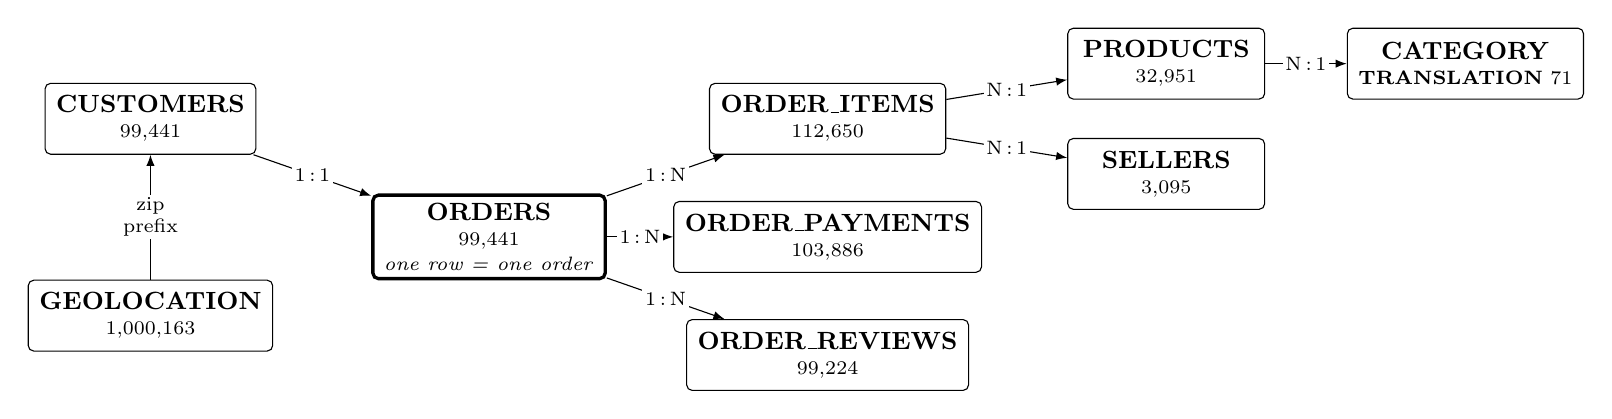
\begin{tikzpicture}[
  font=\small,
  box/.style={draw, rounded corners=2pt, minimum height=9mm, minimum width=25mm,
              inner xsep=4pt, inner ysep=3pt, align=center},
  spine/.style={box, very thick},
  link/.style={draw, -{Latex[length=4pt]}, thin},
  lbl/.style={font=\scriptsize, midway, fill=white, inner sep=1pt}
]
\node[spine] (ord) at (0,0) {\textbf{ORDERS}\\[-2pt]\scriptsize 99{,}441\\[-2pt]\scriptsize \textit{one row = one order}};

\node[box] (cus) at (-4.3,1.5) {\textbf{CUSTOMERS}\\[-2pt]\scriptsize 99{,}441};
\node[box] (itm) at (4.3,1.5) {\textbf{ORDER\_ITEMS}\\[-2pt]\scriptsize 112{,}650};
\node[box] (pay) at (4.3,0) {\textbf{ORDER\_PAYMENTS}\\[-2pt]\scriptsize 103{,}886};
\node[box] (rev) at (4.3,-1.5) {\textbf{ORDER\_REVIEWS}\\[-2pt]\scriptsize 99{,}224};

\node[box] (prd) at (8.6,2.2) {\textbf{PRODUCTS}\\[-2pt]\scriptsize 32{,}951};
\node[box] (sel) at (8.6,0.8) {\textbf{SELLERS}\\[-2pt]\scriptsize 3{,}095};
\node[box] (cat) at (12.4,2.2) {\textbf{CATEGORY}\\[-2pt]\scriptsize \textbf{TRANSLATION} 71};
\node[box] (geo) at (-4.3,-1.0) {\textbf{GEOLOCATION}\\[-2pt]\scriptsize 1{,}000{,}163};

\draw[link] (cus) -- node[lbl]{1\,:\,1} (ord);
\draw[link] (ord) -- node[lbl]{1\,:\,N} (itm);
\draw[link] (ord) -- node[lbl]{1\,:\,N} (pay);
\draw[link] (ord) -- node[lbl]{1\,:\,N} (rev);
\draw[link] (itm) -- node[lbl]{N\,:\,1} (prd);
\draw[link] (itm) -- node[lbl]{N\,:\,1} (sel);
\draw[link] (prd) -- node[lbl]{N\,:\,1} (cat);
\draw[link] (geo) -- node[lbl,align=center]{zip\\prefix} (cus);
\end{tikzpicture}}
\caption{The nine source tables. \code{ORDERS} is the analysis grain. The three
one-to-many children (items, payments and reviews) are each aggregated to one
row per order \emph{before} joining; merging them directly inflates the table by
19\% and biases every average.}
\label{fig:datamodel}
\end{figure}

\begin{table}[htbp]
\centering
\caption{Data quality audit and cleaning decisions, implemented as
\code{CLEANING\_DECISIONS} in \code{src/data\_load.py}.}
\label{tab:quality}
\small
\begin{tabular}{@{}p{2.7cm}p{4.7cm}p{6.3cm}@{}}
\toprule
\textbf{Issue} & \textbf{Evidence} & \textbf{Decision} \\
\midrule
One-to-many joins &
112{,}650 items and 103{,}886 payments against 99{,}441 orders; a naive merge
yields 118{,}437 rows &
Aggregate each child table to one row per order, then join; assert the grain \\[3pt]
Customer key &
99{,}441 \code{customer\_id} values but 96{,}096 \code{customer\_unique\_id};
2{,}997 people ordered more than once &
Carry \code{customer\_unique\_id} and group on it for repeat behaviour and for
splitting \\[3pt]
Undelivered orders &
2.98\% of orders have no delivery timestamp; status is \emph{delivered} for
97.0\% &
Delivery targets computed only for delivered orders; the rest are \code{NaN},
never imputed \\[3pt]
Review keys &
\code{review\_id} is not unique (789 ids reused); 547 orders carry 2--3 reviews
and 768 carry none &
Key on \code{order\_id}, keep the earliest review; no review means \code{NaN} \\[3pt]
Sparse review text &
\code{review\_comment\_title} present for 11.7\% of reviews,
\code{review\_comment\_message} for 41.3\% &
Use \code{review\_score} only; coverage does not support NLP features \\[3pt]
Geolocation grain &
1{,}000{,}163 rows for 19{,}010 zip prefixes, including points outside Brazil &
Collapse to a median coordinate per prefix; use it for great-circle distance \\[3pt]
Missing product attributes &
610 products (1.9\%) have no category &
Label \code{unknown} rather than dropping orders; impute numerics in-pipeline \\[3pt]
Coverage ramp &
326 orders before 2017; final weeks truncated mid-cycle &
Restrict to 2017-01-01 .. 2018-08-31 (99{,}091 orders) \\[3pt]
Portuguese categories &
71 category names &
Translate to English for all output; keep the original key \\
\bottomrule
\end{tabular}
\end{table}

\begin{table}[htbp]
\centering
\caption{Candidate problems against the brief's scoping checklist
(Section~\ref{sec:candidates}), as scored in Phase 1 with untuned probes.}
\label{tab:checklist}
\small
\begin{tabular}{@{}p{2.5cm}p{4.1cm}p{3.6cm}p{3.5cm}@{}}
\toprule
\textbf{Criterion} & \textbf{C1 delivery (checkout)} & \textbf{C2 low review (delivery)} & \textbf{C3 repeat (checkout)} \\
\midrule
Derivable target & Yes, from order timestamps & Yes, \code{review\_score} $\le 2$ & Yes, next order by person \\
No leakage & Yes, checkout regime & Yes, at-delivery regime & Yes, checkout regime \\
Sufficient signal & Regression yes ($-41\%$ MAE); classification weak (1.6$\times$) & Yes, PR-AUC 0.40 vs 0.11 (3.6$\times$) & No, 2.0$\times$ at a 1.7\% base rate \\
Manageable imbalance & 8.1\% late; PR-AUC and thresholds, no resampling & 14.6\% low; same handling & 2.6\%, too extreme \\
Clear stakeholder & Operations & Customer experience & CRM \\
\midrule
\textbf{Verdict} & \textbf{Problem 1} & \textbf{Problem 2} & Rejected \\
\bottomrule
\end{tabular}
\end{table}

\begin{table}[htbp]
\centering
\caption{Data dictionary for the nine source tables. \emph{Null} is measured,
not declared: Y means the column actually contains missing values in this
extract, with the observed rate given.}
\label{tab:dictionary}
\scriptsize
\setlength{\tabcolsep}{3.5pt}
\renewcommand{\code}[1]{\texttt{#1}}
\begin{tabular}{@{}p{2.0cm}p{4.4cm}p{1.1cm}p{1.05cm}p{5.5cm}@{}}
\toprule
\textbf{Table} & \textbf{Column} & \textbf{Type} & \textbf{Null} & \textbf{Comment} \\
\midrule
\code{orders} & \code{order\_id} & text & N & Primary key. The analysis grain \\
 & \code{customer\_id} & text & N & \textbf{Per-order} key, not a person \\
 & \code{order\_status} & text & N & 8 values; \emph{delivered} for 97.0\% \\
 & \code{order\_purchase\_timestamp} & datetime & N & The checkout prediction moment \\
 & \code{order\_approved\_at} & datetime & Y 0.16\% & Post-checkout; excluded as a feature \\
 & \code{order\_delivered\_carrier\_date} & datetime & Y 1.79\% & Post-outcome; splits lead time into seller and carrier share \\
 & \code{order\_delivered\_customer\_date} & datetime & Y 2.98\% & Post-outcome; defines both delivery targets \\
 & \code{order\_estimated\_delivery\_date} & date & N & Promised at checkout; \textbf{admissible}. Date only, 459 distinct values \\
\midrule
\code{order\_items} & \code{order\_id} & text & N & \textbf{1:N} --- 112,650 rows for 98,666 orders \\
 & \code{order\_item\_id} & int & N & Sequence within the order, 1--21 \\
 & \code{product\_id}, \code{seller\_id} & text & N & Foreign keys \\
 & \code{shipping\_limit\_date} & datetime & N & Post-checkout; excluded \\
 & \code{price}, \code{freight\_value} & float & N & Per item; summed to order level \\
\midrule
\code{order\_payments} & \code{order\_id} & text & N & \textbf{1:N}. One order has no payment row \\
 & \code{payment\_sequential} & int & N & 1--29 \\
 & \code{payment\_type} & text & N & 5 values; credit card 75.4\% \\
 & \code{payment\_installments} & int & N & 0--24; $>1$ for 51.4\% of orders \\
 & \code{payment\_value} & float & N & Summed to order level \\
\midrule
\code{order\_reviews} & \code{review\_id} & text & N & \textbf{Not unique} --- 789 ids reused across orders \\
 & \code{order\_id} & text & N & \textbf{1:N}; 547 orders carry 2--3 reviews \\
 & \code{review\_score} & int & N & 1--5; target of Problem 2 \\
 & \code{review\_comment\_title} & text & Y 88.3\% & Too sparse to use \\
 & \code{review\_comment\_message} & text & Y 58.7\% & Too sparse to use; no NLP features \\
 & \code{review\_creation\_date} & date & N & Post-outcome for the review target \\
 & \code{review\_answer\_timestamp} & datetime & N & Post-outcome \\
\midrule
\code{customers} & \code{customer\_id} & text & N & Joins 1:1 to orders \\
 & \code{customer\_unique\_id} & text & N & \textbf{The actual person}; 96,096 of them. Grouping key for splits \\
 & \code{customer\_zip\_code\_prefix} & int & N & Joins to geolocation \\
 & \code{customer\_city}, \code{customer\_state} & text & N & 4,119 cities, 27 states \\
\midrule
\code{sellers} & \code{seller\_id} & text & N & 3,095 sellers \\
 & \code{seller\_zip\_code\_prefix} & int & N & Joins to geolocation \\
 & \code{seller\_city}, \code{seller\_state} & text & N & 59.7\% of sellers are in SP \\
\midrule
\code{products} & \code{product\_id} & text & N & 32,951 products \\
 & \code{product\_category\_name} & text & Y 1.85\% & Portuguese; 73 values. Nulls labelled \emph{unknown} \\
 & \code{product\_weight\_g} & float & Y 0.01\% & Summed to order level \\
 & \code{product\_length/height/width\_cm} & float & Y 0.01\% & Combined into item volume \\
 & \code{product\_photos\_qty} & float & Y 1.85\% & Listing-quality proxy \\
\midrule
\code{geolocation} & \code{geolocation\_zip\_code\_prefix} & int & N & 19,015 prefixes over 1,000,163 rows \\
 & \code{geolocation\_lat}, \code{\_lng} & float & N & Collapsed to a median per prefix; out-of-Brazil points dropped \\
\midrule
\code{category\_} & \code{product\_category\_name} & text & N & Join key \\
\code{translation} & \code{product\_category\_name\_english} & text & N & 71 translations \\
\midrule
\multicolumn{5}{@{}l@{}}{\textit{Derived in \code{src/} --- not present in any source file:}} \\
derived & \code{delivery\_days} & float & Y & Purchase to arrival; target of 1A \\
derived & \code{is\_late} & bool & Y & Arrival after the promised date; target of 1B \\
derived & \code{distance\_km} & float & Y 1.2\% & Great-circle customer--seller distance \\
derived & \code{estimated\_days} & float & N & Promised window in days \\
derived & \code{lead\_category} & text & N & Category of the most expensive item \\
derived & \code{freight\_ratio} & float & Y & Freight as a share of item value \\
derived & \code{hist\_*} & float & Y & The eight as-of track records of Section~\ref{sec:history} \\
\bottomrule
\end{tabular}
\end{table}

\clearpage
\section{Success criteria registered in advance}
\label{app:bands}

Written into \code{config.EXPECTED\_BANDS} before any model was tuned.
\code{evaluate.check\_bands()} compares the headline results against them at the
end of every training run and writes its verdicts to
\code{report/results/bands.csv}. The alarm is direction-aware: for an error
metric the suspicious end of the interval is the low one, for a score the high
one, and confusing the two would point the check at the shortfalls and wave the
leaks through.

\begin{center}
\small
\begin{tabular}{@{}llp{2.4cm}p{5.0cm}r@{}}
\toprule
\textbf{Problem} & \textbf{Metric} & \textbf{Registered band} & \textbf{Where the range came from} & \textbf{Result} \\
\midrule
1A & MAE (days) & 3.3 -- 4.3 & Phase 1 reported 3.89 untuned & 3.898 \\
1B & balanced accuracy & 0.58 -- 0.72 & Phase 1 reported 0.58 for a direct classifier & 0.705 \\
1B & ROC-AUC & 0.72 -- 0.85 & Untuned scoping probe reached 0.79 for the derived route & 0.782 \\
2 & balanced accuracy & 0.63 -- 0.74 & Phase 1 reported 0.69 & 0.681 \\
2 & ROC-AUC & 0.70 -- 0.79 & Phase 1 reported 0.73 & 0.749 \\
2 & PR-AUC & 0.34 -- 0.48 & Phase 1 reported 0.40 against a 0.11 floor & 0.414 \\
\bottomrule
\end{tabular}
\end{center}

\section{Hyperparameter search spaces and selected values}
\label{app:hyperparameters}

\begin{center}
\scriptsize
\begin{tabular}{@{}llll@{}}
\toprule
\textbf{Family} & \textbf{Rung} & \textbf{Classification} & \textbf{Regression} \\
\midrule
A --- Linear     & 0 & \code{LogisticRegression} & \code{LinearRegression} \\
                 & 1 & \code{LogisticRegression} ($\ell_2$, tuned $C$) & \code{Ridge} (tuned $\alpha$) \\
B --- Tree-based & 0 & \code{DecisionTreeClassifier} & \code{DecisionTreeRegressor} \\
                 & 1 & \code{RandomForestClassifier} & \code{RandomForestRegressor} \\
                 & 2 & \code{HistGradientBoostingClassifier} & \code{HistGradientBoostingRegressor} \\
C --- Ensemble   & 0 & \code{VotingClassifier} (soft, A+B) & \code{VotingRegressor} (A+B) \\
                 & 1 & \code{StackingClassifier} (A+B) & \code{StackingRegressor} (A+B) \\
\bottomrule
\end{tabular}
\end{center}

Every tuned model was searched with \code{RandomizedSearchCV} over the
distributions of Table~\ref{tab:spaces}, scored by five-fold expanding-window
cross-validation inside the training period: thirty draws per model, except the
random forests, which get six because a forest costs one to two orders of
magnitude more per fit and Phase 1 had already shown the forest and the boosted
trees landing within 0.01 days of each other. Table~\ref{tab:selected} lists the
values that won, which the Phase 2 report referred to but did not print; the
deployed ensembles carry exactly their winning members' values, read back from
the pickles, and the validation suite asserts it.

\begin{table}[htbp]
\centering
\caption{Search spaces.}
\label{tab:spaces}
\small
\begin{tabular}{@{}p{4.1cm}cp{7.9cm}@{}}
\toprule
\textbf{Model} & \textbf{Draws} & \textbf{Distributions} \\
\midrule
\code{LinearRegression} / \code{LogisticRegression} & --- &
No free parameters. Fitted and scored under the same protocol so the row is
comparable \\[3pt]
\code{Ridge} & 30 & $\alpha \sim \mathrm{loguniform}(10^{-3}, 10^{3})$ \\[3pt]
\code{LogisticRegression} ($\ell_2$) & 30 & $C \sim \mathrm{loguniform}(10^{-3}, 10^{2})$ \\[3pt]
\code{DecisionTree} & 30 & \code{max\_depth} $\sim$ randint(3, 20) [classifier: (3, 16)];
\code{min\_samples\_leaf} $\sim$ randint(5, 200) [classifier: (20, 400)];
\code{max\_features} $\sim U(0.4, 1.0)$ \\[3pt]
\code{RandomForest} & 6 & 150 trees; \code{max\_depth} $\sim$ randint(8, 18)
[classifier: (6, 16)]; \code{min\_samples\_leaf} $\sim$ randint(20, 140)
[classifier: (30, 180)]; \code{max\_features} $\sim U(0.15, 0.40)$ \\[3pt]
\code{HistGradientBoosting} & 30 & \code{max\_iter} $\sim$ randint(120, 500);
\code{learning\_rate} $\sim \mathrm{loguniform}(0.02, 0.3)$;
\code{max\_leaf\_nodes} $\sim$ randint(15, 64);
\code{min\_samples\_leaf} $\sim$ randint(10, 120);
\code{l2\_regularization} $\sim \mathrm{loguniform}(10^{-4}, 10)$ \\[3pt]
\code{Voting} & --- & Weights fixed at 1:2 in the tree's favour. A stated prior,
not a tuned parameter: under drift the linear member is materially weaker and an
equal blend would be worse than its better half \\[3pt]
\code{Stacking} & --- & Meta-learner \code{Ridge}($\alpha=1$) /
\code{LogisticRegression}($C=1$); inner CV five contiguous folds --- see the note below \\
\bottomrule
\end{tabular}
\end{table}

\begin{table}[htbp]
\centering
\caption{Selected hyperparameter values, from
\code{report/results/hyperparameters.csv}. Members of the deployed ensembles are
the rows marked $\dagger$; the stacked review model's meta-learner has
coefficients 0.405 (linear member) and 5.572 (tree member).}
\label{tab:selected}
\footnotesize
\setlength{\tabcolsep}{4pt}
\begin{tabular}{@{}llp{9.6cm}@{}}
\toprule
\textbf{Problem} & \textbf{Model} & \textbf{Selected values} \\
\midrule
1A & LinearRegression $\dagger$ & no free parameters \\
1A & Ridge & $\alpha = 659.9$ \\
1A & DecisionTree & depth 17, min leaf 158, max features 0.897 \\
1A & RandomForest & 150 trees, depth 14, min leaf 107, max features 0.165 \\
1A & HistGradientBoosting $\dagger$ & 433 iterations, learning rate 0.1065, 36 leaf nodes, min leaf 117, $\ell_2$ 9.142 \\
1A & VotingRegressor $\dagger$ & weights 1:2 (linear : tree) \\
\midrule
1B & LogisticRegression ($\ell_2$) & $C = 0.004983$ \\
1B & DecisionTree & depth 9, min leaf 290, max features 0.878 \\
1B & RandomForest & 150 trees, depth 13, min leaf 132, max features 0.300 \\
1B & HistGradientBoosting & 426 iterations, learning rate 0.07079, 21 leaf nodes, min leaf 30, $\ell_2$ 8.244 \\
1B & derived route $\dagger$ & one-parameter logistic on the margin, fitted on validation; threshold 0.11 \\
\midrule
2 & LogisticRegression ($\ell_2$) $\dagger$ & $C = 8.431$ \\
2 & DecisionTree & depth 14, min leaf 211, max features 0.963 \\
2 & RandomForest & 150 trees, depth 12, min leaf 44, max features 0.349 \\
2 & HistGradientBoosting $\dagger$ & 208 iterations, learning rate 0.02073, 28 leaf nodes, min leaf 18, $\ell_2$ 0.01789 \\
2 & StackingClassifier $\dagger$ & meta-learner LogisticRegression($C = 1$); threshold 0.19 \\
\bottomrule
\end{tabular}
\end{table}

\paragraph{A compromise inside stacking, stated plainly.}
\code{StackingClassifier} and \code{StackingRegressor} build their meta-features
with \code{cross\_val\_\allowbreak predict}, which requires the inner folds to \emph{partition}
the training set: every row must be predicted exactly once. An expanding window
partitions nothing --- the earliest rows are never in a test fold --- so the
closest valid approximation is unshuffled \code{KFold}, which at least keeps each
fold contiguous in time. The meta-learner is consequently fitted on out-of-fold
predictions partly made by models trained on later orders. The residual optimism
is confined to the meta-learner's coefficients; the base models are refitted on
the whole training period afterwards, and the outer protocol scoring the
finished ensemble is still the expanding window. It matters less than it
otherwise would because of how the result lands: the ensemble is
\emph{flattered} by this arrangement and still does not separate from the
boosted trees, which makes the conclusion in
Section~\ref{sec:results-ensemble} safer rather than weaker.

\section{Re-checking a Phase 1 claim about least squares}
\label{app:encoding}

Phase 1 reported that ordinary least squares was unusable on this design matrix
--- ``rank-deficient, so its coefficients explode''. Phase 2 re-ran it four ways.
The observation reproduces exactly; the conclusion drawn from it needed
correcting.

\begin{table}[htbp]
\centering
\caption{Reproducible via \code{report/results/encoding\_diagnostic.csv}. The
deficiency is exactly four --- one per categorical, because each one-hot block
sums to one and is therefore collinear with the intercept.}
\label{tab:encoding}
\small
\begin{tabular}{@{}lccrrr@{}}
\toprule
\textbf{Encoding} & \textbf{rank / cols} & \textbf{deficiency} &
\textbf{max $|\beta|$} & \textbf{CV MAE} & \textbf{test MAE} \\
\midrule
OLS, full one-hot block   & 101 / 105 & 4 & $2.7\times10^{13}$ & $3.9\times10^{11}$ & 4.181 \\
OLS, one level dropped    & 101 / 101 & 0 & 14.7  & 5.242 & 4.181 \\
Ridge, full one-hot block & 101 / 105 & 4 & 9.82  & 5.241 & 4.182 \\
Ridge, one level dropped  & 101 / 101 & 0 & 12.5  & 5.240 & 4.183 \\
\bottomrule
\end{tabular}
\end{table}

Least squares still returns a minimum-norm solution and its \emph{predictions}
are fine --- 4.181 days on the test window, indistinguishable from Ridge. What is
not fine is the coefficient vector at $10^{13}$, and the cancellation holding it
together is fragile enough to fail on one of five expanding-window folds, which
is why the cross-validated error is astronomical while the single-split test
error looks healthy. Dropping one level per categorical restores full rank, so
the linear family is encoded that way; the compromise is that a level unseen in
training is scored as the reference level, which affects a handful of test
orders with a payment type absent from training. Once the design is full rank,
Ridge and OLS agree to three decimals: regularisation buys numerical stability
here, not accuracy.

\section{Full result tables}
\label{app:tables}

The body reports the models that matter. The complete tables --- every model,
every metric, cross-validated, validation and test scores side by side --- are
written to \code{report/results/}:

\begin{center}
\footnotesize
\begin{tabular}{@{}p{5.2cm}p{9.6cm}@{}}
\toprule
\textbf{File} & \textbf{Contents} \\
\midrule
\code{reg\_p1a.csv} & Problem 1A: baselines, both ladders, ensembles; MAE, RMSE, $R^2$ \\
\code{clf\_p1b.csv} & Problem 1B: five direct classifiers and two derived routes \\
\code{clf\_p2.csv} & Problem 2: both ladders and both ensembles, all metrics \\
\code{selection\_*.csv}, \code{cv\_folds.csv} & Every candidate on every out-of-sample window, its ranks, and the fold-to-fold spread (Appendix~\ref{app:protocol}) \\
\code{hyperparameters.csv} & Selected values of every searched model and of the deployed ensembles' members (Appendix~\ref{app:hyperparameters}) \\
\code{encoding\_diagnostic.csv} & The Phase 1 re-check of Table~\ref{tab:encoding} \\
\code{cv\_protocol.csv} & Temporal against shuffled CV against the forward test \\
\code{weight\_ablation.csv} & Class weighting: discrimination and calibration \\
\code{calibration\_p2.csv}, \code{threshold\_sweep\_p2.csv} & Reliability and the operating-point sweep \\
\code{cost\_p2.csv}, \code{cost\_p1b.csv} & Expected net benefit by threshold \\
\code{perm\_p1a.csv}, \code{perm\_p2.csv} & Permutation importance on the test window \\
\code{segments\_*.csv} & Performance by region, category and test month \\
\code{predictions\_*.csv} & Per-order test predictions, from which the figures and the application's replay are drawn \\
\code{bands.csv} & Headline metrics against the bands registered in advance \\
\code{capacity\_*.csv} & Precision@$K$ and Recall@$K$, pooled and per day, for both flags \\
\code{lateness\_*.csv} & The lateness anatomy of Appendix~\ref{app:lateness} \\
\code{train\_val\_test.csv} & The deployed models on the training, validation and test periods (Appendix~\ref{app:tvt}) \\
\code{pilot\_design.csv}, \code{pilot\_breakeven.csv} & The outreach pilot sizing (Appendix~\ref{app:pilot}) \\
\code{review\_timing*.csv}, \code{story\_order.csv} & Review timing against delivery, the reachable share of the call list, the restated value, the on-time check and the example order (Appendix~\ref{app:timing}) \\
\bottomrule
\end{tabular}
\end{center}

\section{The cross-validation protocol, and every candidate on every window}
\label{app:protocol}

\begin{table}[htbp]
\centering
\caption{One model, three protocols. Raw average precision disagrees; the same
numbers divided by each period's no-skill floor do not.
Figure~\ref{fig:protocol}.}
\label{tab:protocol}
\small
\begin{tabular}{@{}lrrrr@{}}
\toprule
\textbf{Protocol} & \textbf{PR-AUC} & \textbf{fold spread} & \textbf{no-skill floor} & \textbf{lift} \\
\midrule
\code{TimeSeriesSplit}, expanding window & 0.562 & $\pm$0.091 & 0.158 & 3.55$\times$ \\
\code{StratifiedGroupKFold}, shuffled    & 0.580 & $\pm$0.006 & 0.158 & 3.66$\times$ \\
Forward test window --- the truth        & 0.414 & ---        & 0.110 & 3.75$\times$ \\
\bottomrule
\end{tabular}
\end{table}

Both cross-validated estimates in Table~\ref{tab:protocol} sit about 0.16 above
the forward result, which looks like catastrophic optimism --- and almost all
of it is mechanical. Average
precision's no-skill baseline \emph{is} the positive rate
\citep{saito2015prplot}, and the low-review rate falls from 15.8\% inside the
training period to 11.0\% in the test window; normalised by that floor the three
agree to within 0.2 of a multiple. \textbf{Raw PR-AUC is not comparable across
periods with different base rates; its lift over the floor is} --- and quoting
the raw number alone would have supported either a claim of severe overfitting or
a claim of none. The shuffled protocol adds a second warning: its fold-to-fold
spread is $\pm$0.006 against the temporal protocol's $\pm$0.091, an interval
fifteen times narrower on an estimate no closer to the truth.

\begin{table}[htbp]
\centering
\caption{Every Problem 2 candidate on every out-of-sample window (PR-AUC), from
\code{report/results/cv\_folds.csv}; the standard deviation is over the five
expanding folds. ``Rank'' is the mean rank over the three most recent windows
(folds 4, 5 and validation), the selection criterion of
Section~\ref{sec:cv}. Figure~\ref{fig:cvfolds}. The same table for Problems 1A
and 1B is in the CSV.}
\label{tab:cvfolds}
\scriptsize
\setlength{\tabcolsep}{2.6pt}
\resizebox{\linewidth}{!}{%
\begin{tabular}{@{}lrrrrrrrrrr@{}}
\toprule
\textbf{Model} & \textbf{fold 1} & \textbf{fold 2} & \textbf{fold 3} & \textbf{fold 4} & \textbf{fold 5} & \textbf{val.} & \textbf{mean $\pm$ sd} & \textbf{test} & \textbf{rank} \\
\midrule
StackingClassifier (A+B) \emph{deployed} & 0.413 & 0.537 & 0.617 & 0.660 & 0.614 & 0.409 & 0.568 $\pm$ 0.087 & 0.414 & 1.67 \\
HistGradientBoosting   & 0.411 & 0.539 & 0.618 & 0.660 & 0.613 & 0.407 & 0.568 $\pm$ 0.088 & 0.415 & 2.00 \\
RandomForest           & 0.404 & 0.544 & 0.622 & 0.654 & 0.616 & 0.403 & 0.568 $\pm$ 0.089 & 0.405 & 2.67 \\
VotingClassifier (A+B) & 0.413 & 0.526 & 0.611 & 0.650 & 0.604 & 0.404 & 0.561 $\pm$ 0.084 & 0.407 & 3.67 \\
DecisionTree           & 0.380 & 0.510 & 0.595 & 0.640 & 0.592 & 0.389 & 0.543 $\pm$ 0.092 & 0.396 & 5.00 \\
LogisticRegression ($\ell_2$) & 0.306 & 0.416 & 0.534 & 0.574 & 0.497 & 0.320 & 0.466 $\pm$ 0.095 & 0.291 & 6.33 \\
LogisticRegression     & 0.307 & 0.416 & 0.534 & 0.574 & 0.497 & 0.320 & 0.465 $\pm$ 0.095 & 0.291 & 6.67 \\
\bottomrule
\end{tabular}}
\end{table}

Table~\ref{tab:cvfolds} is what the Phase 2 evaluation asked for. Read down a
column, the windows differ far more than the models: every candidate is at its
worst on the first fold (early 2017, few orders, a 20\% low-review rate) and at
its best on the fourth. Read across a row, the three tree-based rungs are within
0.0004 of one another on the cross-validated mean against a fold-to-fold
standard deviation of 0.09; the stacked ensemble is ahead of the single boosted
model on three of the six windows and behind on three. Cross-validation cannot
order them, which is why the rank rule was fixed before any test score was seen
and why the deployed choice is reported as a tie resolved by that rule rather
than as a win.

\section{Lateness anatomy: where the late deliveries came from}
\label{app:lateness}

Phase 1 read the monthly late-rate series and attributed its spikes to Black
Friday and to the May 2018 truckers' strike. The Phase 1 feedback pointed out
that the figure does not support the second claim --- the largest peaks are
February and March 2018, and May is unremarkable --- and asked for a source and
a more careful link. \code{src/lateness\_anatomy.py} is that analysis, at three
resolutions, and Figure~\ref{fig:lateness} draws it.

\paragraph{Weekly, not monthly.} A ten-day event cannot be resolved by a
monthly series. In Monday-to-Sunday purchase weeks the strike of 21 May to
1 June 2018 \citep{bloomberg2018strike} --- nationwide road blockades, during
which Correios suspended its time-definite Sedex services and added five
business days to standard parcels \citep{tecnoblog2018correios} --- is plainly
visible, but one week \emph{earlier} than a naive reading expects: orders placed
on 14--20 May were promised 19.5 days under normal conditions and were in
transit when the roads closed, and 16.0\% of them arrived late against a 5.0\%
average over the preceding five weeks. Of all orders in transit during the
strike (4{,}228), 16.9\% were late, against 0.4\% for the May orders delivered
before it (Table~\ref{tab:strike}). What the monthly series records instead is
the platform's reaction: order volume in the strike week halved, the promised
window for orders placed that week rose to 25.3 days and in the following week
to 36.8, and the late rate of those orders was 5.5\% and 0.4\%. That is why June
2018, at 1.4\%, is the quietest month in the data.

\paragraph{February--March 2018 is a different mechanism.} Panel (b) of
Figure~\ref{fig:lateness} splits lead time at the carrier handoff. Outside the
peak, sellers hand parcels to the carrier in about 3.2 days and the carrier
takes 8.7 more; in February--March 2018 the seller's share was unchanged at
3.4 days while the carrier's rose to 13.2, in every customer region. At the
same time the promised window was \emph{tightened}, from 26.3 days in January
to 22.0 in March --- within the S\~{a}o Paulo to S\~{a}o Paulo route alone, from
20.1 to 15.2 days --- so the slack that normally absorbs a slow fortnight was
removed exactly when it was needed. The late rate peaked at 29.0\% in the week
of 26 February, the promise was lengthened again from the week of 9 April, and
by that week the late rate was back under 5\%. The data do not identify the
external cause of the carrier slowdown and we do not assert one; what they do
establish is that it was carrier-side, network-wide and compounded by a
promising decision, which is the careful form of the claim Phase 1 made loosely.

\begin{table}[htbp]
\centering
\caption{The cohorts around the strike, from
\code{report/results/lateness\_strike.csv}. Carrier days run from the carrier
handoff to the doorstep; the promise is the window quoted at checkout.}
\label{tab:strike}
\footnotesize
\begin{tabular}{@{}lrrrr@{}}
\toprule
\textbf{Cohort} & \textbf{orders} & \textbf{late} & \textbf{carrier days} & \textbf{promise, days} \\
\midrule
Bought 1--20 May, delivered before the strike & 2{,}749 & 0.4\%  & 4.8  & 19.5 \\
In transit during the strike                  & 4{,}228 & 16.9\% & 13.1 & 25.5 \\
Bought during the strike, 21 May--1 June      & 1{,}502 & 3.5\%  & 9.2  & 29.4 \\
Bought 2--30 June                             & 5{,}912 & 1.4\%  & 6.7  & 27.5 \\
\bottomrule
\end{tabular}
\end{table}

\clearpage
\section{Responses to the Phase 1 and Phase 2 feedback}
\label{app:feedback}

Both rounds of evaluator feedback were treated as specifications.
Tables~\ref{tab:feedback1} and \ref{tab:feedback2} list each point and the
section, table or figure of this report that acts on it.

\begin{center}
\begin{minipage}{\linewidth}
\centering
\captionof{table}{Phase 1 feedback (on the literature review, the exploratory
analysis and the dashboard) and where this report acts on it.}
\label{tab:feedback1}
\small
\begin{tabular}{@{}p{4.4cm}p{10.1cm}@{}}
\toprule
\textbf{Feedback} & \textbf{Response} \\
\midrule
Survey-based perceived quality and platform ratings were treated as one construct &
Sections~\ref{sec:lit} and \ref{sec:problem} separate them, cite the
self-selection literature \citep{hu2009jshaped, hu2017selfselection,
dellarocas2003digitization}, and define the target as the platform rating;
Section~\ref{sec:limitations} carries the consequence \\[2pt]
Model choices cited original algorithm papers rather than e-commerce
applications; no comparison within the tree family; HistGradientBoosting not
justified &
Section~\ref{sec:lit} argues the rungs from the empirical comparisons and from
e-commerce applications, including three studies on this dataset, and states
why HistGradientBoosting; the ladder results of Section~\ref{sec:results} are
the within-family comparison \\[2pt]
Features not supported by literature &
Section~\ref{sec:features} cites the support for each feature group and uses
the correlation matrix as the empirical screen; Appendix~\ref{app:features}
gives a rationale per feature \\[2pt]
Problem 2 should be evaluated under limited capacity, with Precision@$K$ and
Recall@$K$ &
Section~\ref{sec:results-capacity}, Table~\ref{tab:capacity} and
Figure~\ref{fig:capacity}; the operating point in Section~\ref{sec:cost} is a
capacity; the application returns a top-$K$ triage list and replays any test
day \\[2pt]
Figure 3 attributed the late-rate peaks to the May 2018 strike; the strike
needed a source &
Section~\ref{sec:eda-lateness}, Appendix~\ref{app:lateness} and
Figure~\ref{fig:lateness}: the peaks are February--March 2018; the strike is
cited \citep{bloomberg2018strike, tecnoblog2018correios}, shown at weekly
resolution, and its effect traced through the promised window \\[2pt]
Figure 5a omitted S\~{a}o Paulo; ``roughly triples''; Figure 8 not referenced &
Figure~\ref{fig:geography}a redrawn (the notebook had taken the first eight
states alphabetically); growth is about eight-fold
(Section~\ref{sec:temporal}); the correlation matrix is discussed in
Sections~\ref{sec:eda} and \ref{sec:features} \\[2pt]
Candidate 1 named a stakeholder without saying how the team would use the
prediction &
Table~\ref{tab:levers} and Section~\ref{sec:stakeholders}: four levers ordered
by cost, each with its trigger and the evidence behind it \\[2pt]
Dashboard inaccessible &
Redeployed from the team's current repository under a new URL;
Section~\ref{sec:deployment} explains how it stays reachable \\
\bottomrule
\end{tabular}
\end{minipage}
\end{center}

\begin{center}
\begin{minipage}{\linewidth}
\centering
\captionof{table}{Phase 2 feedback (on the modelling report) and where this
report acts on it.}
\label{tab:feedback2}
\small
\begin{tabular}{@{}p{4.4cm}p{10.1cm}@{}}
\toprule
\textbf{Feedback} & \textbf{Response} \\
\midrule
Report CV scores with their fold-to-fold variation for the Problem 2
candidates &
Table~\ref{tab:review} now carries the mean $\pm$ standard deviation over the
five folds for every candidate (and Table~\ref{tab:reg} for the regression);
Table~\ref{tab:cvfolds} and Figure~\ref{fig:cvfolds} show every candidate on
every window; Section~\ref{sec:results-review} interprets the spread; the
model card shows the same table \\[2pt]
State the deployed Problem 2 model clearly and consistently; justify the
choice &
Section~\ref{sec:results-ensemble} and Table~\ref{tab:deployed}: the
StackingClassifier, as pickled, with the justification; the README, the model
card and this text are tied to the artifact by a validation check \\[2pt]
Refer to Figure 3 in the text; the selected hyperparameter values were said to
be in Appendix C but were not &
Every figure in Appendix~\ref{app:figures} is referred to from the body; the
selected values are in Table~\ref{tab:selected}, generated from the results
tables and the deployed pickles \\[2pt]
The expected benefit assumes that contacting a customer prevents the low
review; state it as a limitation and propose a pilot or A/B test &
Section~\ref{sec:limitations} states it; Section~\ref{sec:pilot},
Appendix~\ref{app:pilot} and Figure~\ref{fig:pilot} design and size the
randomised pilot; the model card carries a calculator for it.
Appendix~\ref{app:timing} adds the part of the assumption the data \emph{can}
check --- whether the customer has already written --- and restates the value
on the reachable share \\
\bottomrule
\end{tabular}
\end{minipage}
\end{center}

\section{Training, validation and test side by side}
\label{app:tvt}

The results tables carry cross-validated, validation and test columns. The
in-sample fit on the training period is the missing fourth view, and it is what
separates over-fitting from drift: a model that has memorised its training
period collapses between training and validation, while a model facing a
changed world drops between validation and test, or in step with the base rate.
\code{src/fit\_diagnostics.py} scores the three deployed artifacts on all three
periods without refitting anything.

\begin{table}[htbp]
\centering
\caption{The deployed models on the training, validation and test periods.
Thresholds and the margin-to-risk mapping are the ones fitted on the validation
period and shipped. Lift is PR-AUC divided by that period's own positive rate.}
\label{tab:tvt}
\footnotesize
{\setlength{\tabcolsep}{2.3pt}
\resizebox{\linewidth}{!}{%
\begin{tabular}{@{}llrrrrrrrr@{}}
\toprule
\textbf{Model} & \textbf{Period} & \textbf{$n$} & \textbf{MAE} & \textbf{RMSE} & \textbf{$R^2$} & & & & \\
\midrule
P1A lead time (Voting)      & training   & 70{,}617 & 4.718 & 7.807 & 0.408 & & & & \\
                            & validation & 12{,}957 & 4.784 & 6.592 & 0.222 & & & & \\
                            & test       & 12{,}630 & 3.898 & 5.342 & 0.009 & & & & \\
\midrule
 & & \textbf{$n$} & \textbf{positives} & \textbf{ROC-AUC} & \textbf{PR-AUC} & \textbf{lift} & \textbf{bal.\ acc} & \textbf{F1} & \textbf{Brier} \\
\midrule
P1B late flag (derived)     & training   & 70{,}617 & 8.8\%  & 0.803 & 0.396 & 4.48$\times$ & 0.713 & 0.391 & 0.068 \\
                            & validation & 12{,}957 & 5.0\%  & 0.787 & 0.166 & 3.34$\times$ & 0.648 & 0.227 & 0.044 \\
                            & test       & 12{,}630 & 7.4\%  & 0.782 & 0.214 & 2.89$\times$ & 0.705 & 0.235 & 0.066 \\
\midrule
P2 low review (Stacking)    & training   & 72{,}380 & 15.8\% & 0.836 & 0.617 & 3.90$\times$ & 0.754 & 0.601 & 0.089 \\
                            & validation & 13{,}094 & 11.4\% & 0.762 & 0.409 & 3.60$\times$ & 0.678 & 0.436 & 0.083 \\
                            & test       & 12{,}855 & 11.0\% & 0.749 & 0.414 & 3.75$\times$ & 0.681 & 0.470 & 0.078 \\
\bottomrule
\end{tabular}}}
\end{table}

Three readings. \textbf{The lead-time blend does not memorise its training
period}: its in-sample MAE, 4.72 days, is level with the validation period's
4.78 and \emph{above} the test window's 3.90, and the fall in $R^2$ from 0.41
in-sample to 0.01 on test is the test period's small variance rather than a
large error --- the level shift of Section~\ref{sec:limitations}, not
over-fitting. \textbf{The derived late flag is stable}: ROC-AUC 0.80, 0.79, 0.78
across the three periods, while its lift over the floor falls from 4.5$\times$
to 2.9$\times$ only because the floor itself moves with the late rate.
\textbf{The stacking ensemble shows the expected, modest in-sample optimism of a
tree ensemble}: ROC-AUC 0.84 on the period it was fitted to against 0.76 and
0.75 on the two it never saw, and PR-AUC 0.62 against 0.41 --- but validation
and test agree with each other (lift 3.6$\times$ and 3.75$\times$, Brier
improving from 0.089 to 0.078 as the base rate falls), which is the comparison
that governs deployment.

\section{Feature catalogue}
\label{app:features}

Every feature, with its definition, the reason it is in the model and the
moment it becomes knowable. Literature pointers are to the works discussed in
Section~\ref{sec:lit}; empirical pointers are to Section~\ref{sec:eda}. All 36
are built by \code{src/features.py} from the nine tables alone.

{\footnotesize
\renewcommand{\code}[1]{\texttt{#1}}
\setlength{\tabcolsep}{3pt}
\begin{longtable}{@{}p{3.3cm}p{3.9cm}p{6.6cm}p{1.2cm}@{}}
\caption{The 36 features by group. ``Checkout'' features are admissible for
both problems; ``delivery'' features only for Problem 2.}
\label{tab:features} \\
\toprule
\textbf{Feature} & \textbf{Definition} & \textbf{Why it is in the model} & \textbf{Known at} \\
\midrule
\endfirsthead
\toprule
\textbf{Feature} & \textbf{Definition} & \textbf{Why it is in the model} & \textbf{Known at} \\
\midrule
\endhead
\bottomrule
\endfoot
\multicolumn{4}{@{}l}{\textit{The promise (2)}} \\
\code{estimated\_days} & promised delivery date minus purchase time, days & the platform's own routing knowledge, shown to the customer at checkout; strongest single correlate of lead time after distance ($r = 0.38$) and a decision variable in its own right \citep{cui2024promise, salari2022delivery} & checkout \\
\code{long\_promise} & promised window above the pinned median of 23.2 days & flags the routes the platform itself expects to be slow; pinned so serving and training use the same cut & checkout \\
\multicolumn{4}{@{}l}{\textit{Basket and money (11)}} \\
\code{n\_items}, \code{n\_sellers} & items and distinct sellers in the order & multi-item and multi-seller orders consolidate before shipping; order composition is the standard control in order-level logistics studies \citep{deshpande2023logistics} & checkout \\
\code{is\_multi\_seller} & more than one seller & split shipments wait for the slowest seller & checkout \\
\code{log\_price} & $\log(1 + \text{item total})$ & money is right-skewed; the log stabilises the linear family; price relates to the rating, not to lead time (Figure~\ref{fig:correlations}) & checkout \\
\code{price\_per\_item} & item total divided by items & separates one expensive item from many cheap ones & checkout \\
\code{total\_freight} & freight paid, R\$ & the platform's own pricing of distance and bulk & checkout \\
\code{freight\_ratio} & freight divided by item total & the delivery cost as the customer experiences it, relative to the purchase & checkout \\
\code{log\_weight}, \code{max\_volume\_cm3} & $\log(1 + \text{total weight})$; bulkiest item's volume & handling and carrier constraints; physical attributes are standard delivery-time inputs \citep{salari2022delivery} & checkout \\
\code{total\_photos} & listing photos across the items & a listing-quality proxy for the expectation gap behind a low rating & checkout \\
\code{max\_installments} & largest instalment count & payment behaviour and an affordability signal characteristic of this market & checkout \\
\multicolumn{4}{@{}l}{\textit{Calendar (6)}} \\
\code{purchase\_month}, \code{purchase\_dow}, \code{purchase\_hour} & month, weekday, hour of purchase & seasonality and the weekly and daily rhythm of fulfilment (Figure~\ref{fig:rhythm}); the usual calendar encodings for transactional data \citep{kuhn2019feature, heaton2016feature} & checkout \\
\code{is\_weekend}, \code{is\_business\_hours} & weekend; 09:00--18:00 & an order placed outside working hours waits for the next handling day & checkout \\
\code{is\_nov\_peak} & purchased on or after 20 November & the Black Friday surge stresses fulfilment: the late rate reached 14.3\% in November 2017 (Section~\ref{sec:eda-lateness}) & checkout \\
\multicolumn{4}{@{}l}{\textit{Geography (4)}} \\
\code{log\_distance} & $\log(1 + \text{km})$ between postcode centroids & the strongest checkout-time correlate of lead time ($r = 0.39$); distance is the backbone of delivery-time models \citep{liu2021lastmile} & checkout \\
\code{same\_state} & seller and customer in the same state & the cheapest route class; only 35.7\% of orders & checkout \\
\code{customer\_state} & destination state (27 levels) & regional logistics; rare levels pooled by the encoder & checkout \\
\code{seller\_region} & origin region (5 levels) & origin logistics, collapsed from 27 states so the linear family is not swamped by sparse levels & checkout \\
\multicolumn{4}{@{}l}{\textit{Catalogue and payment (2)}} \\
\code{lead\_category} & category of the most expensive item (74 levels, rare ones pooled) & product type drives both handling and expectations; the category's effect is otherwise invisible to the model & checkout \\
\code{lead\_payment\_type} & payment method of the largest payment & a boleto is paid at a bank and clears days after a card, so handling starts later; the top permutation feature for lead time (Section~\ref{sec:insight}) & checkout \\
\multicolumn{4}{@{}l}{\textit{Track records (8), each an as-of aggregate over orders that had closed before this one was placed}} \\
\code{hist\_seller\_\allowbreak lead\_days}, \code{hist\_seller\_\allowbreak late\_rate}, \code{hist\_seller\_\allowbreak low\_review\_rate} & the seller's mean lead time, late rate and 1--2 star rate over at least five earlier orders & a party's past performance is the standard predictor in supply-chain delay models \citep{baryannis2019risk}; the time-respecting form of target encoding \citep{miccibarreca2001target} & checkout \\
\code{hist\_seller\_n} & number of earlier orders the seller estimate rests on & cold start as information: the model can discount a seller it has barely seen & checkout \\
\code{hist\_route\_\allowbreak lead\_days} & mean lead time on the seller-state to customer-state route & origin--destination history, the route-level analogue of the above \citep{salari2022delivery} & checkout \\
\code{hist\_category\_\allowbreak low\_review\_rate} & the category's past 1--2 star rate & categories differ in how often they disappoint; encoded without seeing the future & checkout \\
\code{hist\_platform\_\allowbreak lead\_days}, \code{hist\_platform\_\allowbreak late\_rate} & platform-wide trailing 28-day mean lead time and late rate & the drift tracker: tells the model how fast the network is running right now \citep{gama2014drift} & checkout \\
\multicolumn{4}{@{}l}{\textit{Delivery outcome (3), Problem 2 only}} \\
\code{delivery\_days}, \code{delay\_vs\_\allowbreak estimate\_days}, \code{is\_late} & realised lead time; days late against the promise; late flag & the dominant driver of a 1--2 star review, 9.2\% to 54.0\% (Section~\ref{sec:reviews}; \citealt{deshpande2023logistics}); known once the parcel has arrived and forbidden before & delivery \\
\end{longtable}}

\section{The outreach pilot}
\label{app:pilot}

\begin{table}[htbp]
\centering
\caption{Pilot size by assumed effect, from \code{report/results/pilot\_design.csv}.
The control-arm rate is the model's precision at that daily capacity on the
test window; $n$ is orders per arm for a two-sided two-proportion test at
$\alpha = 0.05$; duration assumes $K$ contacts a day split evenly across the
arms; net benefit per contact is under the R\$5 : R\$40 assumption.
Figure~\ref{fig:pilot}.}
\label{tab:pilot}
\scriptsize
\setlength{\tabcolsep}{3pt}
\begin{tabular}{@{}rrrrrrrr@{}}
\toprule
\textbf{$K$/day} & \textbf{control} & \textbf{reduction} & \textbf{treated} & \textbf{$n$/arm (80\%)} & \textbf{wks (80\%)} & \textbf{wks (90\%)} & \textbf{net/contact} \\
\midrule
10 & 0.572 & 15\% & 0.486 & 531 & 16 & 21 & $-$R\$1.57 \\
10 & 0.572 & 20\% & 0.457 & 299 & 9  & 12 & $-$R\$0.43 \\
10 & 0.572 & \textbf{21.9\% (break-even)} & 0.447 & 250 & 8 & --- & R\$0.00 \\
10 & 0.572 & 25\% & 0.429 & 191 & 6  & 8  & R\$0.72 \\
10 & 0.572 & 30\% & 0.400 & 133 & 4  & 6  & R\$1.86 \\
10 & 0.572 & 40\% & 0.343 & 74  & 3  & 3  & R\$4.15 \\
\midrule
20 & 0.440 & 20\% & 0.352 & 484 & 7  & 10 & $-$R\$1.48 \\
20 & 0.440 & \textbf{28.4\% (break-even)} & 0.315 & 235 & 4 & --- & R\$0.00 \\
20 & 0.440 & 30\% & 0.308 & 210 & 3  & 5  & R\$0.28 \\
20 & 0.440 & 40\% & 0.264 & 115 & 2  & 3  & R\$2.04 \\
\bottomrule
\end{tabular}
\end{table}

The design randomises inside the top-$K$ list, so both arms share the same
predicted risk and the comparison is a fair one. Two things follow from the
table that a verbal recommendation would miss. The break-even effect grows with
capacity --- 21.9\% at ten contacts a day, 28.4\% at twenty, 42.1\% at forty ---
because precision falls as the list is worked deeper, so a contact lower down
has less to prevent; a pilot should therefore run at the capacity that would
actually be deployed. And the pilot is short at the effect sizes that matter:
six weeks detects a one-in-four reduction at ten contacts a day, while an effect
too small to pay for itself would take sixteen weeks to confirm, which is itself
informative --- if the pilot has not found an effect in two months, the policy
should not be scaled.

\section{When is the review written?}
\label{app:timing}

Problem 2 is framed at delivery, before the review is written. Olist's review
table carries two timestamps --- \code{review\_creation\_date}, the day the
satisfaction survey was sent, and \code{review\_answer\_timestamp}, the moment
the customer answered --- and comparing the second with the delivery timestamp
tests that framing (\code{src/review\_timing.py}). It holds for parcels that
arrive on time and fails for most late ones. The survey goes out at delivery or,
for a parcel still on the road, once the promised date has passed, so the
customer of a late parcel is usually asked to review while still waiting
(Table~\ref{tab:timing}).

\begin{table}[htbp]
\centering
\caption{Review timing on the 95{,}561 delivered and reviewed orders of the
analysis window, from \code{report/results/review\_timing.csv}. A negative median
means the review was answered before the parcel arrived.}
\label{tab:timing}
\small
\begin{tabular}{@{}lrr@{}}
\toprule
 & \textbf{Late parcels} & \textbf{On-time parcels} \\
\midrule
Delivered and reviewed orders & 7{,}659 & 87{,}902 \\
1--2 star rate & 54.0\% & 9.2\% \\
Survey sent on or after the promised date & 99.0\% & 2.1\% \\
1--2 star reviews written before the parcel arrived & \textbf{87.3\%} & 0.5\% \\
Share of all 1--2 star reviews & 33.8\% & 66.2\% \\
Median answer of a 1--2 star review, days after delivery & $-$4.5 & 2.1 \\
\bottomrule
\end{tabular}
\end{table}

\begin{table}[htbp]
\centering
\caption{The review-risk list on the test window, its hits split into customers
who had not yet written (reachable) and those who already had, from
\code{report/results/review\_timing\_capacity.csv}. Precision is the share of
contacts that reach a 1--2 star reviewer; the two columns after it sum to it.}
\label{tab:timing-capacity}
\small
\begin{tabular}{@{}lrrrr@{}}
\toprule
\textbf{Capacity} & \textbf{precision} & \textbf{reachable} & \textbf{already written} & \textbf{late share of contacts} \\
\midrule
top 1\%  & 0.705 & 0.419 & 0.287 & 0.403 \\
top 5\%  & 0.678 & 0.362 & 0.316 & 0.521 \\
top 10\% & 0.475 & 0.302 & 0.173 & 0.376 \\
5 a day  & 0.631 & 0.353 & 0.278 & 0.434 \\
10 a day & \textbf{0.572} & \textbf{0.352} & 0.220 & 0.362 \\
20 a day & 0.440 & 0.288 & 0.152 & 0.298 \\
\midrule
contacting at random & 0.110 & 0.093 & 0.017 & --- \\
\bottomrule
\end{tabular}
\end{table}

Two consequences follow. \textbf{A hit is not always a review that can still be
prevented.} At ten contacts a day, 0.572 of contacts reach a would-be low
reviewer, but 0.220 reach one who has already written --- almost always on a late
parcel --- and 0.352 one who has not, against 0.093 at random
(Table~\ref{tab:timing-capacity}). Counting only the reachable, the expected
benefit under R\$5 : R\$40 falls from R\$1{,}466 to \textbf{R\$775 per thousand
delivered orders} at the same optimum (threshold 0.11), and at ten contacts a
day from R\$853 to R\$433. It stays positive: reachable precision is still almost
three times the 0.125 break-even. \textbf{The action for a late parcel belongs on
the promised date, not at delivery.} Customer care can reach the customer as the
promise breaks, with an apology and a new date, and the survey can be sent after
the parcel arrives. That contact needs no model, since the calendar identifies
the parcels, and it is tested as the second arm of the pilot
(Section~\ref{sec:pilot}). The review-risk list keeps its value for the parcels
that arrive on time, which produce two thirds of all low reviews and are reviewed
a median 2.1 days after delivery. On those parcels alone the deployed model
reaches ROC-AUC 0.711, and its top 5\% are 53.8\% low reviewers, 5.7 times their
base rate, so the list does more than restate lateness
(\code{review\_timing\_subsets.csv}).

The order that opens the presentation shows the pattern in one case. Bought on 16
July 2018 in São Gonçalo (RJ) from a seller in São Luís (MA), 2{,}267\,km away,
and promised in 21 days, it was surveyed two days after the promise passed and
rated one star 5.8 days before it arrived, 10.5 days late. It tops the 16 July
review-risk list at 0.85; eight of that day's top ten left a 1--2 star review,
four of them before their parcel arrived (\code{story\_order.csv}).

\section{Contributions}
\label{app:contributions}

\begin{center}
\small
\begin{tabular}{@{}lp{11.2cm}@{}}
\toprule
\textbf{Member} & \textbf{Contribution} \\
\midrule
Pan Pinyou & Problem scoping and stakeholder framing; feature engineering for the
track-record features; business interpretation, the cost analysis and the pilot
design; report Sections~\ref{sec:problem}, \ref{sec:features} and
\ref{sec:insight}; presentation slides \\[3pt]
Li Yudan & Literature review and its revision; modelling pipeline and the family
ladders; hyperparameter search; imbalance, calibration and fold-to-fold
analysis; report Sections~\ref{sec:lit}, \ref{sec:method} and
\ref{sec:results-review} \\[3pt]
Zhu Gengyu & Data pipeline and the leakage guard; exploratory analysis and the
lateness anatomy; cross-validation protocol and the direct-against-derived
comparison; dashboard, deployment, tests and reproducibility; report
Sections~\ref{sec:data}, \ref{sec:eda}, \ref{sec:results-reg},
\ref{sec:deployment} and \ref{sec:limitations} \\
\bottomrule
\end{tabular}
\end{center}

All three members reviewed every section and verified the reported numbers
against \code{report/stats\_phase3.txt} and \code{report/stats.txt}.

\clearpage
\section{Figures}
\label{app:figures}

Figures~\ref{fig:coverage} to \ref{fig:candidates} are the exploratory analysis,
drawn by notebooks 01--04; Figures~\ref{fig:ladder} to \ref{fig:pilot} are
drawn by \code{src/figures\_phase2.py} from the same CSV tables the body's
numbers come from, so a figure cannot disagree with a table;
Figures~\ref{fig:app-predict} to \ref{fig:app-card} are the deployed
application.

\begin{figure}[htbp]
  \centering
  \includegraphics[width=\linewidth]{fig01_coverage_quality.pdf}
  \caption{(a) Monthly order volume. The pilot period before 2017 contributes 326
  orders in total and is excluded from the analysis window. (b) Missingness by
  column: structural rather than random, dominated by orders that never reached
  the customer.}
  \label{fig:coverage}
\end{figure}

\begin{figure}[htbp]
  \centering
  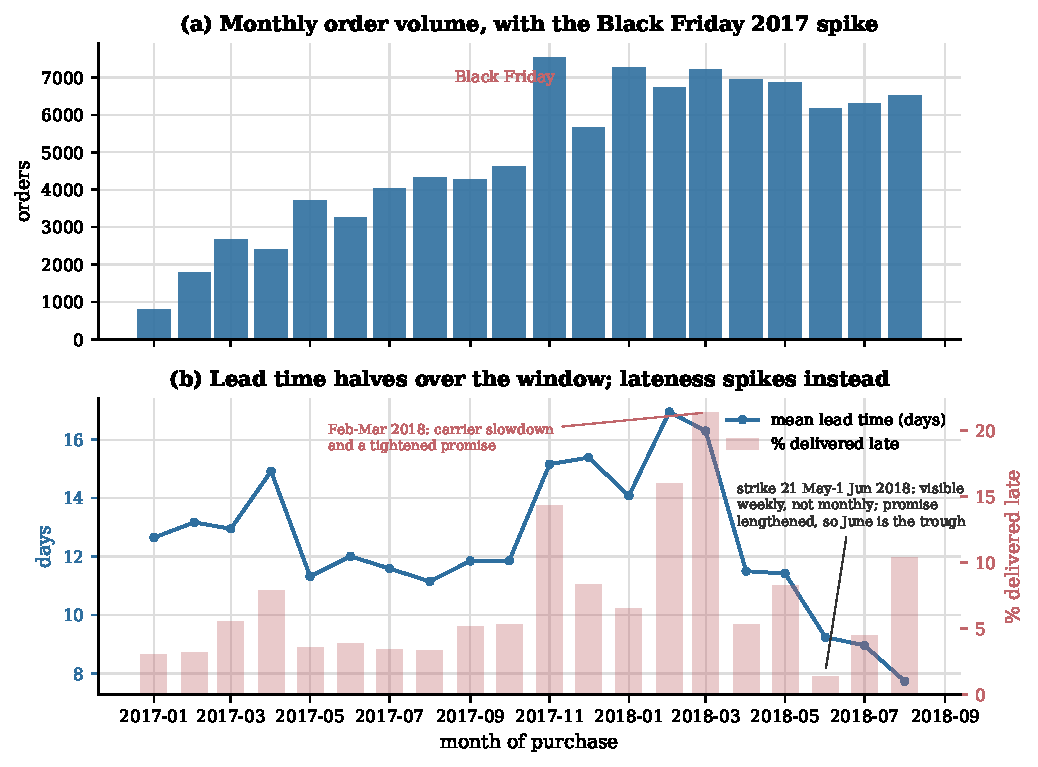
\includegraphics[width=\linewidth]{fig02_volume_drift.pdf}
  \caption{(a) Order volume with the Black Friday 2017 spike. (b) The central
  temporal finding: mean delivery lead time halves across the window (line, left
  axis) while the late rate is volatile rather than trending (bars, right axis).
  The spikes are Black Friday (November 2017) and February--March 2018, a
  carrier-side slowdown that coincided with a tightened promise. The truckers'
  strike of 21 May--1 June 2018 is not visible at monthly resolution
  (Section~\ref{sec:eda-lateness}).}
  \label{fig:volume}
\end{figure}

\begin{figure}[htbp]
  \centering
  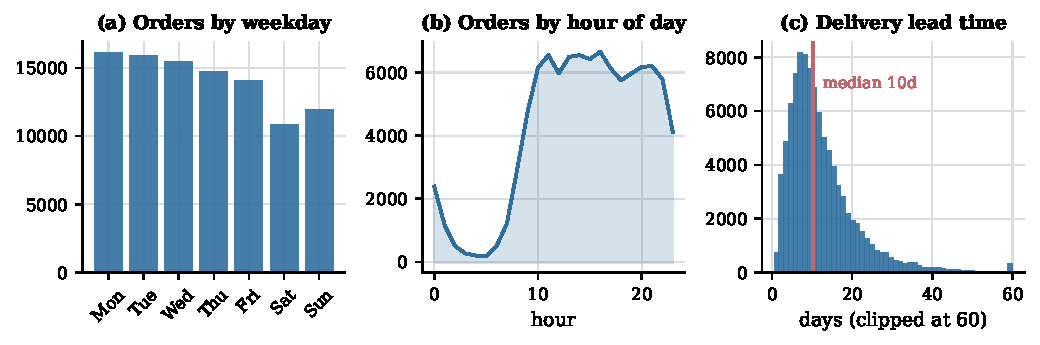
\includegraphics[width=\linewidth]{fig03_rhythm.pdf}
  \caption{Purchase rhythm and the lead-time distribution. Ordering is
  weekday-heavy and peaks at 16:00; lead time is right-skewed with a median of
  10.2 days and a long tail.}
  \label{fig:rhythm}
\end{figure}

\begin{figure}[htbp]
  \centering
  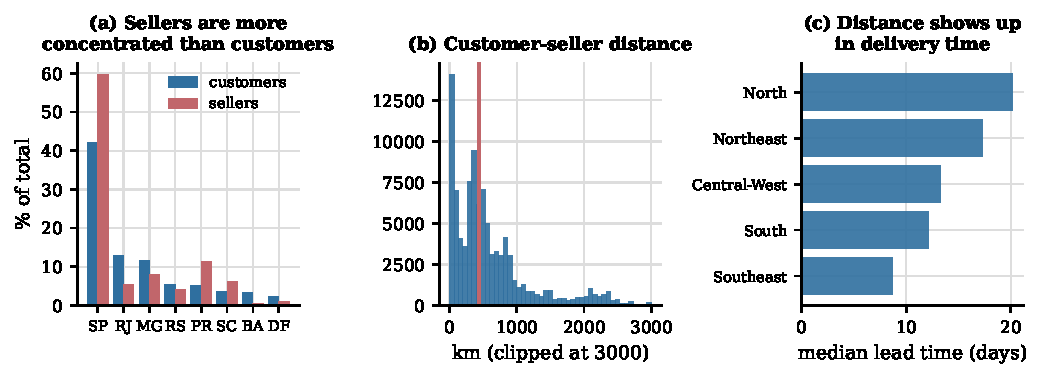
\includegraphics[width=\linewidth]{fig04_geography.pdf}
  \caption{(a) Sellers are far more concentrated in S\~{a}o Paulo than customers
  are, so most orders must cross the country. (b) Customer--seller distance.
  (c) That distance shows up directly in regional delivery times.}
  \label{fig:geography}
\end{figure}

\begin{figure}[htbp]
  \centering
  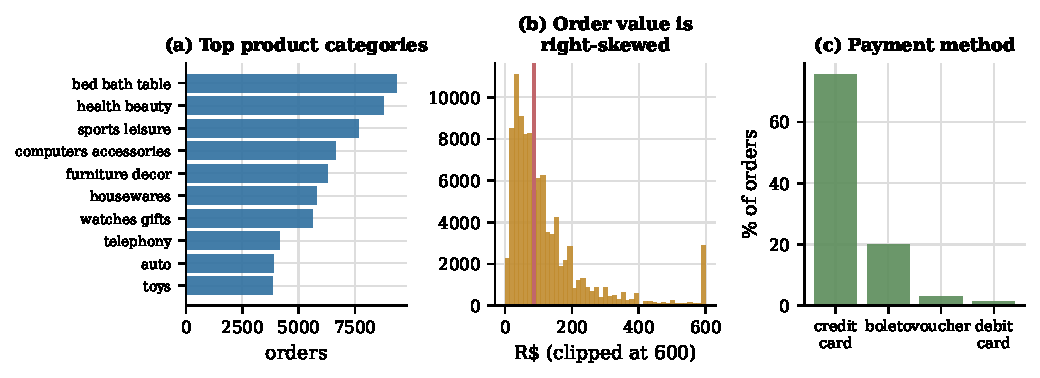
\includegraphics[width=\linewidth]{fig05_products_money.pdf}
  \caption{(a) Demand is long-tailed across 74 categories. (b) Order value is
  strongly right-skewed. (c) Credit card dominates, usually in instalments.}
  \label{fig:products}
\end{figure}

\begin{figure}[htbp]
  \centering
  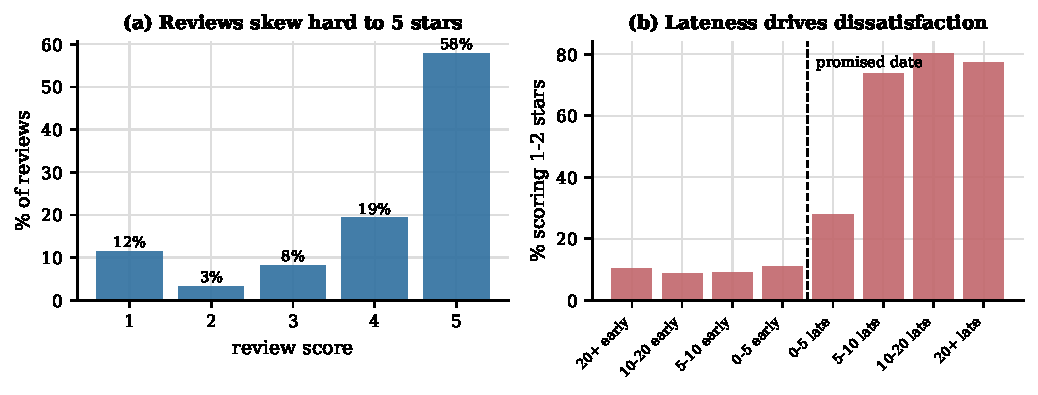
\includegraphics[width=\linewidth]{fig06_reviews_delivery.pdf}
  \caption{(a) Reviews are severely imbalanced towards five stars. (b) The
  strongest relationship in the dataset: the 1--2 star rate rises monotonically
  with lateness, from 9.2\% for on-time orders to 54.0\% for late ones.}
  \label{fig:reviews}
\end{figure}

\begin{figure}[htbp]
  \centering
  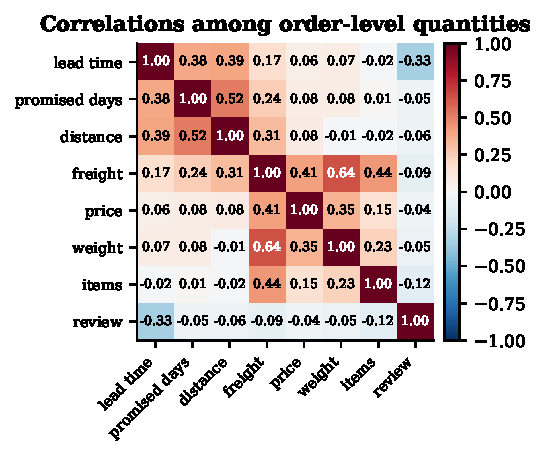
\includegraphics[width=0.62\linewidth]{fig07_correlations.pdf}
  \caption{Correlations among order-level quantities. Distance and the platform's
  own promise are the strongest checkout-time correlates of lead time; the
  review score moves with lead time and not with price.}
  \label{fig:correlations}
\end{figure}

\begin{figure}[htbp]
  \centering
  \includegraphics[width=0.58\linewidth]{fig08_leakage.pdf}
  \caption{What one forbidden column is worth. Adding the realised delivery time
  to the late-delivery model takes ROC-AUC from 0.589 to 1.000 --- the model is
  reading the answer, not predicting it.}
  \label{fig:leakage}
\end{figure}

\begin{figure}[htbp]
  \centering
  \includegraphics[width=\linewidth]{fig09_candidates.pdf}
  \caption{Candidate comparison from the scoping phase. (a) PR-AUC against the
  no-skill floor for each candidate and prediction moment. (b) Lead-time MAE:
  the platform's own promise is worse than a constant. (c) Raw accuracy flatters
  every imbalanced target; balanced accuracy does not.}
  \label{fig:candidates}
\end{figure}

\begin{figure}[htbp]
  \centering
  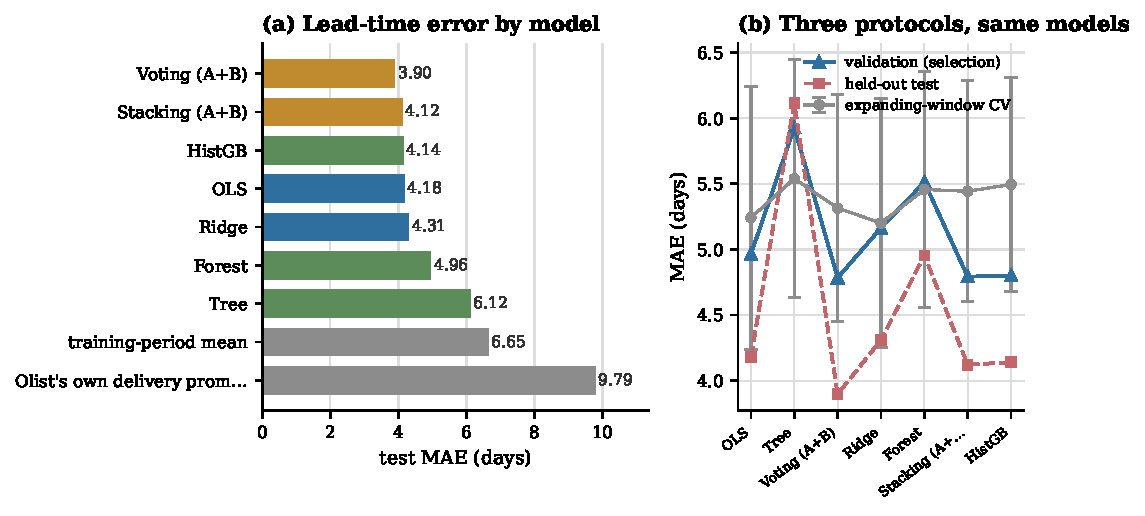
\includegraphics[width=\linewidth]{fig10_regression_ladder.pdf}
  \caption{Lead-time error by model, and the same models under three protocols.
  Panel (b) is the argument of Section~\ref{sec:cv}: expanding-window
  cross-validation does not order the candidates the way the validation period
  and the forward window --- which agree with each other --- do.}
  \label{fig:ladder}
\end{figure}

\begin{figure}[htbp]
  \centering
  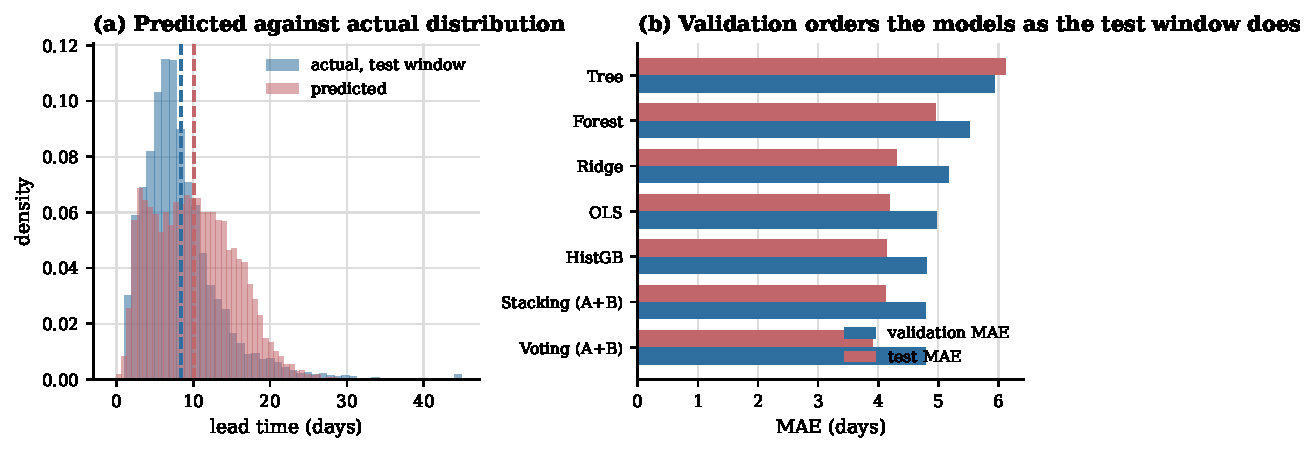
\includegraphics[width=\linewidth]{fig19_extrapolation.pdf}
  \caption{Why blending a linear model with a boosted one helps under drift. A
  tree cannot predict outside the range of the targets it was fitted on; lead
  times in the test window are systematically shorter than anything common in
  training. Panel (b) shows the validation period ordering the models as the test
  window does.}
  \label{fig:extrap}
\end{figure}

\begin{figure}[htbp]
  \centering
  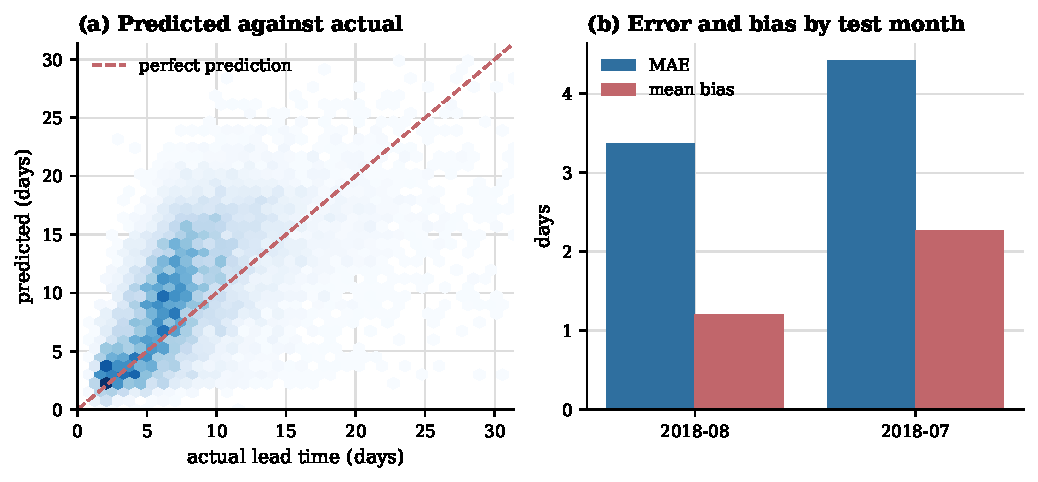
\includegraphics[width=\linewidth]{fig11_regression_residuals.pdf}
  \caption{Where the regression is wrong. The bias in panel (b) is positive in
  both test months: a model fitted on a slower past over-predicts how long a
  parcel will take.}
  \label{fig:resid}
\end{figure}

\begin{figure}[htbp]
  \centering
  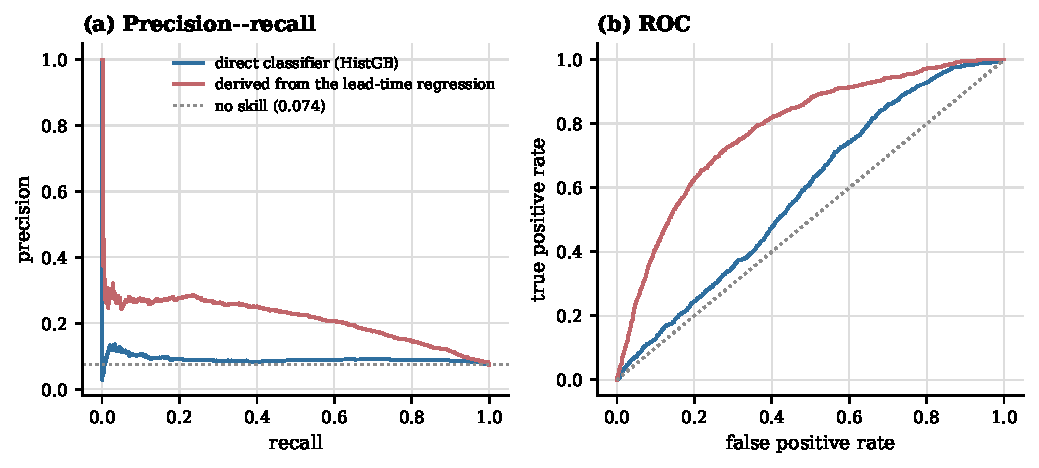
\includegraphics[width=\linewidth]{fig12_late_routes.pdf}
  \caption{Problem 1B. The flag derived from the lead-time regression against the
  best purpose-built classifier, on the forward test window.}
  \label{fig:routes}
\end{figure}

\begin{figure}[htbp]
  \centering
  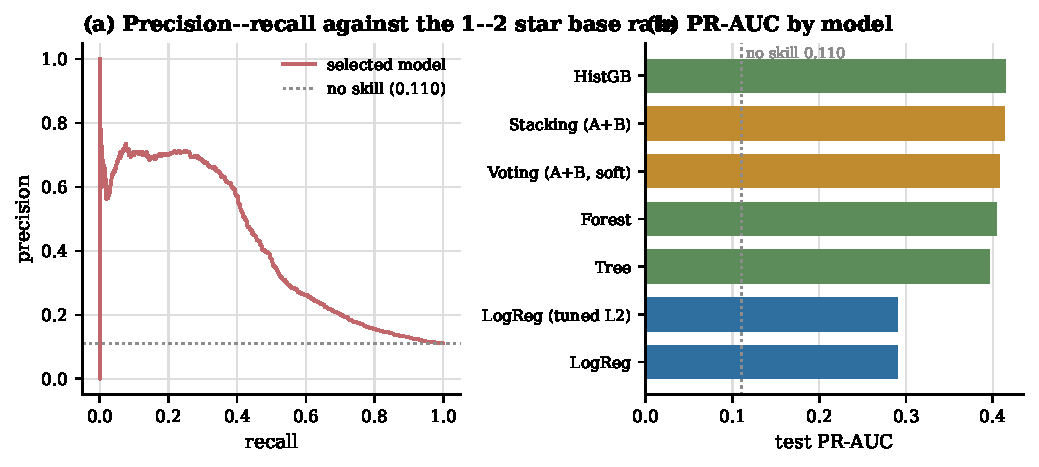
\includegraphics[width=\linewidth]{fig13_low_review.pdf}
  \caption{Problem 2 against its no-skill floor, and PR-AUC by model. Most of the
  achievable signal is already available from a single depth-limited tree.}
  \label{fig:lowreview}
\end{figure}

\begin{figure}[htbp]
  \centering
  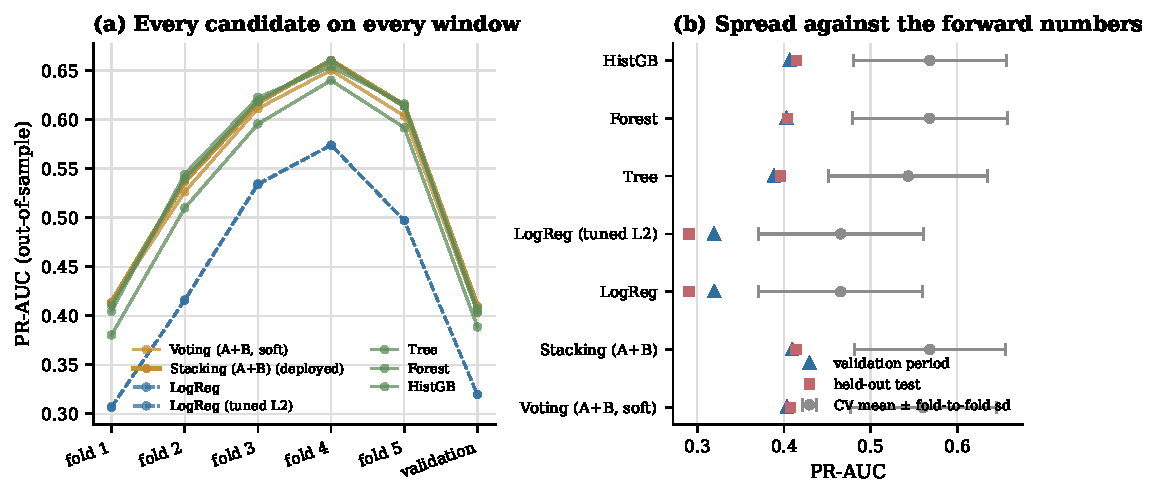
\includegraphics[width=\linewidth]{fig22_cv_folds.pdf}
  \caption{Fold-to-fold variation of every Problem 2 candidate
  (Table~\ref{tab:cvfolds}). (a) Each candidate's PR-AUC on the five expanding
  folds and the validation period: the windows move together, because their
  difficulty differs far more than the candidates do. (b) The cross-validated
  mean with its fold-to-fold standard deviation beside the validation and test
  scores: the spread is about 0.09 against a gap of under 0.001 between the best
  candidates.}
  \label{fig:cvfolds}
\end{figure}

\begin{figure}[htbp]
  \centering
  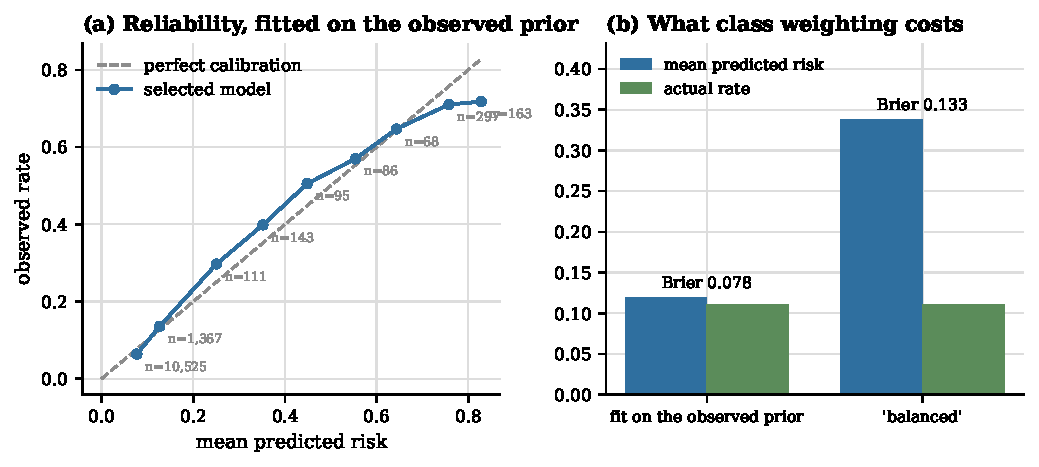
\includegraphics[width=\linewidth]{fig14_calibration.pdf}
  \caption{Calibration, and what class weighting costs. Weighting the loss leaves
  ranking unchanged and inflates mean predicted risk threefold against the actual
  rate.}
  \label{fig:calibration}
\end{figure}

\begin{figure}[htbp]
  \centering
  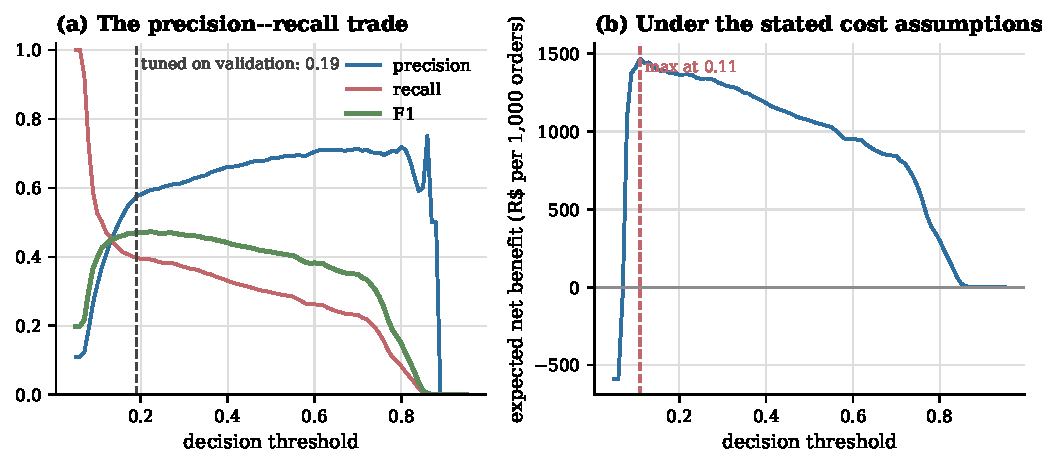
\includegraphics[width=\linewidth]{fig15_threshold_cost.pdf}
  \caption{Choosing the operating point for the review model, and what it is
  worth under the stated cost assumptions.}
  \label{fig:threshold}
\end{figure}

\begin{figure}[htbp]
  \centering
  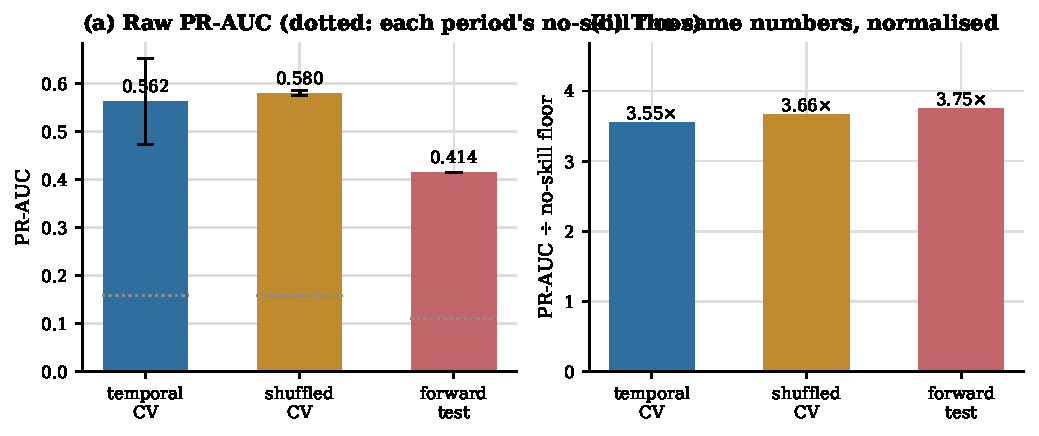
\includegraphics[width=\linewidth]{fig16_cv_protocol.pdf}
  \caption{One model, three protocols. Raw average precision disagrees across
  periods; divided by each period's no-skill floor the three agree to within 0.2
  of a multiple.}
  \label{fig:protocol}
\end{figure}

\begin{figure}[htbp]
  \centering
  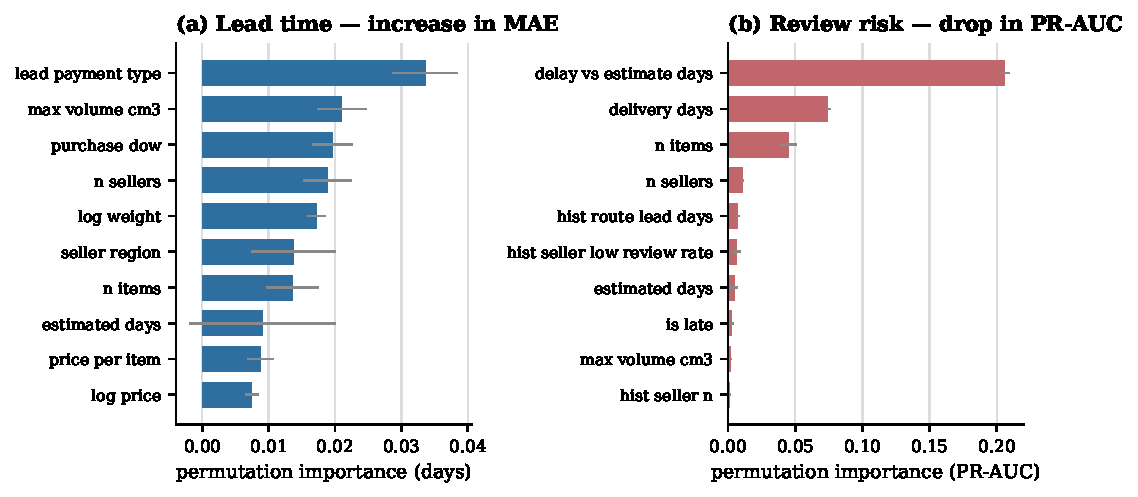
\includegraphics[width=\linewidth]{fig17_importance.pdf}
  \caption{Permutation importance on the test window. The review model rests on
  two features; the lead-time model on none in particular, which is a property of
  correlated predictors as much as of the model.}
  \label{fig:importance}
\end{figure}

\begin{figure}[htbp]
  \centering
  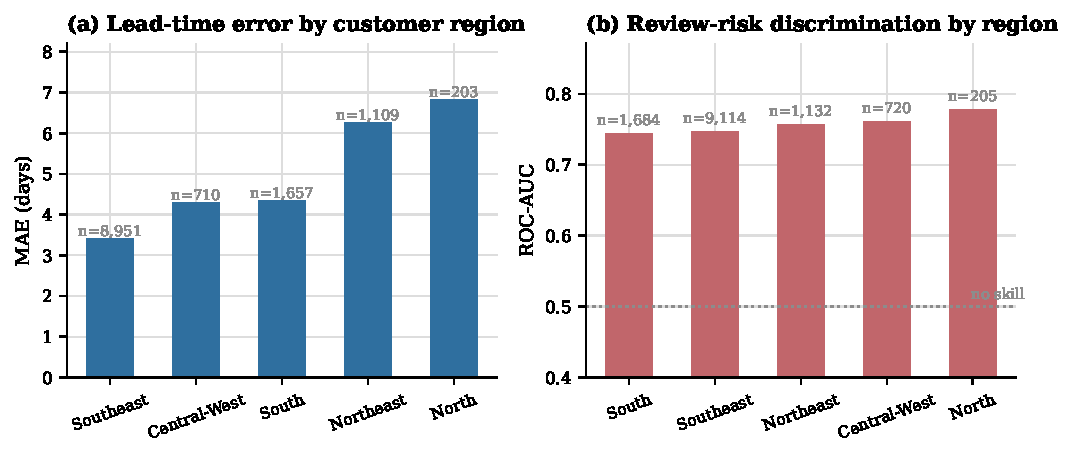
\includegraphics[width=\linewidth]{fig18_segments.pdf}
  \caption{Performance by customer region. The review model is stable across all
  five; the regression is not, and degrades exactly where deliveries are
  longest.}
  \label{fig:segments}
\end{figure}

\begin{figure}[htbp]
  \centering
  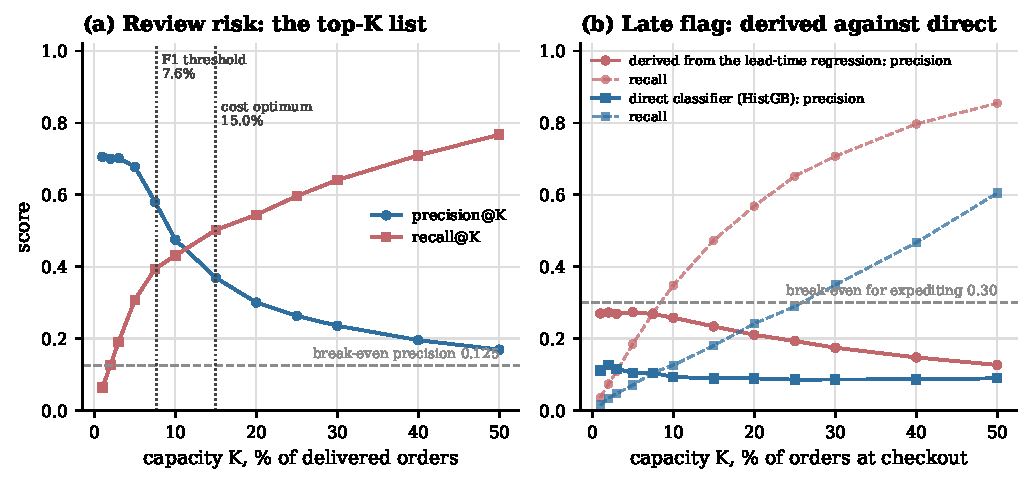
\includegraphics[width=\linewidth]{fig20_capacity.pdf}
  \caption{Precision and recall when only the top $K$ can be acted on
  (Section~\ref{sec:results-capacity}). (a) The review-risk list, with the
  report's two threshold operating points placed on the capacity axis; precision
  stays above the break-even at every capacity. (b) The late flag: the derived
  route beats the direct classifier at every $K$ and never reaches the
  break-even an expensive expedite would need.}
  \label{fig:capacity}
\end{figure}

\begin{figure}[htbp]
  \centering
  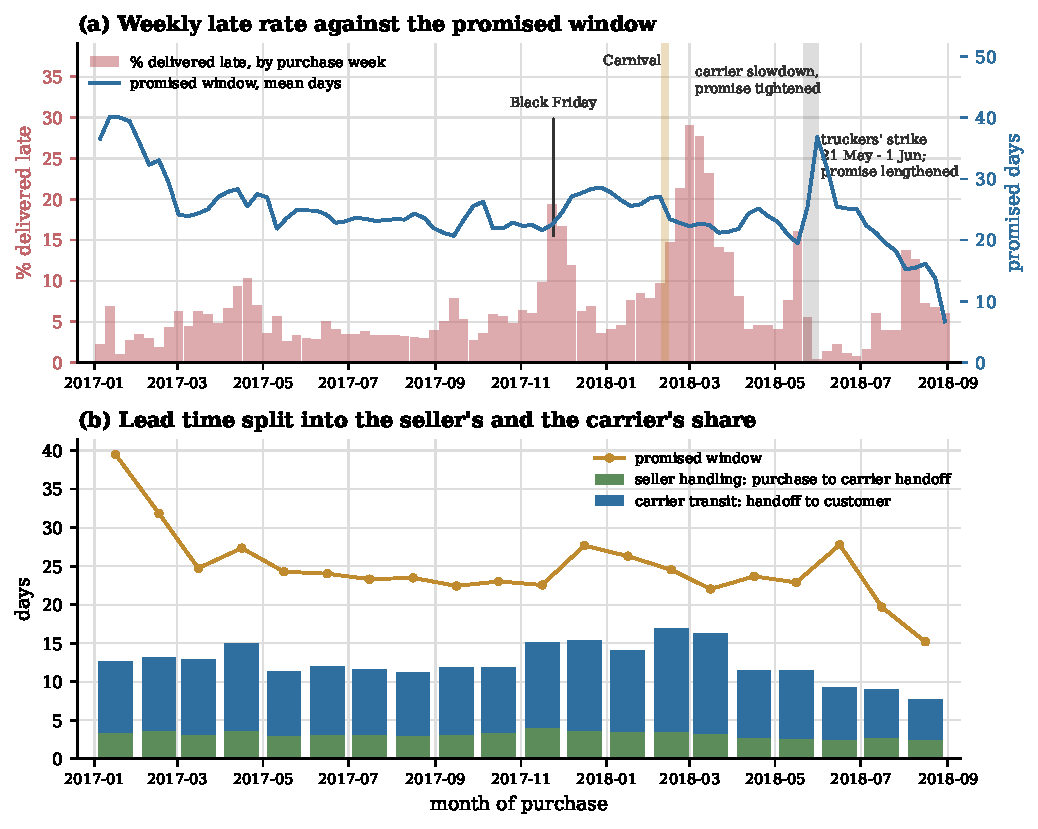
\includegraphics[width=\linewidth]{fig21_lateness_anatomy.pdf}
  \caption{Where the late deliveries came from (Appendix~\ref{app:lateness}).
  (a) Weekly late rate against the promised window: the February--March 2018
  peak coincides with a tightened promise, and the strike of 21 May--1 June 2018
  (shaded) hits the week promised before it, after which the promise is
  lengthened and the late rate collapses. (b) Lead time split at the carrier
  handoff: the peak is carrier transit, not seller handling.}
  \label{fig:lateness}
\end{figure}

\begin{figure}[htbp]
  \centering
  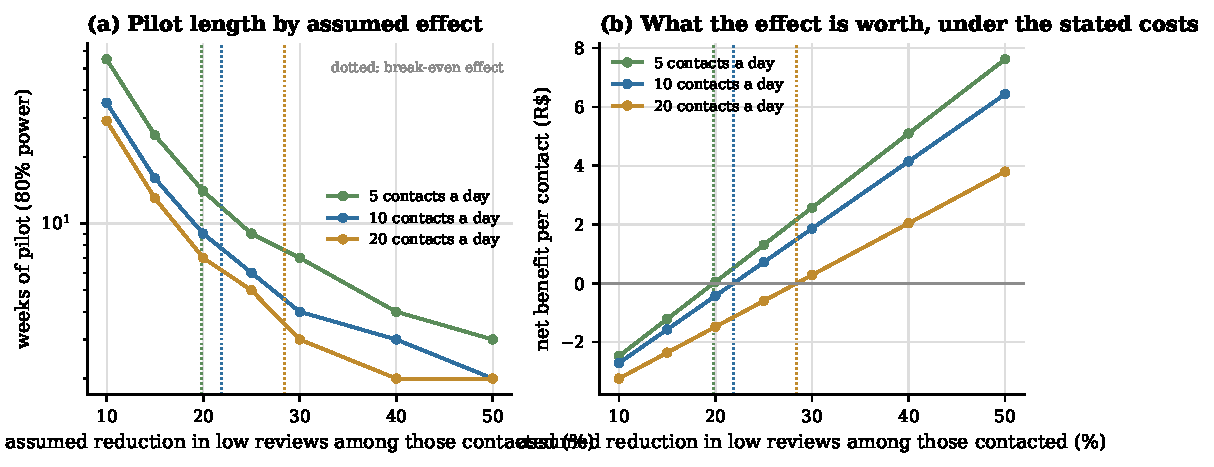
\includegraphics[width=\linewidth]{fig23_pilot.pdf}
  \caption{Sizing the outreach pilot (Section~\ref{sec:pilot}). (a) Weeks
  needed, at 80\% power, to detect a given reduction in low reviews among the
  customers contacted, for three daily capacities; the dotted lines mark each
  capacity's break-even effect. (b) The net benefit per contact that reduction
  would imply under the stated costs.}
  \label{fig:pilot}
\end{figure}

\begin{figure}[htbp]
  \centering
  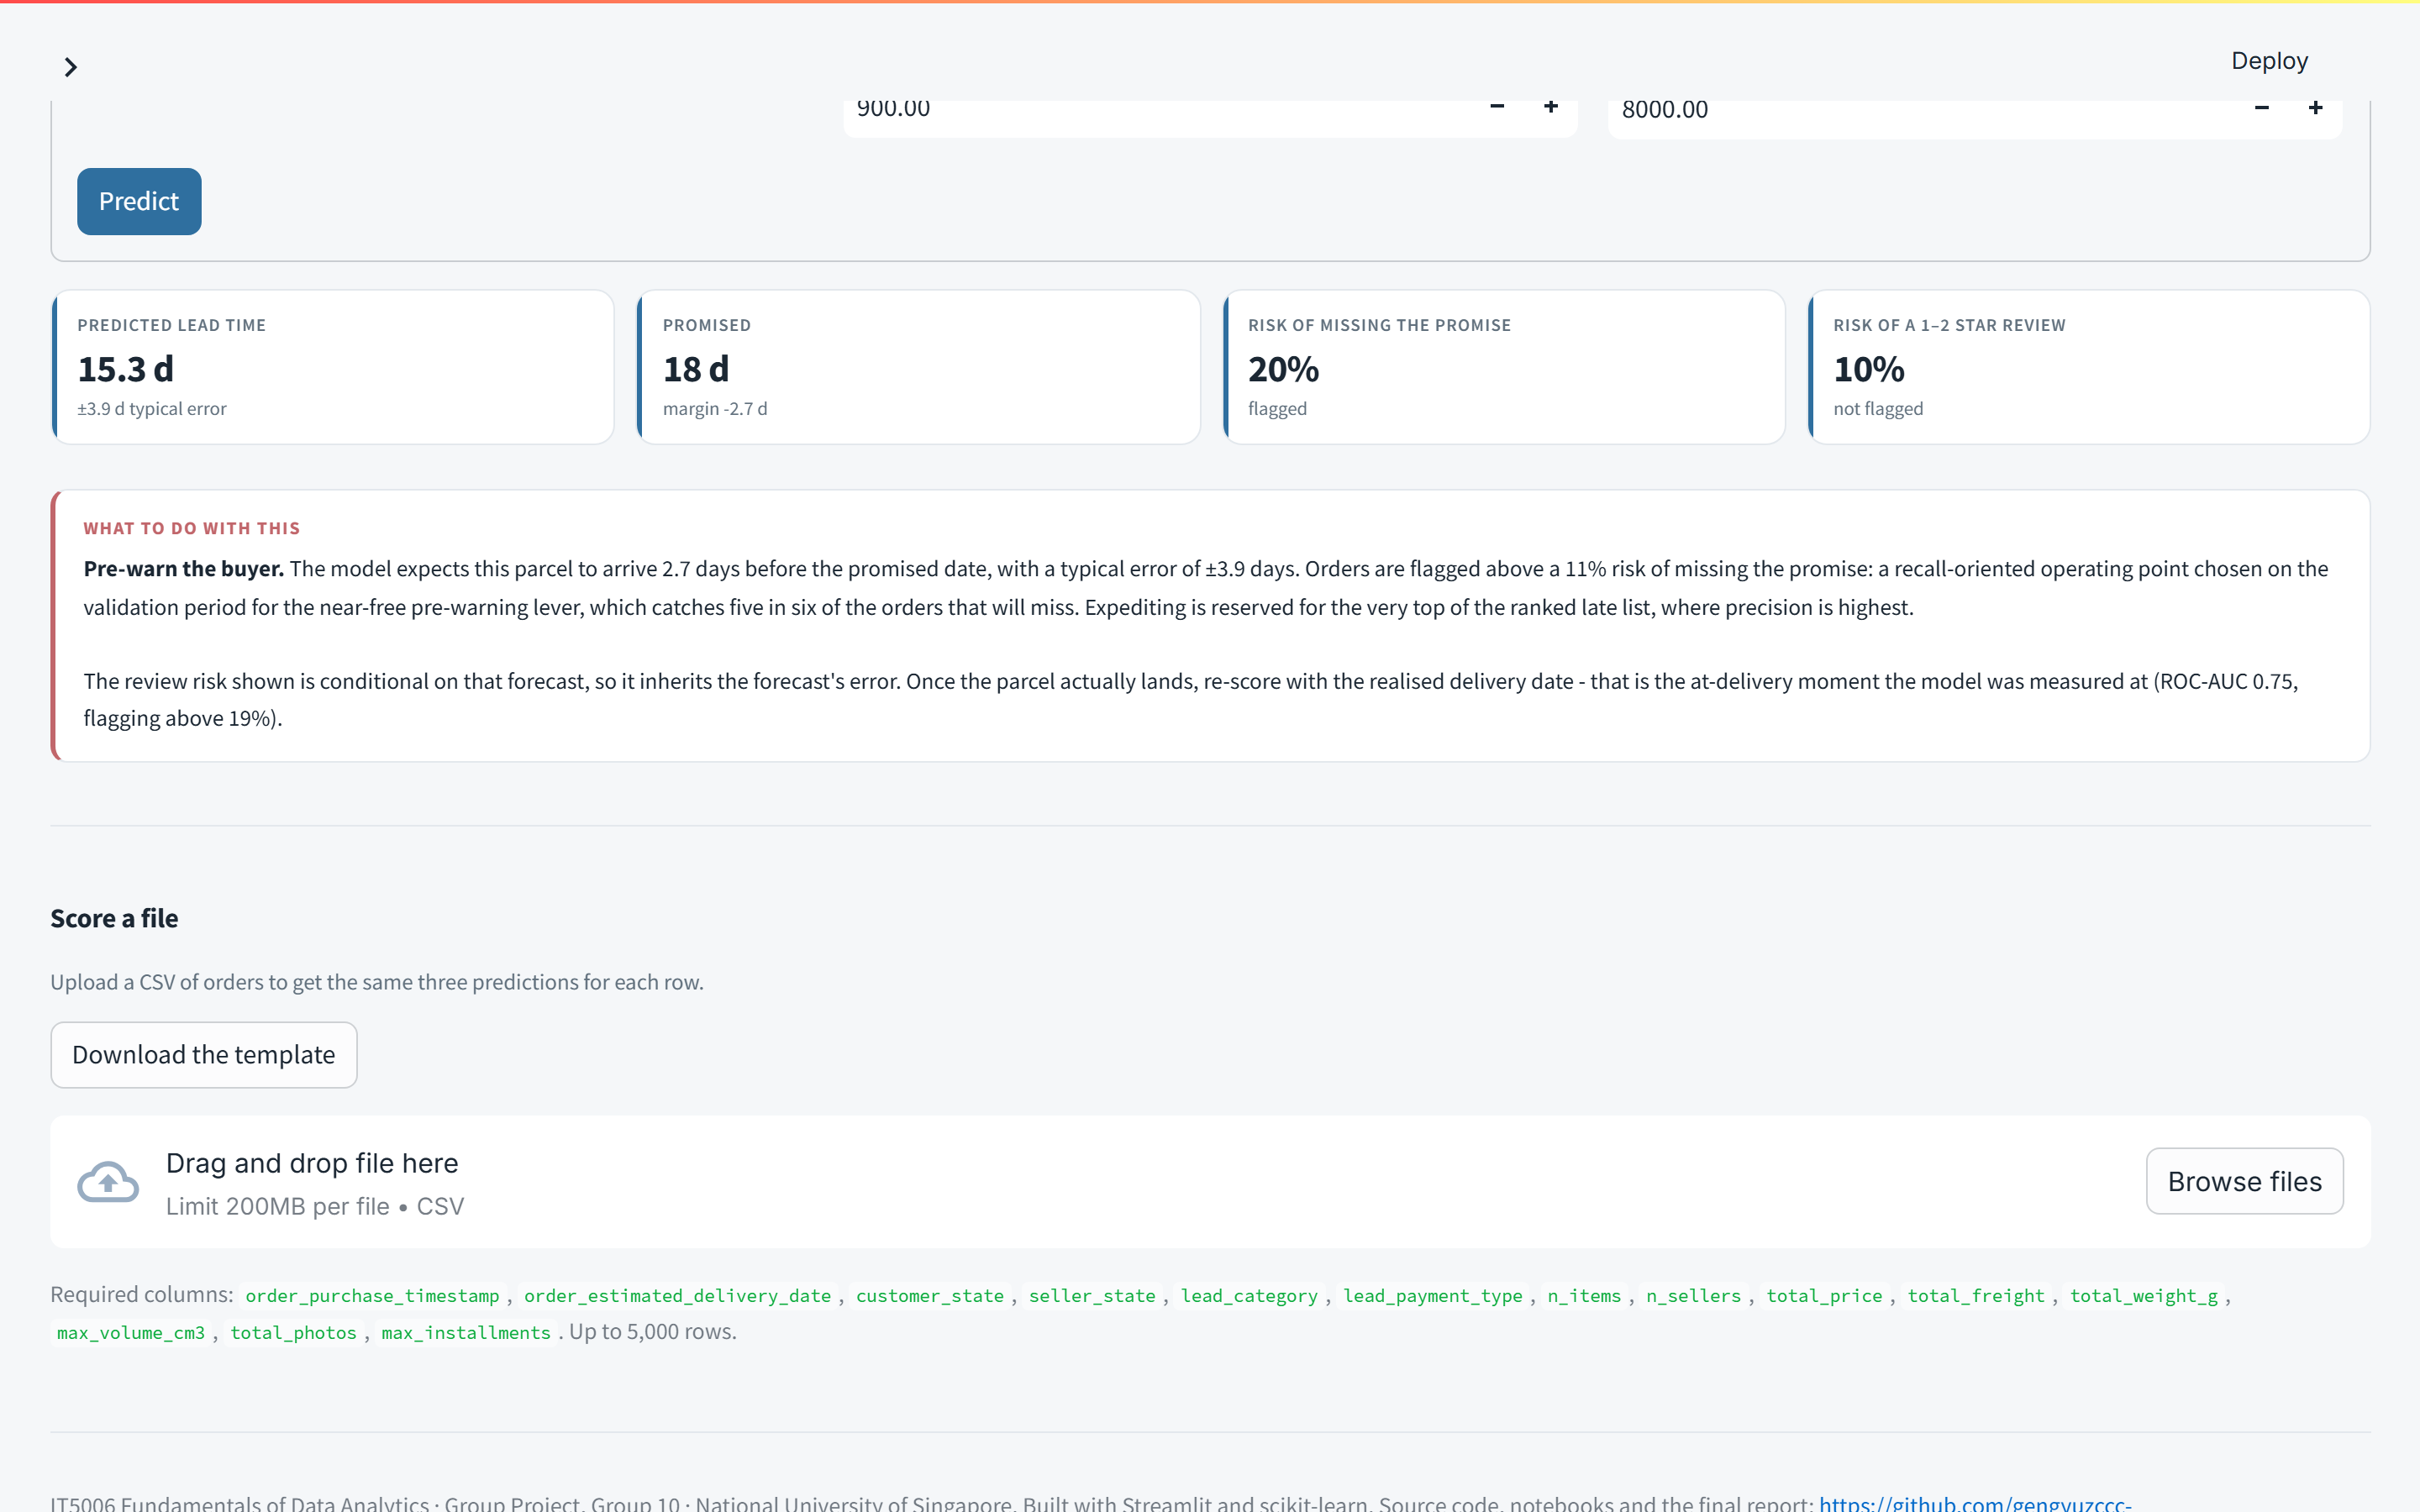
\includegraphics[width=\linewidth]{app_predict.png}
  \caption{The deployed application, Predict tab: one order scored at checkout
  --- expected lead time, the risk of missing the promise against the tuned
  threshold, and the resulting review risk --- with the batch scorer and the
  top-$K$ triage list below.}
  \label{fig:app-predict}
\end{figure}

\begin{figure}[htbp]
  \centering
  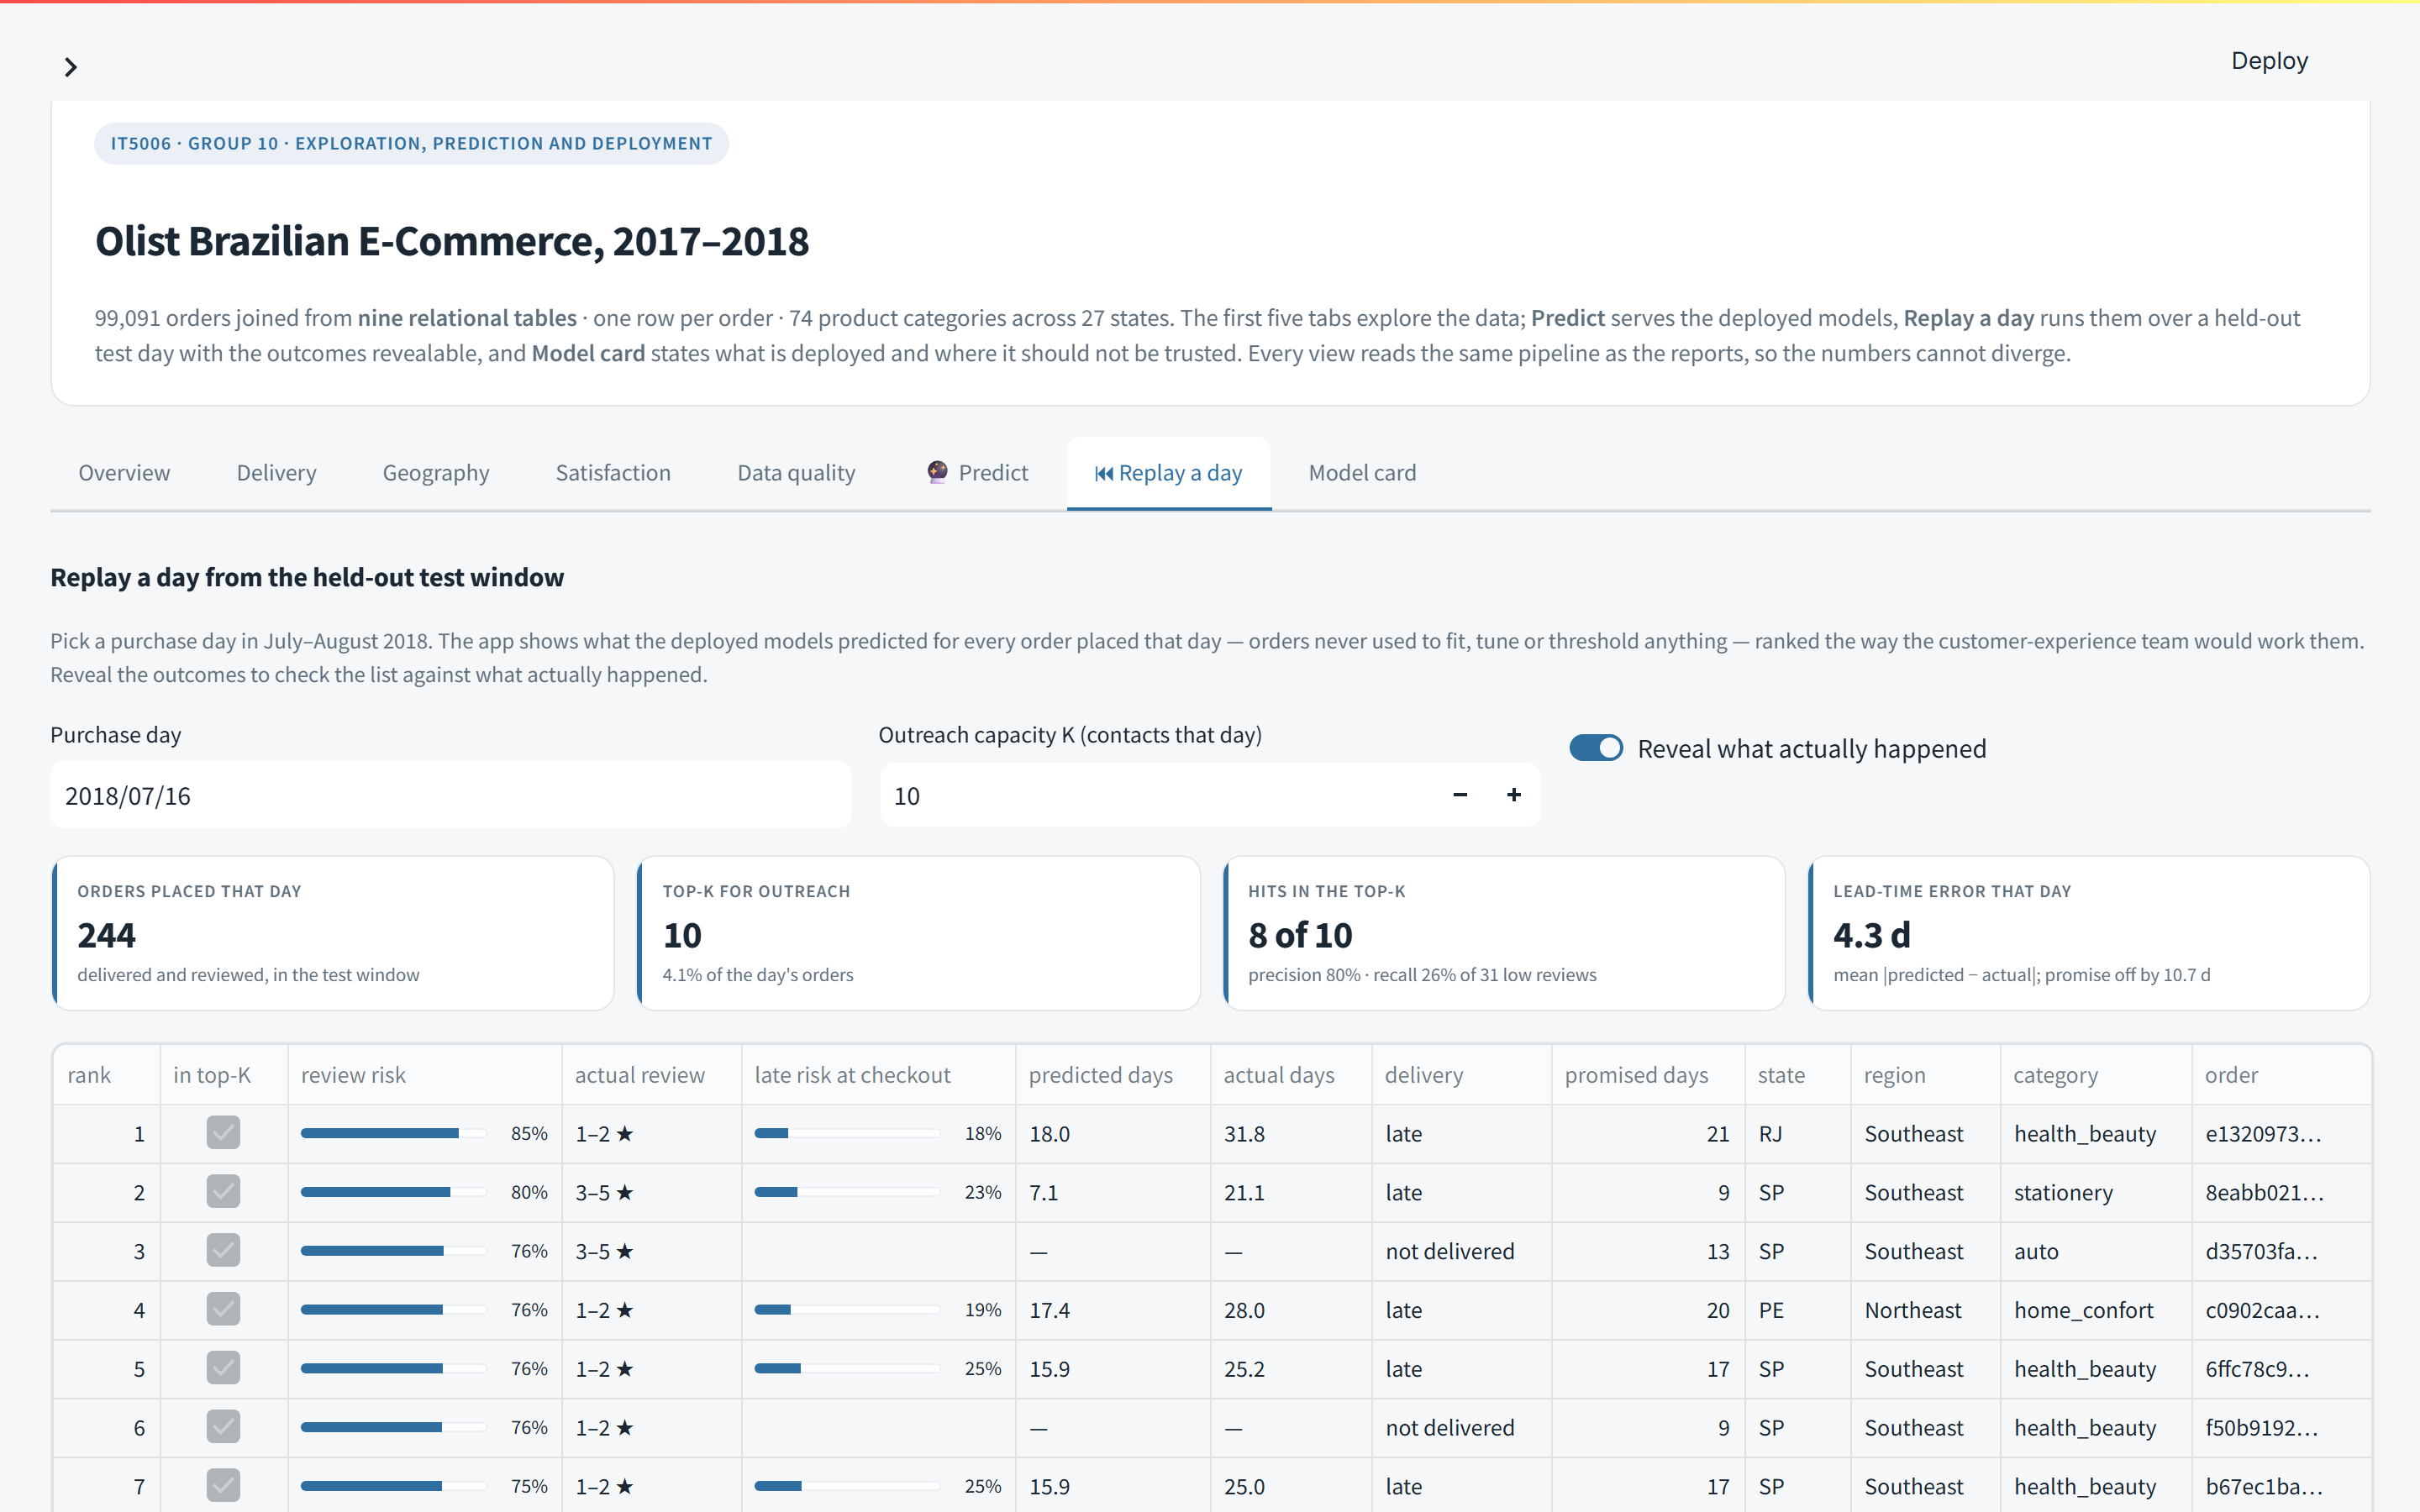
\includegraphics[width=\linewidth]{app_replay.png}
  \caption{The deployed application, Replay a day: the held-out orders placed on
  16 July 2018 ranked by review risk with a capacity of ten, outcomes revealed.
  Eight of the ten would have reached a customer who left a 1--2 star review;
  the right-hand panel shows the same capacity's precision on every day of the
  test window.}
  \label{fig:app-replay}
\end{figure}

\begin{figure}[htbp]
  \centering
  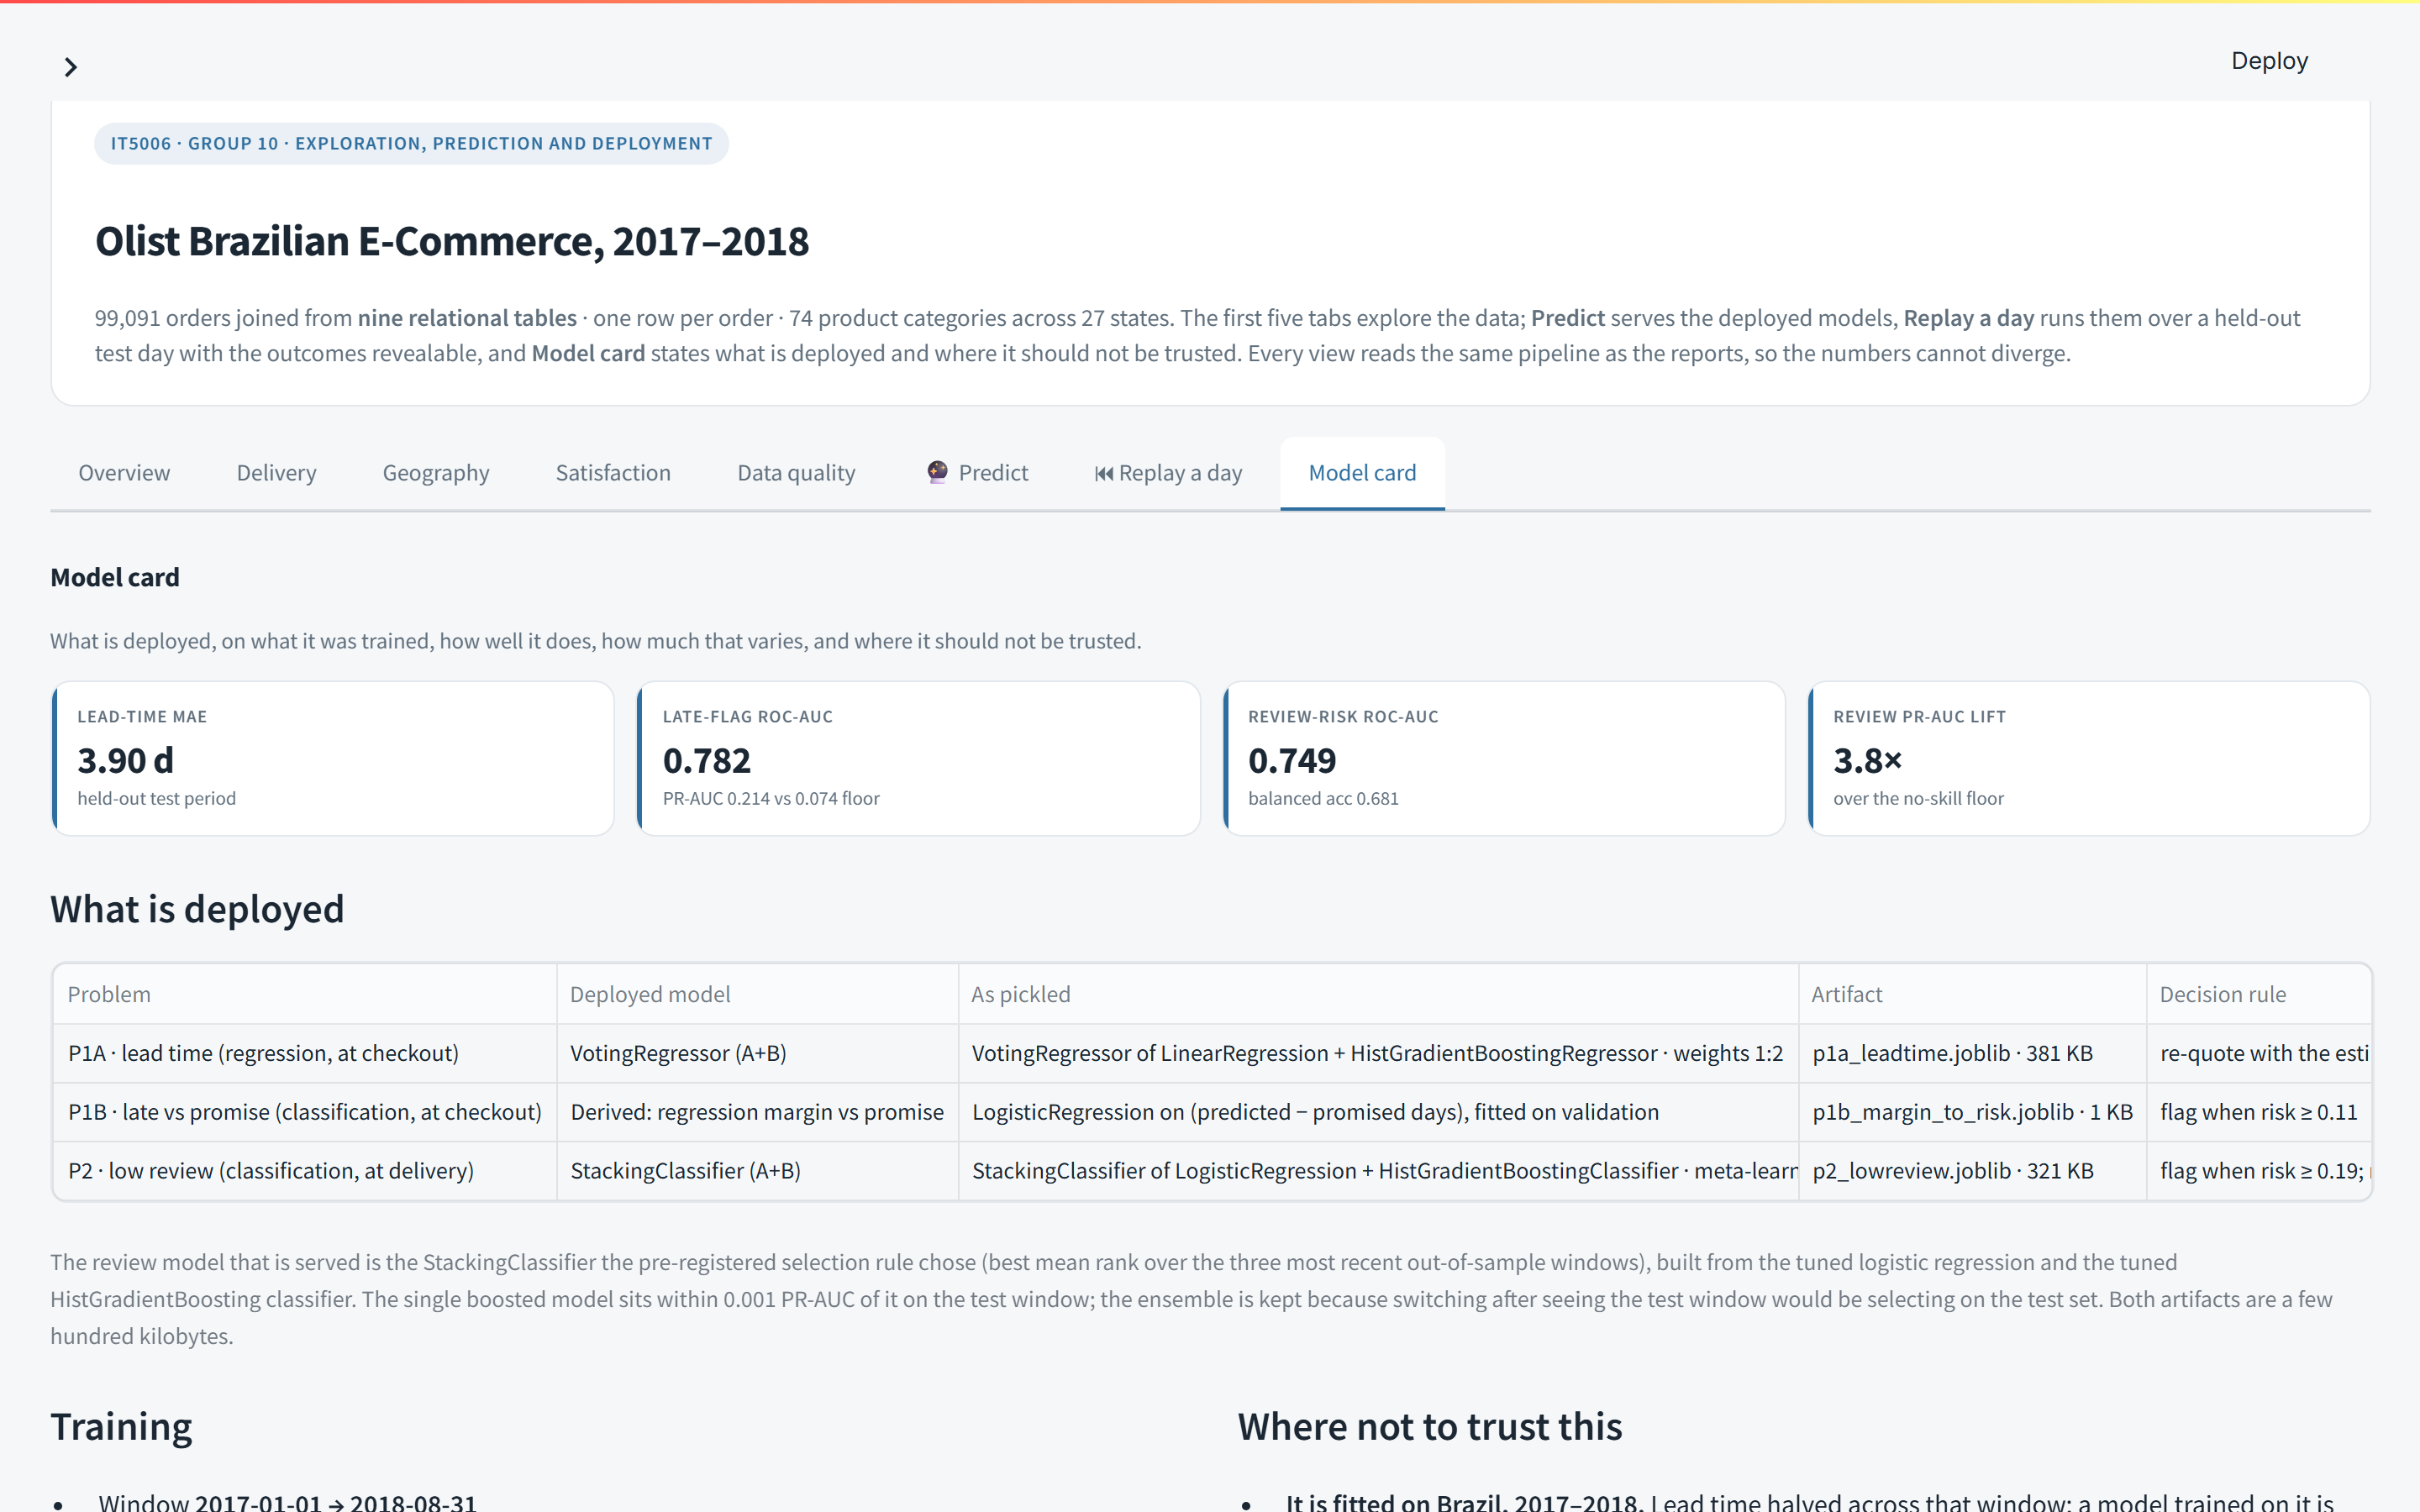
\includegraphics[width=\linewidth]{app_card.png}
  \caption{The deployed application, Model card: the estimators as pickled, the
  training protocol, where the models should not be trusted, and the
  fold-to-fold table.}
  \label{fig:app-card}
\end{figure}


% ============================== AI DECLARATION =============================
\clearpage
\section*{AI Tool Declaration}
\addcontentsline{toc}{section}{AI Tool Declaration}

We used OpenAI's ChatGPT and Anthropic's Claude to generate and validate ideas,
improve expression and refine our writing. We also used the models to debug our
code. All analytical decisions, results and conclusions were reviewed and
verified by the team against the underlying data, and we are responsible for the
content and quality of the submitted work.

\end{document}
